
\documentclass[master]{thesis-uestc}

\title{复杂推理的起点:知识库在视觉问答的应用}{The Start of Complex Reasoning: The Application of Knowledge Base in Visual Question Answering}

\author{陈小兵}{Xiaobing Chen}
\advisor{郑文锋\chinesespace 副教授}{Dr. Wenfeng Zheng}
\school{自动化工程学院}{School of Automation Engineering}
\major{控制科学与工程}{Control Science and Engineering}
\studentnumber{201721070835}

% require all the usepackages here
% \usepackage{algorithm2e}

\begin{document}

\makecover

% This is a template of mutiple files.
% The folders chapters/ and misc/ have the related files

% abstract
	
\begin{chineseabstract}
视觉问答是给定一张图片和一个图像相关的自然语言问题,输出问题答案的人工智能任务。跨领域的视觉问答接近通用人工智能,有很高的研究价值和广阔的应用场景。按照是否引入外源知识库,现有模型分为联合嵌入模型和基于知识库的模型,这两类模型在视觉问答任务中均有不错的表现。然而主流的联合嵌入模型存在数据集依赖、网络容量小和文本表征能力不足的缺陷。另一方面,通过引入外源知识库,基于知识库的模型克服了联合嵌入模型的网络容量限制,能回答涉及常识或外源知识的推理问题。但其需要通过人工构建知识库查询语句,极大的限制了模型的泛化能力。本文分别改进了联合嵌入模型的文本特征化方法和基于知识库的模型的通用性,主要包括以下内容:

1)引入动态词向量改进联合嵌入模型的文本特征化方法。目前的联合嵌入模型的文本特征化方法仍然使用静态词向量方法,考虑到静态词向量无法有效表征一词多义和一词多用的情况,本文在视觉问答模型中引入动态词向量,并结合Faster R-CNN和注意力机制,提出了基于动态词向量的联合嵌入模型(N-KBSN)。实验结果证明动态词向量能实现更好的文本特征表示,进而提高准确率。

2)构建了一个知识库图嵌入模块,以扩展基于知识库的模型的通用性。本文构建的知识库图嵌入模块分别从图像和文本中提取核心实体,并映射为知识库实体,再以核心实体为中心提取出子图,并将子图转换为低维向量,实现子图嵌入。为了实现好的子图嵌入,我们首先从DBpedia中提取了两个具有丰富语义的实验知识库:DBV和DBA。并基于这两个知识库,选取了一系列知识库嵌入模型进行链路预测实验。实验结果显示,DBV知识库的实体间具有清晰的对应关系,能实现优异的节点嵌入。并且TransE模型能实现很好的知识库嵌入,因此我们以TransE为核心构建了知识库图嵌入模块。

3)合并知识库图嵌入模块和N-KBSN模型,构建了基于知识库图嵌入的视觉问答模型(KBSN)。在多个数据集上的实验结果证明,知识库图嵌入模块提高了视觉问答的准确率。尤其在面对需要常识或外源知识的复杂问题时,准确率提升明显。

\chinesekeyword{视觉问答,联合嵌入模型,知识库,N-KBSN,KBSN}
\end{chineseabstract}



\begin{englishabstract}
Visual Question Answering (VQA) is an artificial intelligence task that outputs an answer to a question given a picture and a related natural language question. Compared with other tasks, VQA is closer to General Artificial Intelligence(GAI). Therefore, the research of VQA model has high research value and promising application scenarios. According to whether the knowledge base is introduced, the existing models are divided into joint embedding models and knowledge base-based models. These two types of models have good performance in VQA tasks. However, the mainstream joint embedding model has the defects of data set dependence, small network capacity and insufficient text representation ability. On the other hand, by introducing an external knowledge base, the knowledge base-based model overcomes the network capacity limitation of the joint embedding model and can answer inference questions involving common sense or external knowledge. However, it needs to construct knowledge base query statements manually, which greatly limits the generalization ability of the model. This paper improves the text representation method of the joint embedding model and the generality of the model based on the knowledge base, mainly including the following:

1) Introduce dynamic word embeddings to improve the text characterization method of the joint embedding model. The current text embedding method of the joint embedding model still uses the static word embedding method. Considering that the static word vector cannot effectively represent the polysemy and multi-word, our paper introduces dynamic word embeddings to the VQA model, combining Faster R-CNN and attention mechanism, proposed a joint embedding model (N-KBSN) based on dynamic word embeddings. The experimental results prove that the dynamic word embedding can achieve better text feature representation, thereby improving accuracy. The accuracy of a single N-KBSN modle on the VQA2.0 data set have exceeded the champion model of the 2019 public challenge.

2) Construct a knowledge base graph embedding module to extend the versatility of knowledge-based models. The knowledge base graph embedding module constructed in this paper extracts core entities from images and text, and maps them as knowledge base entities, then extracts the sub-graphs closely related to the core entities, and converts the sub-graphs into low-dimensional vectors to realize sub-graph embedding. In order to achieve good subgraph embedding, we first extracted two experimental knowledge bases with rich semantics from DBpedia: DBV and DBA. Based on these two knowledge bases, a series of knowledge base embedding models are selected to produce link prediction. The results show that there is a clear correspondence between the entities of the DBV, which can achieve excellent node embedding. And the TransE model can achieve a good knowledge base embedding, so we built the knowledge base graph embedding module based on TransE.

3) Merge the knowledge base graph embedding module and the N-KBSN model, and construct a VQA model (KBSN) based on the knowledge base graph embedding. Experimental results on multiple data sets prove that the knowledge base graph embedding module improves the accuracy of VQA. The accuracy improves significantly while processing complex problems that require common sense or external knowledge.
	
\englishkeyword{Visual Question Answering, Joint Embedding Model, Knowledge Base, N-KBSN,KBSN}
\end{englishabstract}




% table of contents
\thesistableofcontents

% thesis contents
\thesischapterexordium

\section{研究工作的背景与意义}

视觉问答是近几年学界新兴研究的热门方向之一。得益于神经网络架构在自然语言处理和图像识别相关任务的成功应用,学界将研究的视线移向对系统智能要求更高的视觉问答任务。视觉问答任务是一类输入为图像和用自然语言表达的文本问题,输出为基于图像内容理解并且用自然语言方式呈现的答案的计算机视觉任务。简而言之,任务目标是构建一个像人类智能一样的问答系统——能够从给定的图片中,抽象凝结出图中物体的类别、空间关系、活动、场景等高阶信息;并根据问题的不同,针对性得给出合理的答案。

视觉问答的问题类型包含二值的是否问题\citing{krishna2017visual,zhu2016visual7w,andreas2015deep}、多选问题\citing{antol2015vqa,zhu2016visual7w}、开放性问题\citing{antol2015vqa},涉及诸多计算机视觉中的子任务\citing{kafle2017visual},例如:
\begin{description}[labelindent=2em, leftmargin=6em, style=sameline]
\item [物体识别]——图片中有哪些动物?
\item [物体检测]——图片中是否有小狗?
\item [属性分类]——图片中小狗的眼睛是什么颜色?
\item [场景分类]——图片中的小狗在什么地方?
\item [计数问题]——图片中有几只小狗?
\end{description}
除了以上列出的集中问题类型以外,在真实的人类交流中,更多的是具有更深层次、更复杂的问题。例如:“图片中有什么东西在伞下?”——需要能准确识别物体的空间位置关系、“图片中的交通路口是否可以通行?”——需要基于常识的推理、“图片中的汽车属于什么品牌?”——需要基于外部专业知识库提供隐藏信息。

对问题中涉及的计算机视觉任务细分,我们可以将视觉问答分为识别和推理两大任务范畴。就识别任务而言,包括物体识别、物体检测、属性分类、计数问题、空间关系判定,此类任务在以往的计算机视觉的研究中已经达到了较高的识别准确率,在某些物体识别和物体检测任务上已经能迫近甚至超越人类水平,虽然识别任务中仍然有许多值得研究的部分,但从研究的结构和难度上来看,只能算是相对简单的“点问题”。与之对应的便是更为复杂的”逻辑推演问题“,包括场景分类、知识库推理,常识推理可以被视为一种“隐知识库推理”。识别任务是逻辑推演的“前奏”,准确的识别将构成逻辑推演的“节点”,而逻辑链条中节点之间的“有向线段”则代表推理的过程(如图\ref{logic}),推理过程的构建才是推理任务的复杂之处,也是视觉问答任务的“最璀璨的明珠”。
\begin{figure}[H]
	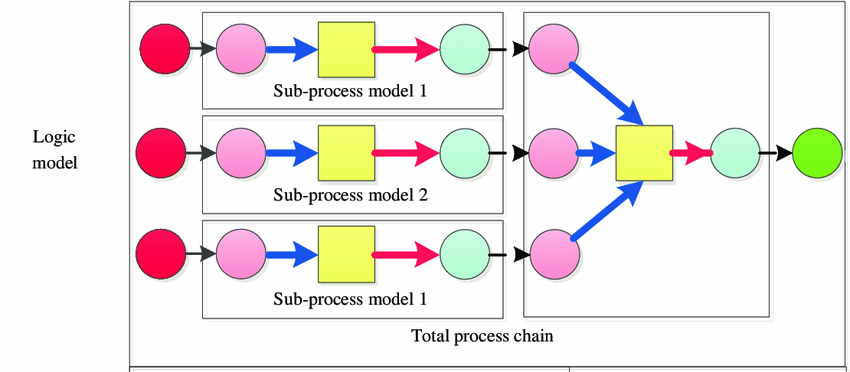
\includegraphics[width=0.8\textwidth]{logic.png}
	\caption{逻辑链中的“节点”是文本或图像上的关键信息,例如物体名称、类别、属性、关系等,“有向线段”表示“节点”间的逻辑关系}
	\label{logic}
\end{figure}

视觉问答主要涉及计算机视觉、自然语言处理、知识表达与推理三个领域。作为一个多学科交叉的领域,想实现高准确率的系统表现,既依托单个分支下理论、算法、应用系统的快速发展,作为其基础设施;同时还对各算法、子系统结合时的性能融合、体系结构提出了更多、更新的研究要求。这既是多学科高度融合状况下的挑战,也是令人兴奋不已的。正是由于视觉问答任务需要处理语言和图像两种重要的数据类型,这使得智能体更像人类一般思考和推理。智能体的“视觉系统”能够接收含有深层次信息的图像源;智能体的“神经系统”能解析图像信息和理解语言内涵;智能体的“语言系统”能够遣词造句,输出人类可理解的语言形式。因此视觉问答被认为是人类构建“人工智能完全体”的重要一步\citing{ antol2015vqa, malinowski2014towards, geman2015visual}。

视觉图灵测试\citing{geman2015visual}是一种能够衡量智能体系是否在图像语义理解方面达到人类水平的测试方法,视觉问答任务被认为是智能系统通过视觉图灵测试的关键性技术。除了作为图像理解的图灵测试的核心部分,视觉问答还有其他具有价值的应用场景。a)作为盲人或是有视觉障碍问题的病患的辅助系统,他们可以通过自然语言询问,就能获得细粒度的图像或者视频信息,能极大地帮助其获得场景的语义理解,在互联网和现实场景中均能作为一种便利的“视觉补充”。b)作为一种扩充人机交互的方式,在人机交互上可以实现多种的便利查询。通过对已有图像的询问,获得更深层次的背景知识,例如,对一副未曾见过的艺术名画询问其作者和作画背景,可以更深入的理解图像背后隐藏的人文和历史知识。通过源图像可以搜索具有相似“特征”的图像,例如,向系统查询一张埃菲尔铁塔的夜景图,将能获得更多具有相关特征的图像素材。同样可以通过图像描述查询到对应或者相似的图像。

总的来说,作为一个跨领域的人工智能任务,视觉问答代表着研究者对未来“通用人工智能”的探索,既能够提供一种跨模态的数据处理方式,又能够向机器理解和解决复杂问题,甚至完成推理的人工智能新阶段迈进。


\section{视觉问答的国内外研究状况}
视觉问答任务广阔的应用场景和对人工智能发展的深远意义驱动着研究者不断细化、泛化视觉问答的问题深度、数据集构建、算法演化。



视觉问答任务要求系统能同时正确理解问题文本内容和图像内容,一般而言视觉问答系统分为三个主要模块,a)从问题文本中提取特征,使得特征中包含足够多的语义信息。b)从图像中提取特征,理解图像中的物体信息、场景信息、活动信息、空间构成信息、颜色信息,将像素信息转化为系统可计算的数值量或者标签。 c)采用某种方式整合文本特征和图像特征,为系统建立一条高泛化能力、高稳健性、高准确率的答案生成通路。简而言之,视觉问答系统会图形和问题文本中分别提取特征,再将两者融合,最终以置信度高的候选答案作为输出(如图\ref{answer-generation})。

从视觉问答的处理过程可以看出,算法的核心有三个部分组成:如何提取出高层次的图像特征,例如,物体、属性、场景等;如何挖掘问题文本中的语义信息,以求能深入的理解问题内容,确定答案的形式和内容;如何结合图像特征和文本特征,得出正确或是最佳答案。受神经网络在计算机视觉和自然语言处理成功应用的影响,从2014至今的视觉问答研究多采用了神经网络模型,使用卷积神经网络CNN提取图像特征,使用卷积神经网络RNN或者长短期记忆LSTM处理文本信息,再通过不同的方式“融合”图像特征和文本特征得出答案。图像特征提取的方法一般使用预处理后的卷积神经网络,例如VGGNet\citing{simonyan2014very}、 ResNet\citing{he2016deep}和GoogLeNet\citing{Szegedy_2015_CVPR}。问题文本的特征提取则借鉴了自然语言处理中的成果,例如词袋模型(BOW)\citing{zhou2015simple}、长短期记忆(LSTM)\citing{malinowski2015ask}、门控复发单位(GRU)\citing{noh2016image,kumar2016ask,xiong2016dynamic}。系统输出答案的方式有两种(如图\ref{answer-generation}),最常见的方式是将任务视为分类问题,根据候选项的概率大小,确定答案。第二种方式则直接由系统遣词造句合成答案语句,此类方法多出现在有额外知识库的视觉问答系统中,例如Attributes-LSTM\citing{wu2016value}、ACK\citing{wu2016ask}、Ahab\citing{wang2015explicit}、Facts-VQA\citing{wang2017fvqa}、Multimodal KB\citing{zhu2015building}。
\begin{figure}[H]
	\centering
	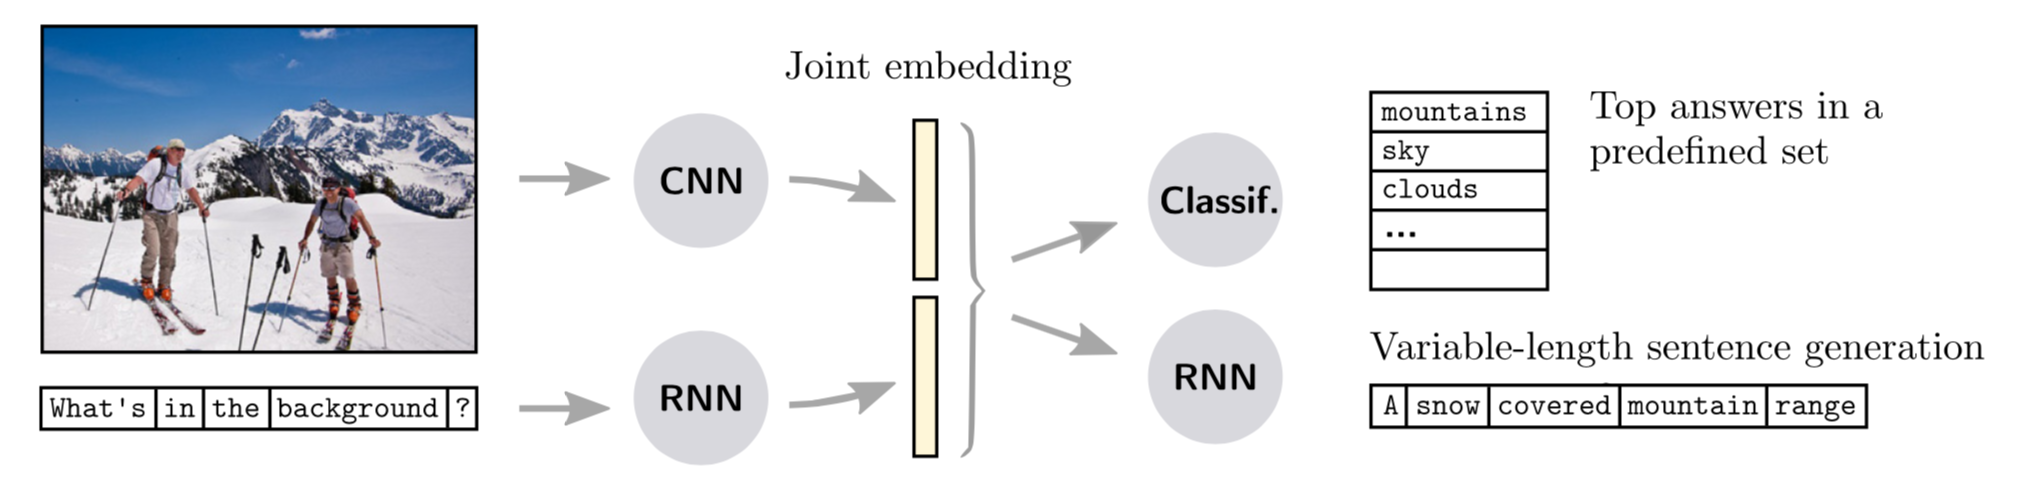
\includegraphics[width=0.8\textwidth]{answer-generation.png}
	\caption{常见的VQA方法是将图像和问题文本映射到同一特征空间,再组合融合两者的形成新的特征向量,特征向量作为分类器或者循环神经网络RNN(也可能是长短期记忆LSTM)的输入,输出得到最终的答案}
	\label{answer-generation}
\end{figure}

本节将简要介绍视觉问答方法中的联合嵌入模型、注意力机制以及动态记忆网络以及基于知识库的视觉问答方法。

\subsection{联合嵌入模型}
联合嵌入模型先将视觉信息和问题文本信息分别特征化,再通过特征向量串联\citing{zhou2015simple}、卷积\citing{ma2016learning}、逐元素相乘\citing{antol2015vqa}、逐元素相加\citing{malinowski2015ask}等池化方法融合图像特征和文本特征,最终得到最优答案。自从深度神经网络在计算机视觉和自然语言处理上的广泛应用以来,将各种模态的信息映射成特征向量的思想便大行其道,因此作为交叉领域中的视觉问答任务自然将多模信息联合嵌入到特征空间视为最“本能”的探索路径。

Malinowski等人首次提出了应用于真实场景视觉问答任务的联合嵌入模型Neural-Image-QA
\citing{malinowski2015ask}。Neural-Image-QA是一个由卷积神经网络CNN和长短期记忆LSTM组成的深度网络,先使用在ImageNet预处理过的卷积神经网络CNN对图像进行特征提取,得到的特征向量和问题文本一起传输到长短期记忆LSTM中,从而生成答案的单词序列。模型在DAQUAR数据集上完成训练和测试,对于答案只有一个词语的问题,准确率为19.43\%,对于答案是多个词语的问题,准确率为17.49\%。

Gao等人提出了mQA模型用于解决视觉问答任务\citing{NIPS2015_5641},mQA由四个部分构成,用于提取问题特征的长短期记忆LSTM(Q)、用于提取视觉特征的卷积神经网络CNN、用于存储具有多词的答案的语义上文的长短期记忆LSTM(A)、用于融合问题特征和已有的部分答案的语义特征并且预测答案的下一个词语的部分。提取视觉特征的CNN采用在ImageNet分类任务上预处理的卷积神经网络,在训练过程中保持不变,训练其他三个部分,以达到最高的准确率。区别于Malinowski的Neural-Image-QA,mQA认为问题和答案在句法结构上有所不同,因此编码问题的LSTM和解码答案的LSTM为采用两个独立的网络,使用不用的权重矩阵,为了降低系统过拟合的风险,共享了词嵌入层。整体架构如图\ref{mQA}。
\begin{figure}[H]
	\centering
	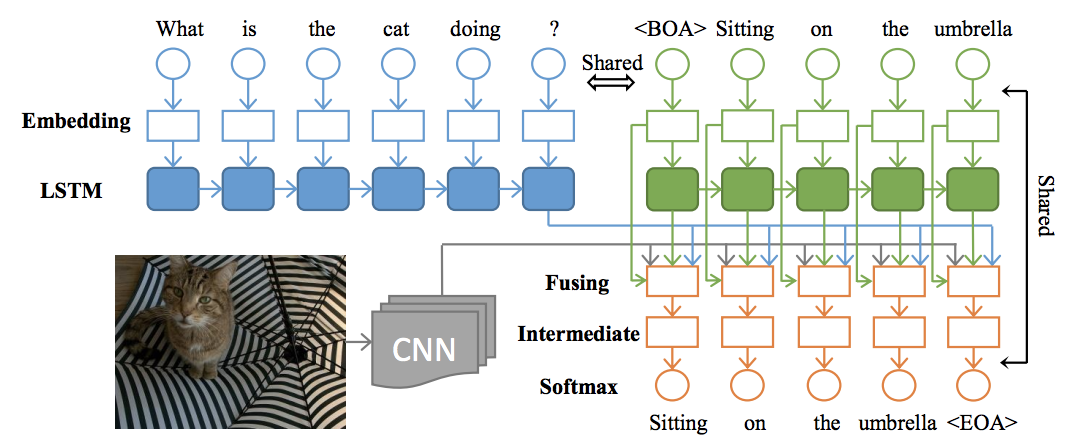
\includegraphics[width=0.8\textwidth]{mQA.png}
	\caption{mQA采用两个独立的LSTM编码问题序列和解码答案序列}
	\label{mQA}
\end{figure}

Noh等人认为单单使用相同权重参数的深度卷积神经网络去处理不同的问题,并期待能得到足够准确的答案,这是很困难的\citing{noh2016image}。因此他们提出DPPnet,在卷积神经网络CNN中添加一个动态参数层,动态参数层中的参数会根据问题的不同而改变,这使得每个问题输入都对应一个独特的分类网络。模型由三个部分组成,一个部分作为分类网络的卷积神经网络,第二个部分是参数预测网络,由门控复发单位编码问题序列,再通过一个全连接层输入动态参数,第三个部分是一个哈希函数,将参数预测网络输出的动态参数配置到分类网络中。如图\ref{DP-CNN}。
\begin{figure}[H]
	\centering
	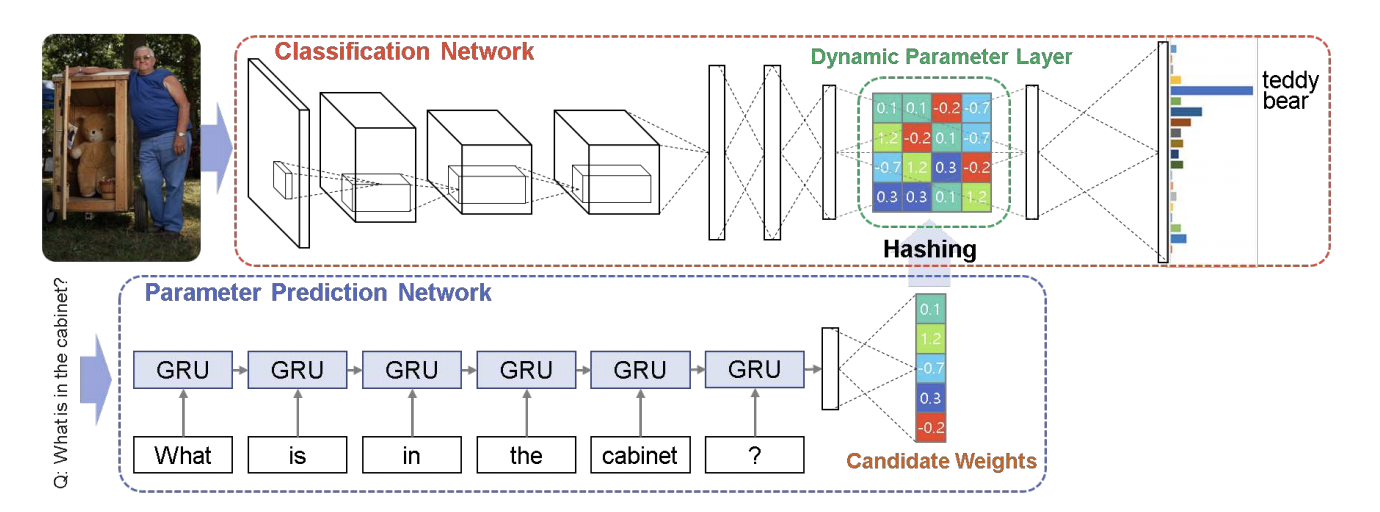
\includegraphics[width=0.8\textwidth]{DP-CNN.png}
	\caption{带有动态参数层的卷积网络模型DPPnet}
	\label{DP-CNN}
\end{figure}

Zhou等人同样适用预处理后的卷积神经网络CNN,但在处理问题文本时选择了比长短期记忆LSTM更为简单的词袋模型BOW,提出了iBOWIMG模型\citing{zhou2015simple}。iBOWIMG模型受到BOWIMG\citing{antol2015vqa}在VQA数据集上优于部分基于长短期记忆LSTM模型的启发,在原有基础上将VGGNet替换为在图像特征提取表现更优的GoogLeNet\citing{Szegedy_2015_CVPR},将图像特征向量和文本特征向量串联后送入softmax层预测问题答案(如图\ref{iBOWIMG}),在COCO-VQA数据集上的测试展现出具有竞争力的表现。
\begin{figure}[H]
	\centering
	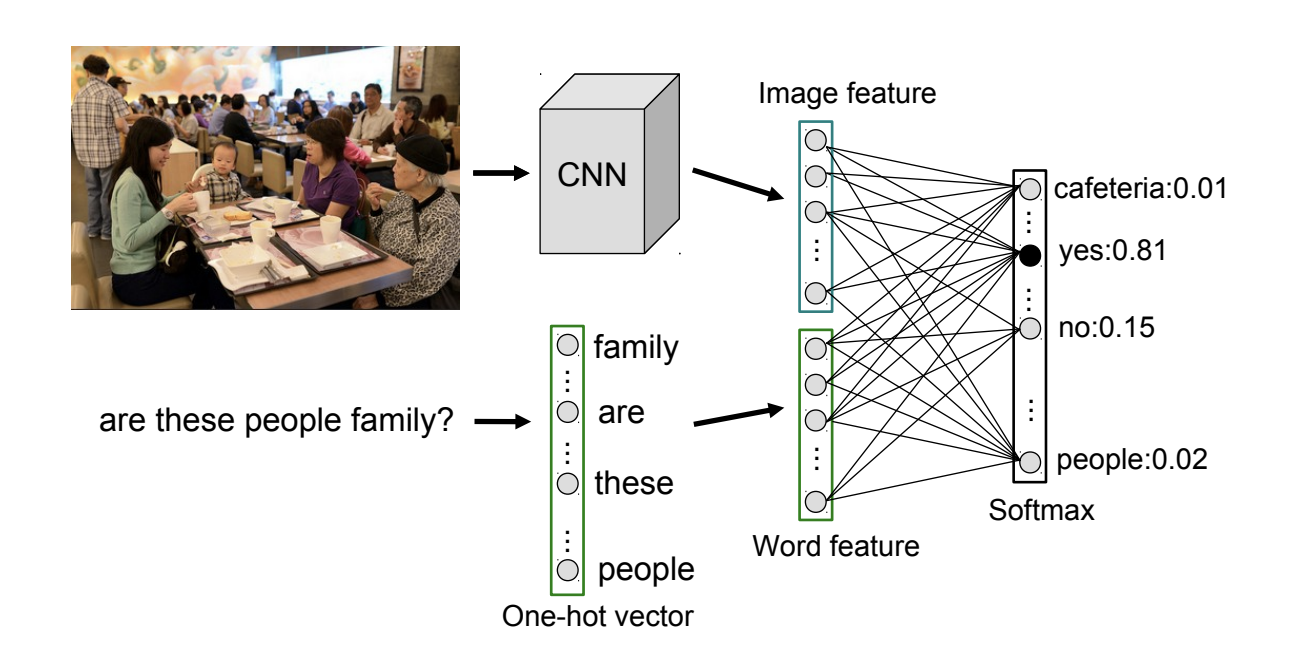
\includegraphics[width=0.8\textwidth]{iBOWIMG.png}
	\caption{iBOWIMG使用词袋BOW模型作为词特征向量编码器}
	\label{iBOWIMG}
\end{figure}

Lin等人将卷积神经网络CNN不仅应用于编码图像内容,而且也应用于问题文本的提取\citing{ma2016learning}。在处理图像特征和文本特征时使用一个多模态的卷积层输出联合特征向量,再使用softmax层预测最终的答案。如图\ref{lin}。
\begin{figure}[H]
	\centering
	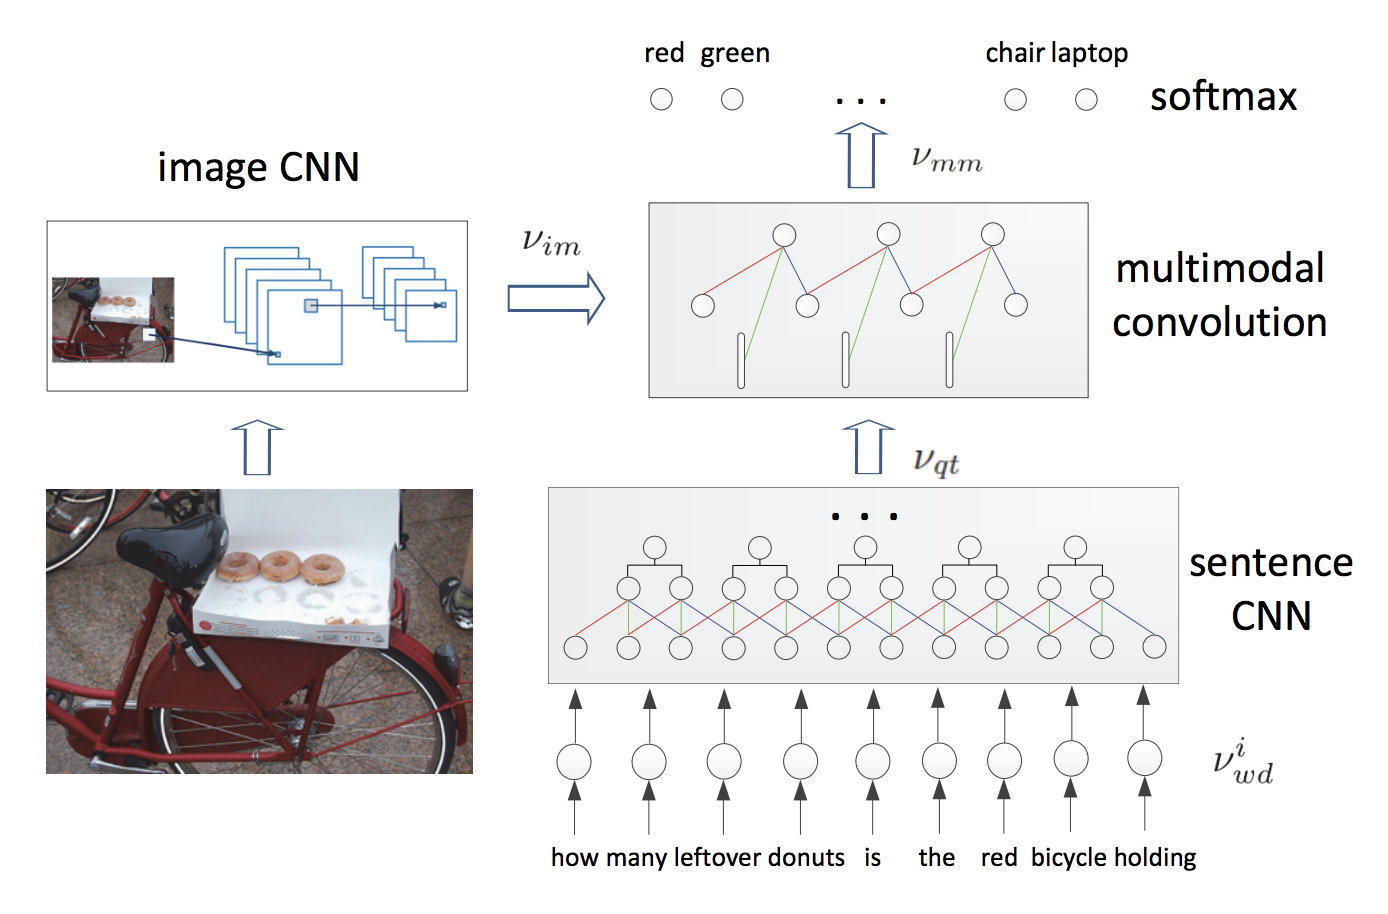
\includegraphics[width=0.8\textwidth]{lin.png}
	\caption{图像特征和问题文本特征提取时均使用CNN}
	\label{lin}
\end{figure}

除了使用不同的方法提取图像和文本特征以外,联合嵌入模型的另一个能够显著改善模型准确率的方向就是实验不用特征向量融合的池化方法。Malinowski等人通过对不同的特征向量融合方法的比较,可以看出系统的准确率与特征向量融合方法有关,不同方法之间准确率最多能相差9个百分点之多\citing{malinowski2015ask}。除了以上提到的iBOWIMG采用向量串联的方式,Lin使用向量卷积的方式外,Antol等人提出的模型使用逐元素相乘的方法融合两者\citing{antol2015vqa},Saito等人认为不同的特征融合方法各有特点,会保留或损失不同的特征,为了充分利用不同方法所保留的特征,提出了一种融合逐元素相加和逐元素相乘相结合的模型DualNet。模型同样利用了使用不同卷积神经网络CNN提取的图像特征,例如在真实场景图像采用了VGG-19\citing{simonyan2014very}、ResNet-152和ResNet-101\citing{he2016deep}。DualNet对提取出的文本特征和图像特征分别使用逐元素相加和逐元素相乘的方法得到两个不同的联合向量,再将两个的联合向量串联得到最终的合成向量,如图\ref{DualNet}。
\begin{figure}[H]
	\centering
	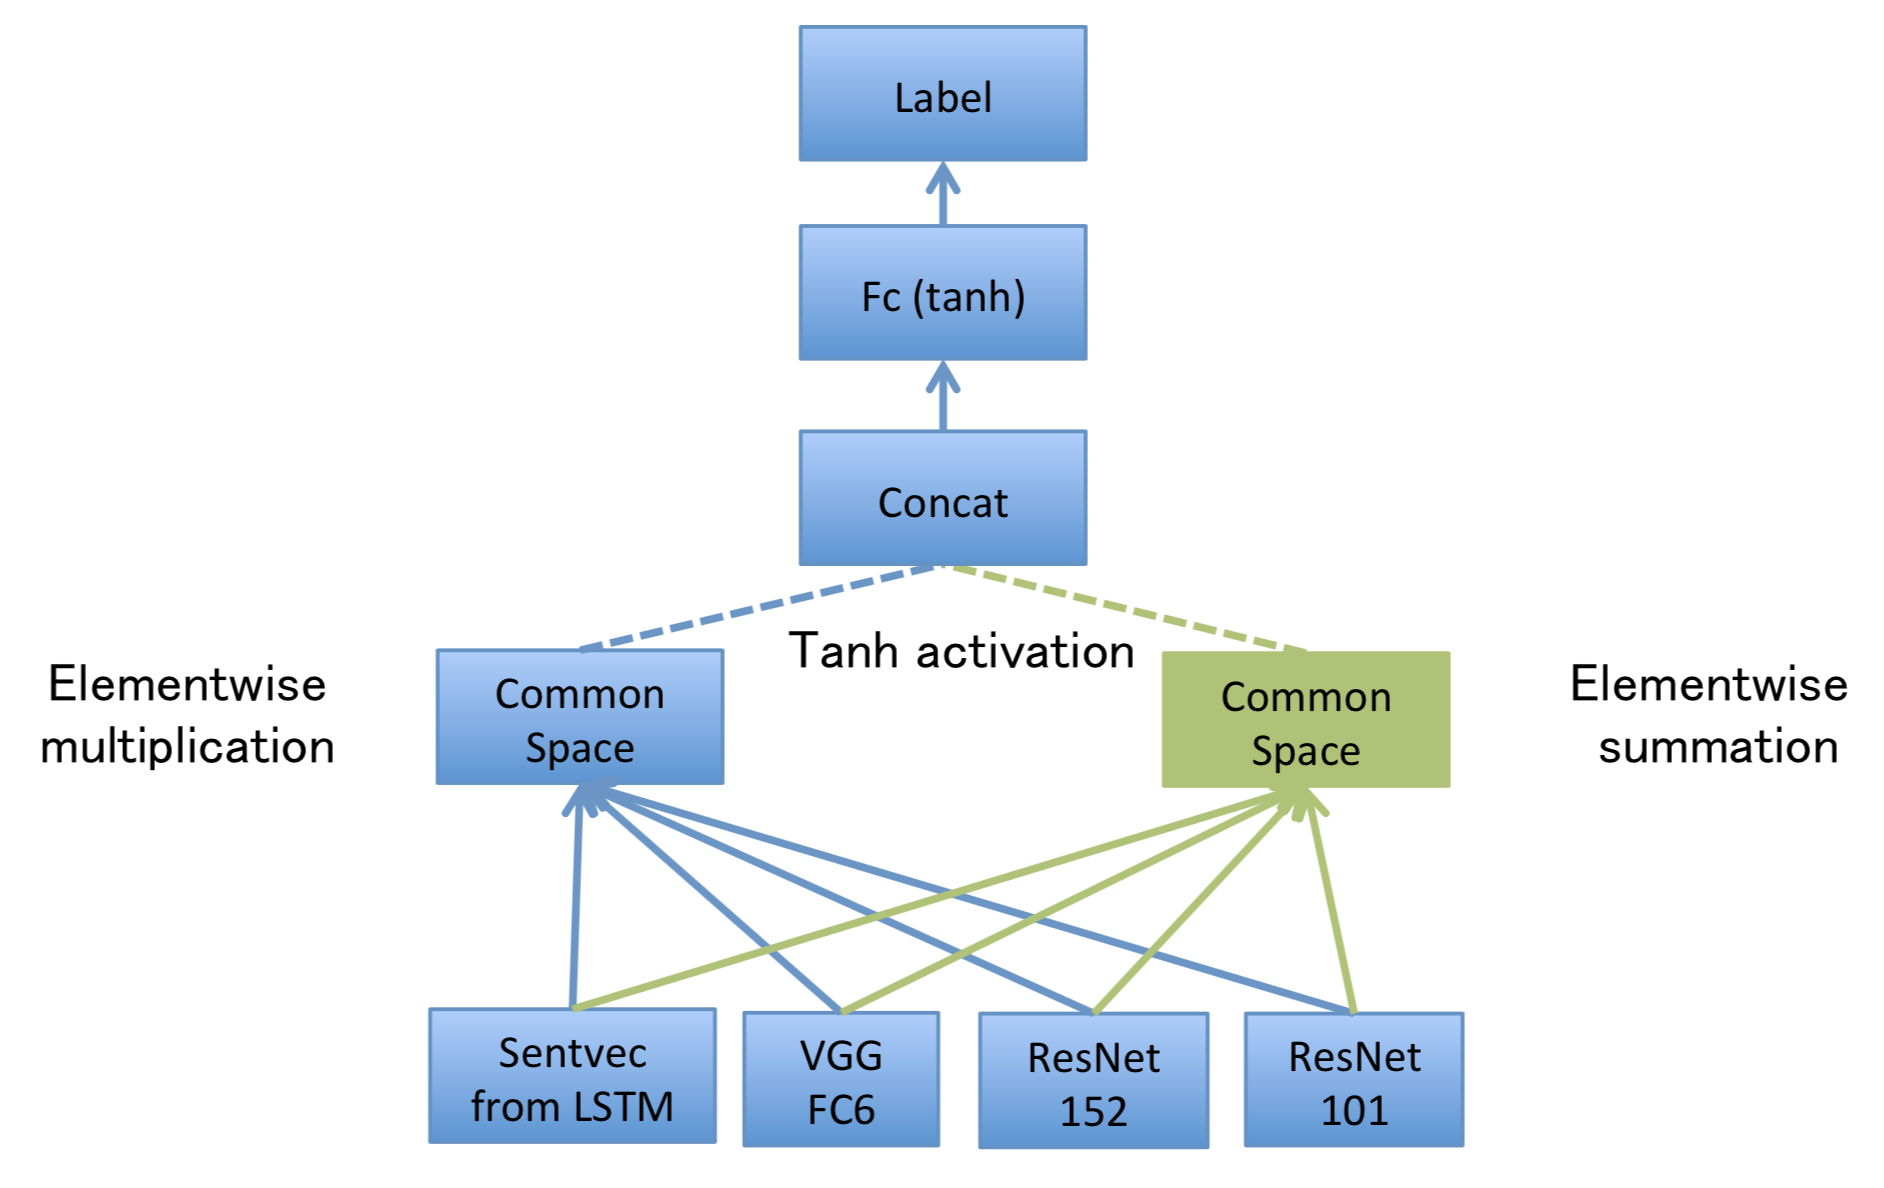
\includegraphics[width=0.8\textwidth]{DualNet.png}
	\caption{DualNet针对真实场景图像的模型架构}
	\label{DualNet}
\end{figure}

Fukui等人认为向量之间的外乘运算中,所有元素之间的互动更加活跃,应该能保留更加丰富的特征信息,因此提出一种更为复杂的多模态紧凑双线性池化方法(MCB)。一般的双线性模型会对两个向量的外乘结果线性化,外乘操作会得到异常高维的向量,例如外乘的两个向量维度均为2048、输出向量维度为3000时,那么训练参数的数量将达到125亿个之多,这会导致巨大的计算开销。而提出的多模态紧凑双线性方法能避免直接计算向量外乘,同时保留了大量特征,模型架构如图\ref{mcb}。
\begin{figure}[H]
	\centering
	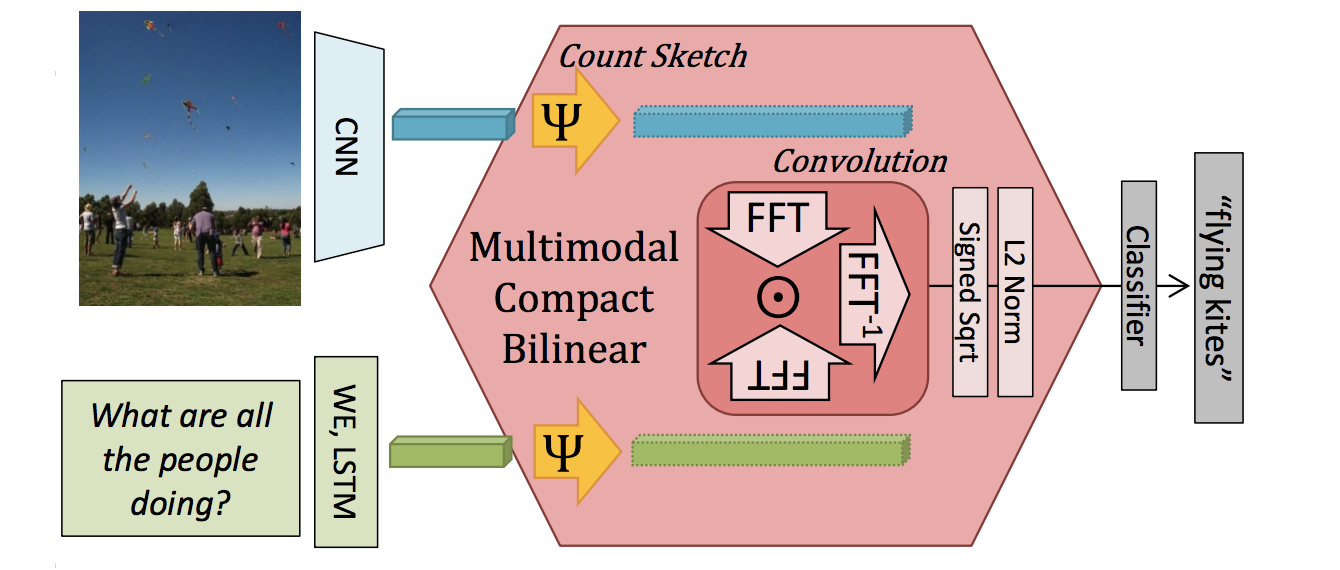
\includegraphics[width=0.8\textwidth]{mcb.png}
	\caption{使用多模态紧凑双线性池化融合图像和文本特征}
	\label{mcb}
\end{figure}

\subsection{注意力机制}
人类获取外部视觉信息时,会自动形成一种“像素不均衡”,在同一视野范围内的像素被视觉中枢神经系统根据“关注区域”的远近、相关性特征自动分配不同的分辨率,使得“关注区域”内的像素具有极高的分辨率,而其他的像素仅仅作为视觉信息输入,并不参与大脑的语义处理(如图所示\ref{human-virtual})。因此视觉注意力机制帮助大脑过滤了低相关性的视觉信息,减少了待处理数据的体积,极大地提高了信息处理速率并松弛了大脑负载。
\begin{figure}[H]
	\centering
	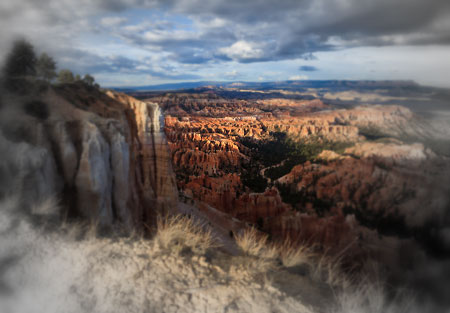
\includegraphics[width=0.5\textwidth]{human-virtual.png}
	\caption{人类视觉系统的“像素不均匀”现象}
	\label{human-virtual}
\end{figure}

近几年,受到人类视觉注意力机制的启发,在神经网络中引入注意力机制变得十分热门,在自然语言处理和计算机视觉领域的应用也极大得帮助了原有算法精度和计算效率的提升。Google Deepmind团队提出了一种带有注意力机制的循环神经网络(RNN),并成功应用于图像分类任务,获得了优于以往卷积神经网络(CNN)的基线水平的分类精度\citing{mnih2014recurrent}。随后,带有注意力机制的循环神经网络便被广泛应用于自然语言处理和计算机视觉的多个子领域\citing{bahdanau2014neural, xu2015show, NIPS2015_5847}。Bahdanau等人将注意力机制引入神经机器翻译任务,仍然使用“编码-解码”的翻译模式,但一改以往将源语言文本映射为一个固定长度的向量的编码方式,而是将原语言文本编码为向量序列,解码时将翻译和位置对应因素联合学习,训练向量序列中各向量对翻译词组的不同权重,加和完成翻译结果的推断,得到了以往最优的结果\citing{bahdanau2014neural}。Xu等人受到注意力机制在机器翻译和物体识别任务成功应用的启发,将带有注意力机制的循环神经网络应用于自动生成图片说明,并且在Flickr9k, Flickr30k 和MS COCO 三个数据集上均获得了最优的结果\citing{xu2015show}。随后,更多注意力机制的变型或优化研究均在图片说明任务上展开\citing{ 7243334, wu2017global, li2017image, lu2017knowing}。

相较起图片说明任务,视觉问答任务除了要求系统能理解图片内容,生成语义和句式合理的自然语言文本以外,还需要联合学习问题文本和聚焦与问题相关的图像细节。这些任务特性决定了视觉问答任务可以利用已有较为先进的图片说明任务的框架,同时融合自然语言处理的最新成果。注意力机制在自然语言处理和计算机视觉上的成功应用便成为了视觉问答算法快速发展的基石。

Chen等人最先将注意力机制引入视觉问答任务,提出了基于注意力机制的可配置卷积神经网络(ABC-CNN)用于针对“图像问题对”生成对应的注意力映射,将问题的语义信息和图像区域建立映射,使得答案生成取决于被关注区域,减少无关区域的影响\citing{chen2015abc}(模型架构如图\ref{abc-cnn})。在Toronto COCO-QA\citing{ren2015exploring}, DAQUAR\citing{ malinowski2014multi}, 和VQA\citing{antol2015vqa}三个数据集上的测试结果都提升了最优结果,证明了注意力机制在提高视觉问答任务上的有效性,同时注意力权重图能反应系统的推理过程,为参数的微调提供了依据。
\begin{figure}[H]
	\centering
	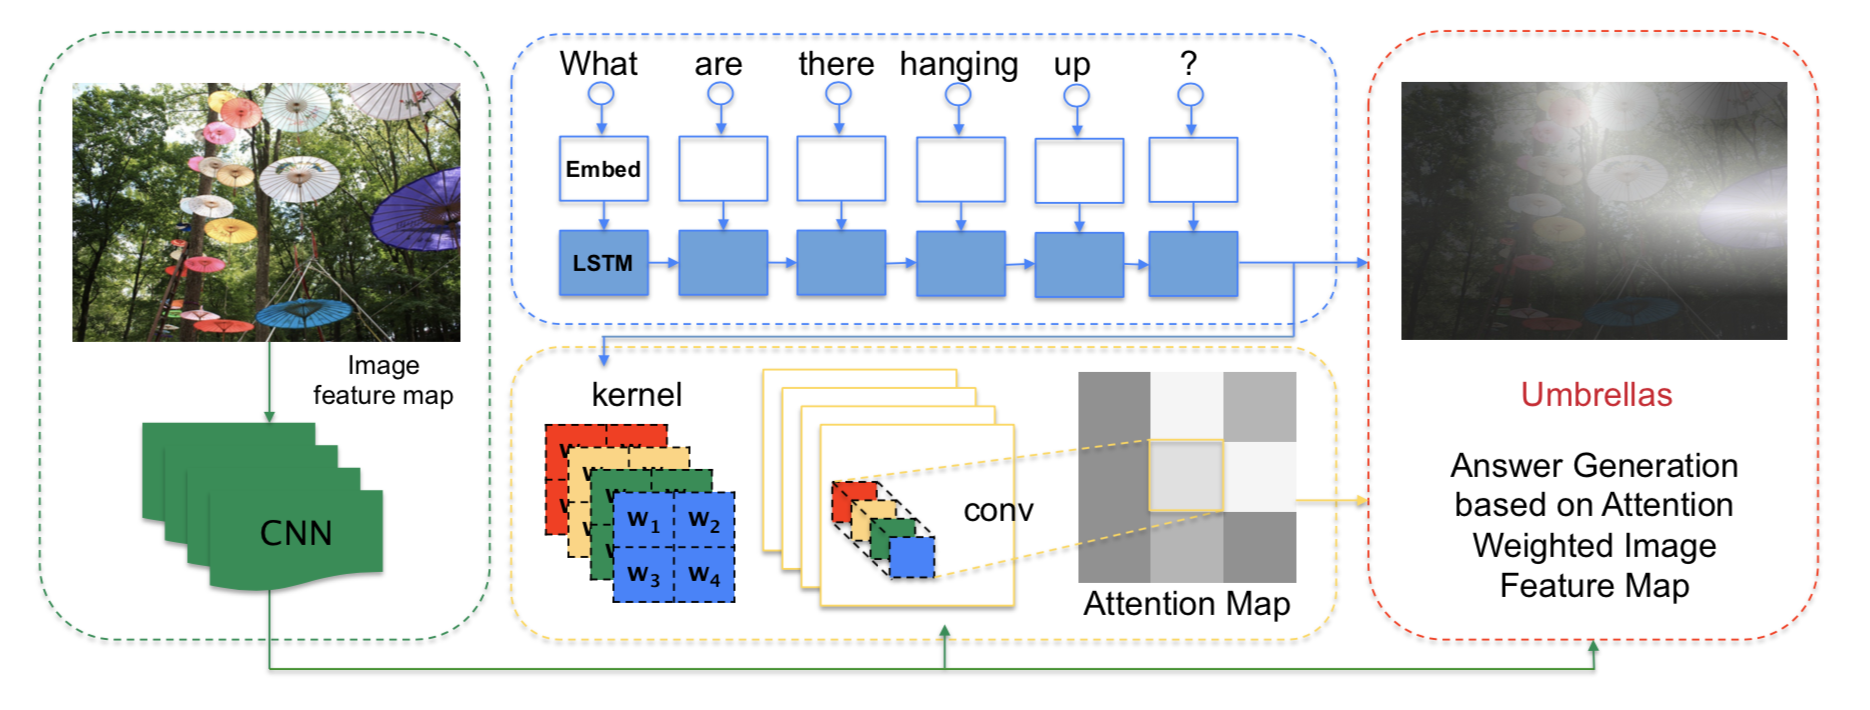
\includegraphics[width=0.8\textwidth]{abc-cnn.png}
	\caption{ABC-CNN使用CNN提取图像特征,LSTM提取问题文本特征,黄色方框内为用于推测与问题相关的图像区域的注意力机制}
	\label{abc-cnn}
\end{figure}

Shih等人使用简单的word2vec方法编码“问题-答案”对,使用预处理后的卷积神经网络CNN对图片的不同区域编码,将编码后的文本特征向量和图片特征向量映射到同一特征空间,根据特征之间的点乘运算决定每个图像区域的权重,最后结合权重化以后的图像特征和文本特征得出答案。架构如图\ref{shih}。在辨别物体颜色的任务上得到了最优结果\citing{ shih2016look}。类似的工作还有Ilievski等人提出的“聚焦型动态注意力模型“\citing{ilievski2016focused}。
\begin{figure}[H]
	\centering
	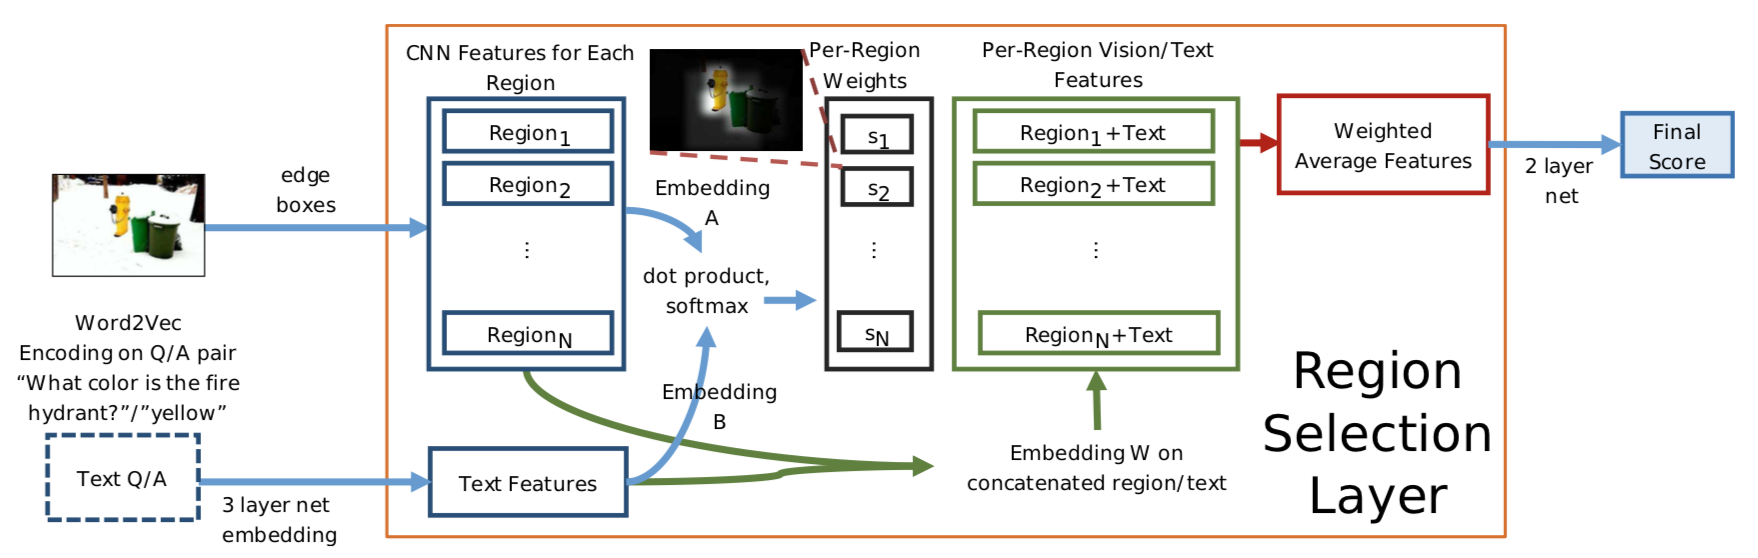
\includegraphics[width=0.8\textwidth]{shih.png}
	\caption{使用图片区域选择层实现注意力机制的架构}
	\label{shih}
\end{figure}

包括以上提到的在内,多数注意力机制对问题文本和图像区域特征进行一次运算,直接生成图像注意力权重图。针对这种情况,Yang等人提出堆栈式注意力网络——使用问题的语义表达对图像进行多次查询,不断缩小答案相关区域,实现更高的精度\citing{yang2016stacked}。注意力机制在视觉问答上的其他应用还有,同时使用对图像和问题使用注意力机制的联合注意力模型\citing{NIPS2016_6202};不采用图像区域赋值方法,而是过滤掉不相关区域的“自适应硬性注意力网络”\citing{malinowski2018learning}。

对于神经网络训练这类参数密集和计算密集的框架,注意力机制能带来两个重要的改变。一方面,无论对于图像输入还是文本输入,原有的方法都选择将输入看做一个整体,因此映射后的向量需要包含完整的输入信息,对于包含词组过多文本或是场景过于复杂的图像,编码后的向量根本无法区分开输入的局部特征,这使得神经网络的可解释性大大降低。引入注意力机制后,编码方式改变,将输入视为为局部信息的综合,保留了文本中单词和图像中像素区域的信息,通过可视化处理,能清晰的看出神经网络的推理过程,增强了系统的可解释性,可以称之为一种“弱化黑盒的处理”。另一方面,注意力机制非常符合人类对于语言和视觉信息的处理方式,这背后的假设是:针对绝大多数任务,只需要从信息源的局部便能获得充分正确的答案。类似于人类,具有注意力机制的智能体应当能获得更高的执行的效率和更高的答案精度。

\subsection{动态记忆网络}
无论是在自然语言理解还是图像内容理解,人类在获取单词或者图像像素区域的语义时不会将其与语境割裂来看,通常上下文语境对于准确理解文本和图像信息是非常重要的,因为在语言和图像中存在大量具有歧义特性的内容,例如,在语言中一个单词具有不同的语义,也可能有不同的词性,只有在上下文的语境中才能确定词语的真正含义。记忆力与上下文语境相似,是神经网络在训练过程中存储的“经验”,这种“经验”有助于以后的训练,这种累积经验能创造更准确的答案,基于这样的假设,研究人员为从序列化的输入中获得更准确的输入,而引入了动态记忆网络\citing{jiang2015compositional,kumar2016ask,xiong2016dynamic}。

Jiang等人在常见的CNN解析图像、LSTM解析问题文本的架构上,新增一个成分记忆模块\citing{jiang2015compositional},旨在融合每一次训练过程中的局部图像信息和文本信息,并提供给下一次训练使用,从而使网络存储了训练过程的“经验”,这与之后提出的动态记忆网络有同样的思想,模型训练流程如图\ref{c-memory}。
\begin{figure}[H]
	\centering
	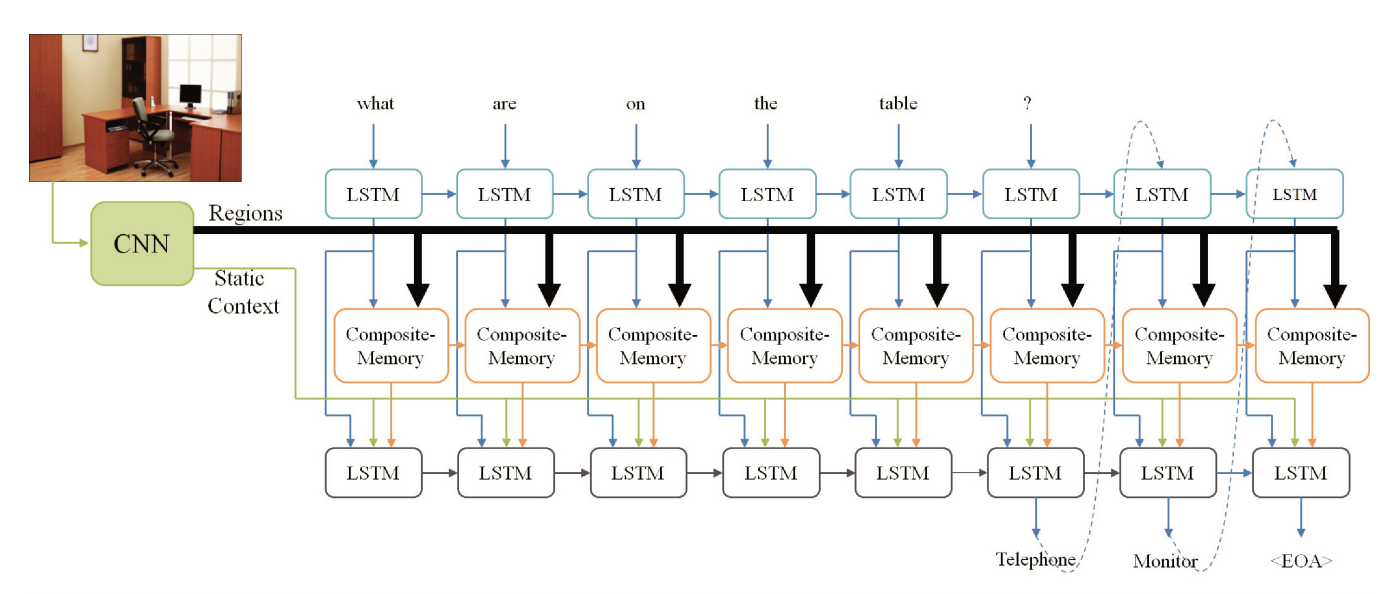
\includegraphics[width=0.8\textwidth]{c-memory.png}
	\caption{成分记忆模型的训练流程}
	\label{c-memory}
\end{figure}

Kumar等人为解决文本问答(Text-QA)任务而提出动态记忆网络(DMN)\citing{kumar2016ask}。动态记忆网络(DMN)是一个用于生成文本问题答案的神经网络框架,它由输入模块、问题模块、情节记忆模块和问题模块构成,输入模块用于编码文本输入;问题模块用于编码文本问题;情节记忆模块接受由输入和问题模块得到的分布式向量,再使用注意力机制选择部分接受到的向量,结合选择后的向量与以往存储的“记忆”生成新的“记忆”向量,并不断迭代;答案模块根据最终的记忆向量生成答案,模型架构如图\ref{dmn}。
\begin{figure}[H]
	\centering
	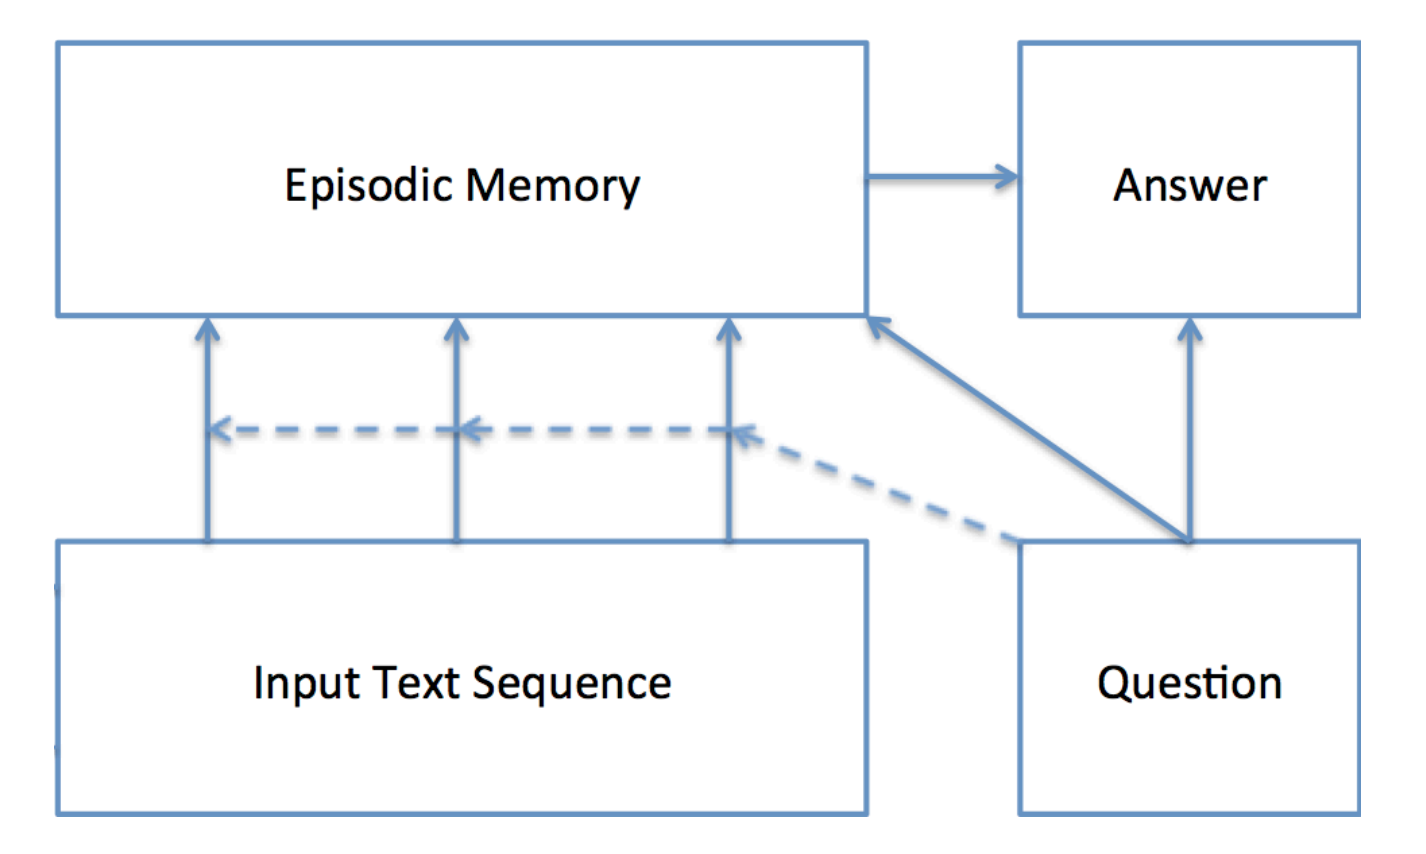
\includegraphics[width=0.5\textwidth]{dmn.png}
	\caption{DMN基础架构}
	\label{dmn}
\end{figure}

动态记忆网络(DMN)在文本问答、语义分析、词性标注任务上取得了最优的结果,受到其在处理序列化的文本信息上的优异表现的启发,Xiong等人在原有网络的基础上改善了输入和记忆模块,除了能处理文本信息外,还能处理图像信息,提出应用到于视觉问答任务动态记忆网络+(DMN+)\citing{xiong2016dynamic},如图\ref{v-dmn}。动态记忆网络+(DMN+)将原有的输入模块中处理文本编码的门控复发单元(GRU)更换为双向门控复发单元(bi-GRU)以得到文本或图像区域更完整的上下文信息;使用基于注意力机制的门控复发单元替换原有的软性注意力机制。更新后的动态记忆网络+(DMN+)在DAQUAR\citing{malinowski2014multi}和VQA数据集\citing{antol2015vqa}上的测试结果都得到了具有竞争力的表现。
\begin{figure}[H]
	\centering
	\subfigure[应用于文本问答的动态记忆网络(DMN)模型架构]{
		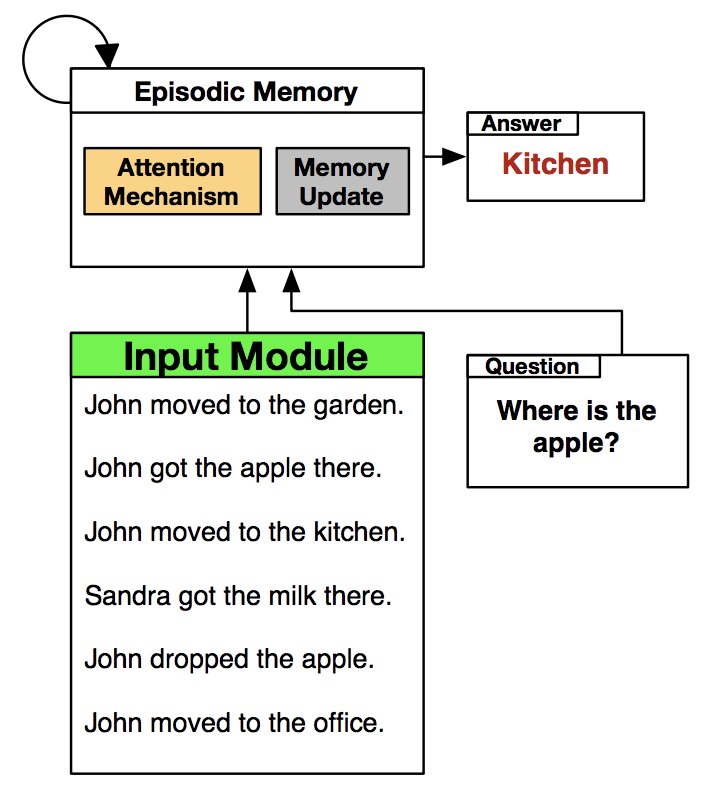
\includegraphics[width=0.4\textwidth]{t-dmn.png}}
	\subfigure[应用于视觉问答的动态记忆网络+(DMN+)模型架构]{
		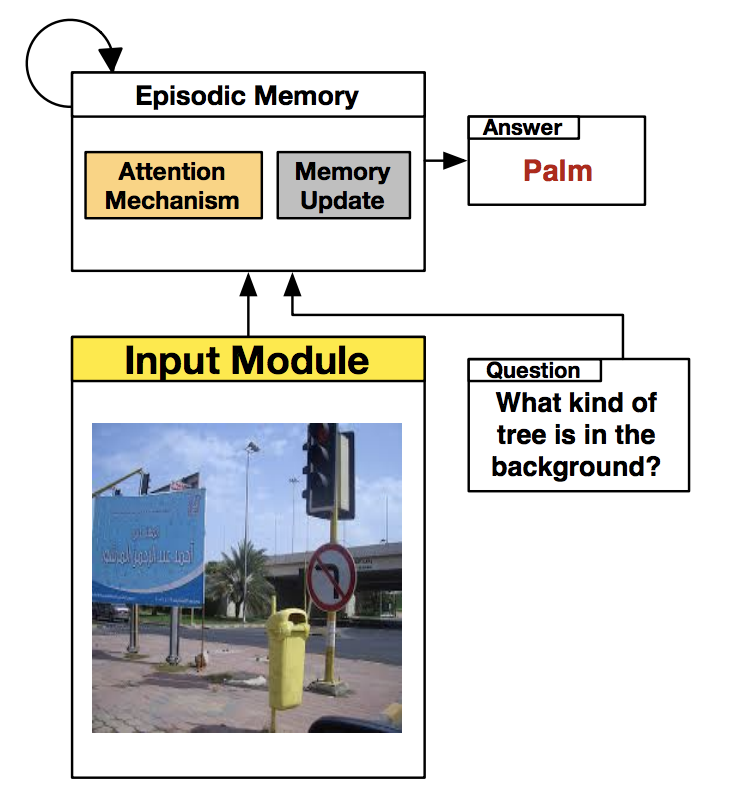
\includegraphics[width=0.4\textwidth]{v-dmn.png}}
	\caption{DMN+与DMN架构对比}
	\label{v-dmn}
\end{figure}

\subsection{基于外源知识库的视觉问答算法}
视觉问答任务基于图像场景回答问题,图像理解、问题理解和答案生成是实现准确的视觉问答系统的算法核心。图像理解、问题理解和答案生成三者又可以根据人类思考逻辑将其划分为两个逻辑层次,问题理解成为逻辑基点,图像理解和答案生成都根据问题的不同而采用适当的算法策略——注意力机制便是一种借助问题理解而实现计算效率更高的图像解析方法,答案生成中关心的答案类型和答案词组长度也需要依照问题的不同而选择。因此问题的解析过程对于视觉问答算法的准确性和计算成本都有很大的影响。

正如绪论中提及的,问题可以分为识别和推理两个大类,推理任务中既要求系统能准确识别图像中的对象,往往也会涉及图像中无法获取的先验知识。先验知识包括众所周知但不会显性呈现的常识和面对特定领域需要具备的专业知识,例如,判断路口是否可以通行时,涉及基本交通规则的常识,判断艺术品的作者这类专业问题时,需要借助与该艺术品相关的知识储备。

先验知识对视觉问答系统提出了更高的要求,这也揭露了主流的联合嵌入模型的缺陷:第一点,联合嵌入模型的答案生成来源于训练集中的问题和答案文本,这意味着训练集中包含的知识和文本内容是整个视觉问答系统的所有知识来源,因此对于测试集中涉及的全新概念或答案,系统根本无法得出正确的答案。不断扩充包含更多先验知识的训练集是提高精度的方式之一,但对于整个世界蕴含的不可计量的知识而言,这种数据集扩充的方式成本巨大。第二点,联合嵌入模型要求网络本身能存储学习到的知识,目前网络的容量相较于需要学习的知识是严重不足的。第三点,神经网络海量参数和复杂网络连接带来的黑盒特性依然存在。对于识别和分类等问题而言,可解释性与高精确度相比,显得不那么重要,但是对于需要明确推理过程的问答系统而言,黑盒的不可解释性会降低提问者对系统的可信度,毕竟没人会轻易相信一个无法解释的答案。

一种可行的解决方案是将推理过程和知识学习分离,保留系统原有的图像理解和问题文本理解模块,在答案生成模块中引入外源知识库。可扩展的外源知识库可以解决网络容量的限制问题;知识库中结构化的数据可以作为推理过程的起点,知识库中的数据关联能为推理提供路径,形成逻辑链条,提高系统的可解释性。本节将对已有的基于知识库的视觉问答方法进行详细的介绍,分析各种方法的优势和存在的问题。

\textbf{Ahab}

Wang等人提出的Ahab视觉问答系统利用DBpedia作为知识库,实现对需要先验知识的问题的推理应答,即使问题中涉及不包含于图像中的概念\citing{wang2015explicit}。Ahab的主要思路为三点,第一点,将图像中的概念链接到知识库中相同的概念,形成从图像到知识库的映射,第二点,将自然语言的文本问题处理为知识库查询语句,实现从自然语言的句法和语义结构变换到相应的查询语句结构,第三点,将知识库的查询结果转换为自然语言表达。利用以上三点,Ahab可以不通过数据集训练获取知识,而使用自然语言到知识库的两次转化完成问答任务。

具体来说,为了建立图像概念到知识库实体之间的映射,首先检测图像包含的概念,再将提取出的图像概念和知识库实体建立链接。Ahab从图像中提取物体对象、图像场景和图像属性三种视觉概念,对象提取使用在MS COCO\citing{lin2014microsoft}和ImageNet\citing{deng2009imagenet}上预训练后的Fast-RCNN\citing{ren2015faster},能实现224种类型的对象识别;场景分类器使用预处理于MIT Places205\citing{zhou2014learning}数据集的VGG-16 CNN,理论上能实现对205种场景的识别,每张图片选取分数前三的场景标签;图像属性提取器使用预处理于ImageNet\citing{deng2009imagenet}和MS COCO\citing{lin2014microsoft}的VGG-16 CNN,每张图片选取分数前十的属性标签。所有提取出的图像信息都使用资源描述框架(RDF)的形式表示,例如,“图像中包含长颈鹿对象”被表示为(图像,包含,对象1),(对象1,名称,长颈鹿)。每个视觉概念则被直接链接到具有相同语义的知识库概念,如图所示\ref{linkingMathord}。
\begin{figure}[H]
	\centering
	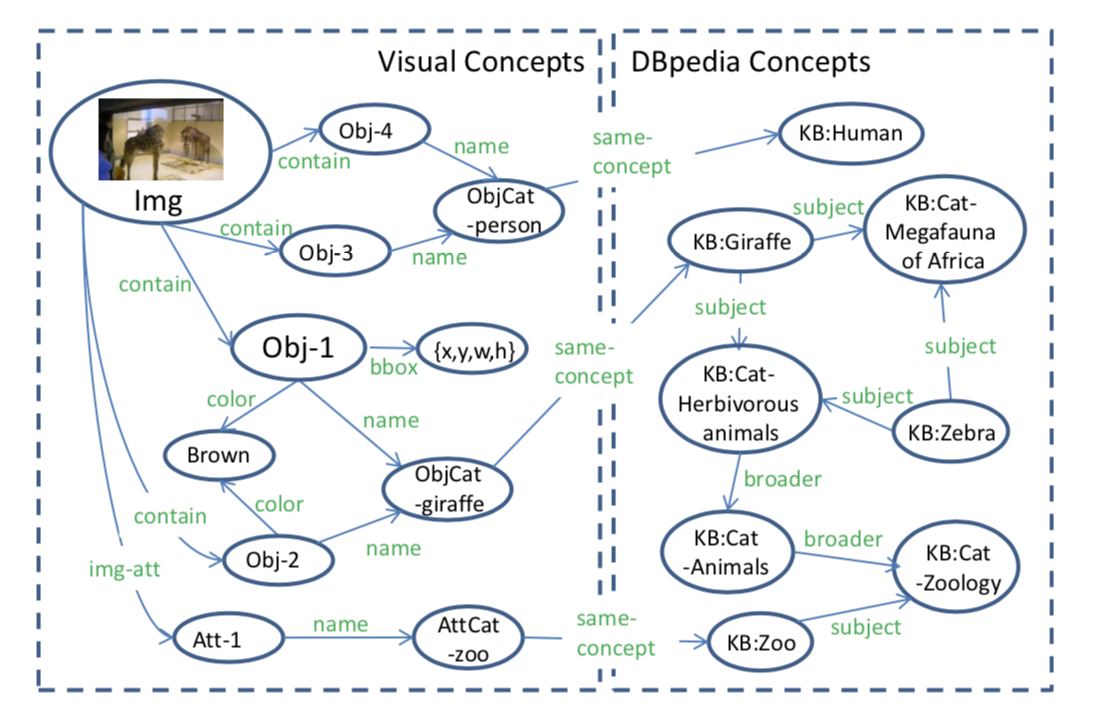
\includegraphics[width=0.8\textwidth]{linkingMathord.png}
	\caption{Ahab中链接图像信息和知识库实体的RDF图结构}
	\label{linkingMathord}
\end{figure}
所有资源描述框架(RDF)数据被存储在OpenLink Virtuoso中——一个能存储多种数据类型的数据库。

Ahab使用Quepy开源框架将自然语言问题转化为相应的知识库查询语句,但Quepy解析问题时,需要预先设定的正则表达式模板,因此Wang等人使用KB-VQA数据集作为实验数据集。结合KB-VQA中的23种问题模板和针对不同问题类型的谓语选择,Ahab能根据不同的问题产生相应的查询语句,并得到问题答案。

Ahab类似于专家系统,针对特定的问题设定了与之对应的知识库查询方法,应用于知识库的搜索路径可以为视为系统“逻辑推理”的过程,因此Ahab不仅输出最终的答案,而且也将答案推理的过程作为输出,实现了对系统推理的显性表达,问题处理的过程如图\ref{question_processing}。
\begin{figure}[H]
	\centering
	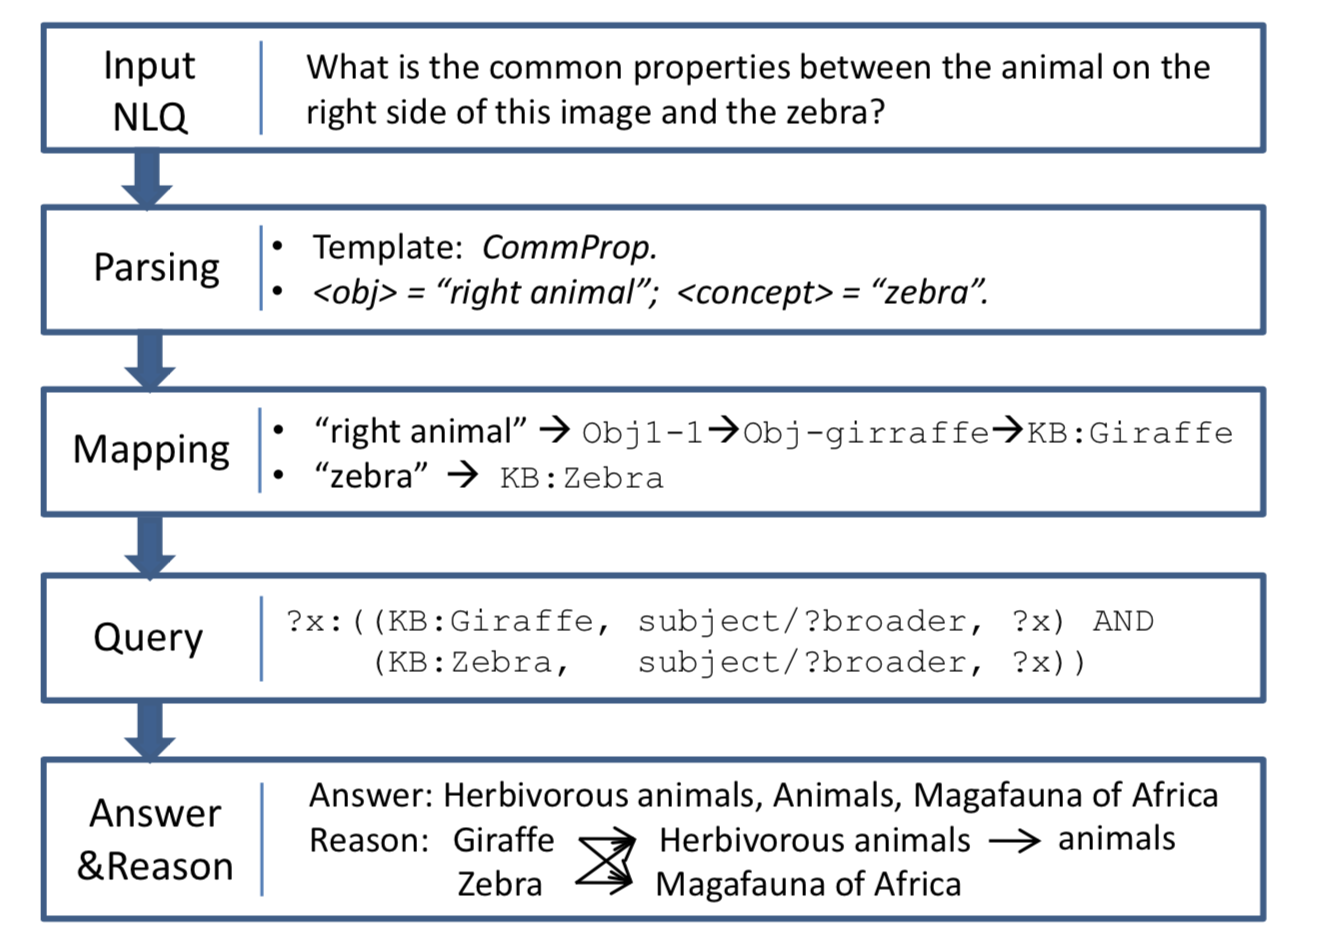
\includegraphics[width=0.8\textwidth]{question_processing.png}
	\caption{Ahab结合问题文本和预先设定的模板,解析出问题中的概念,再将问题中的概念与知识库实体建立链接,并生成查询语句,得到查询结果和推理过程}
	\label{question_processing}
\end{figure}

在评估Ahab对于需要先验知识的问题的表现时,Wang等人使用了自己构建的KB-VQA数据集(上文中有详细介绍)作为测试集,但KB-VQA中的问题多数是开放性的,并且还没有自动化评估正确性的方法被提出,因此使用人工的方式对结果的正确性进行评估,每个结果被人工地赋予5种表示正确程度的分数:1分-完全错误、2分-部分错误、3分-模棱两可、4分-基本正确、5分-完全正确。

作为对比,评估还引入了由人类作答和主流的联合嵌入模型作答两种方式——使用CNN编码图像特征,LSTM编码问题文本和生成答案的模型,三种测试系统在不同问题的正确率和平均得分如图\ref{ahab_evaluation}。
\begin{figure}[H]
	\centering
	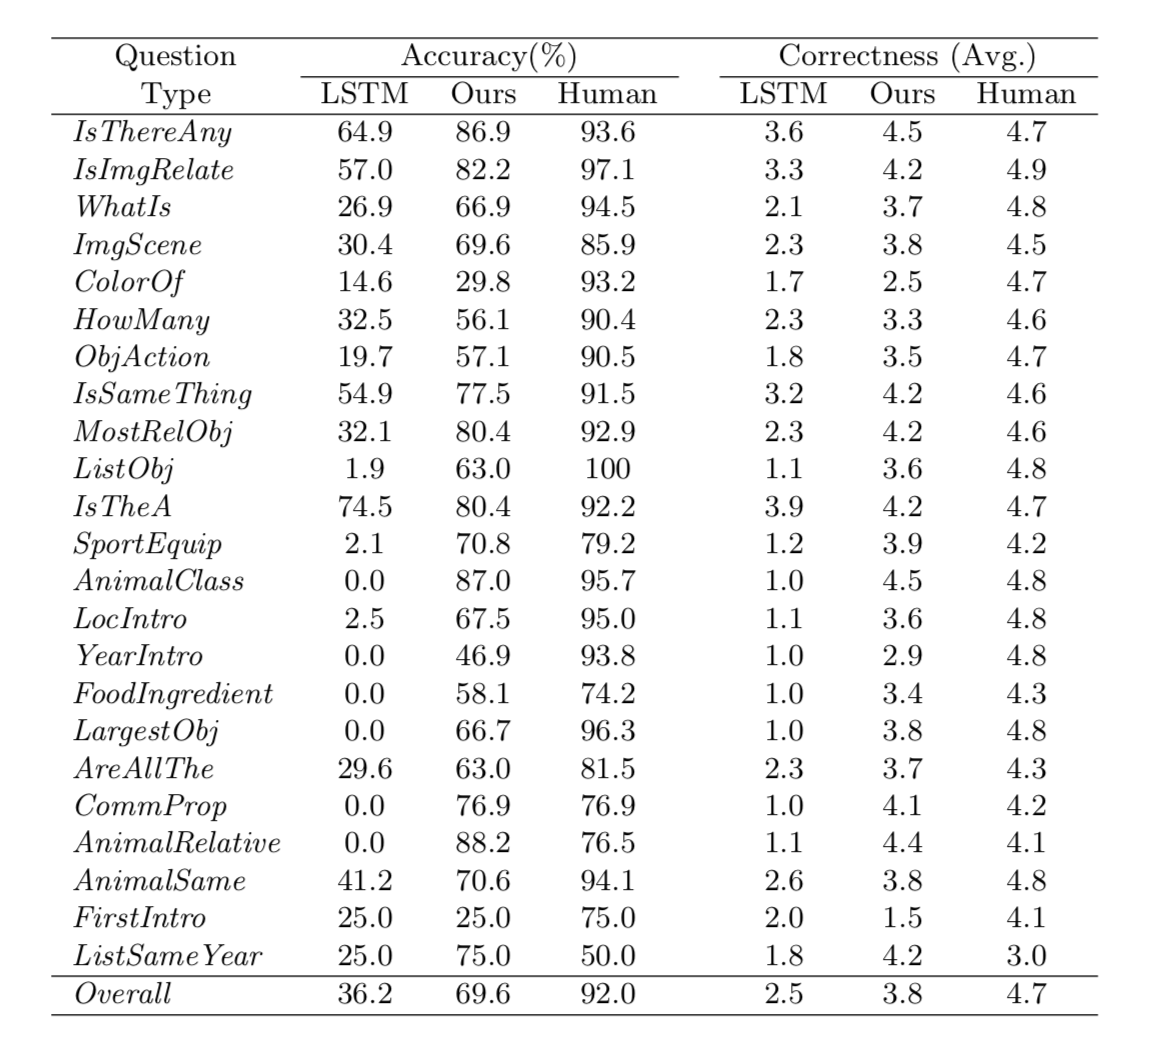
\includegraphics[width=0.8\textwidth]{ahab_evaluation.png}
	\caption{Ahab、联合嵌入模型和人类作答在23种问题上的表现。Accuracy是得分超过3的问题数量的比例,Correctness是某类问题得分的加权平均数。}
	\label{ahab_evaluation}
\end{figure}
KB-VQA将23种问题类型划分为“视觉问题”、“常识问题”、“知识库问题”三个知识等级,如图\ref{qtd},三种不同方法在三种知识等级的正确率统计如图\ref{type_evaluation}。
\begin{figure}[H]
	\centering
	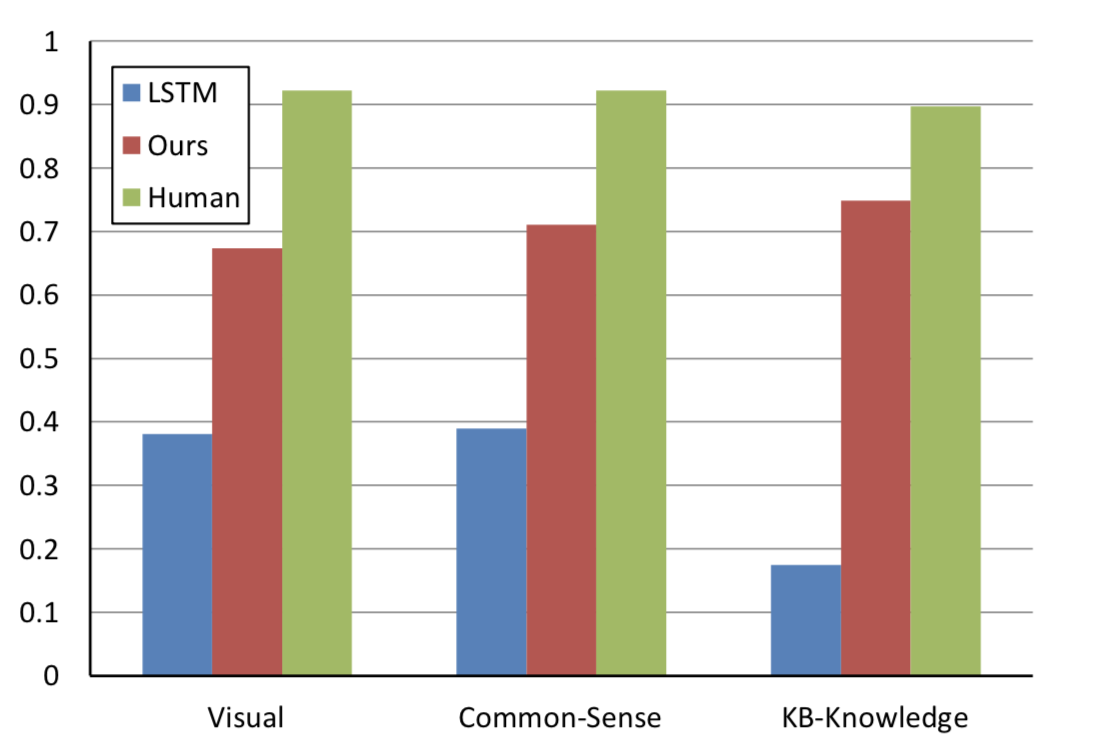
\includegraphics[width=0.8\textwidth]{type_evaluation.png}
	\caption{三种不同方法在三种知识等级的正确率统}
	\label{type_evaluation}
\end{figure}

从图\ref{qtd}中可以看出,LSTM的联合嵌入模型在“判断动物类别”、“判断对象生产年份”、“列出不同对象的共同属性”、“列出食物营养成分”、“判断最大/最小的物体”、“列出动物的近亲”这六种任务中正确率为0,其中除去“判断最大/最小的物体”为视觉问题外,其余5种问题均需要系统结合额外的知识回答,这正是基于训练集的概率模型的劣势——对于复杂关系和长知识链条的学习能力。总体上看,Ahab在每种问题类型上都优于联合嵌入模型,但离人类的正确率还是有一定差距,尤其在“判断物体颜色”和“比较两个物品的诞生先后”两种问题。

对于“列出与某个物品相同年份的物品”这类问题上,Ahab以75\%的准确率高出人类的50\%,但值得注意的是,KB-VQA数据集中此类问题只有4个,也就是说Ahab只是比人类多答对一个问题,考虑到答案生成过程和正确性评估过程中可能产生的误差,这并不能肯定的表明Ahab系统在此类问题上优于人类的表现。同样的状况也出现在其他问题类型上,因此KB-VQA在不同问题类型上数量的不均衡(问题数最多的类型与问题数最少的类型数量相差两个数量级)和问题样本数过小(16种问题类型的数量小于100,其中有两种的问题数量小于100)在评估视觉问答系统的真实推理能力上不能产生置信度足够高的结果,丰富数据集的样本和均衡不同类型的样本数量才能更好得评估系统的推理表现。

除了测试集存在稳定性较低和样本数较少的问题以外,Ahab系统只能针对预先设定的23种问题类型,这大大限制了问题的开放程度,不能满足真实的问答环境中海量的问题类型。而且Ahab的高正确率还建立在针对性地生成不同的问题查询语句之上,当问题类型数量剧增时,人工的对每种类型设定对应的算法是不切实际的,因此Ahab系统的扩展性也面临挑战。

但相较于主流使用统计方法的联合嵌入模型,Ahab利用知识库取代知识学习过程的方法在复杂推理任务,尤其是需要运用先验知识的问题上,实现了更好的系统表现,也为解决复杂推理问题的方法上提供了有益的实践。

\textbf{FVQA}
Ahab将问题解析为知识库查询语句时,需要预先确定问题模板,这极大的限制了系统面对多样化问题的能力,因此Wang等人改变了问题到查询语句的映射方式提出了FVQA模型\citing{wang2017fvqa}。FVQA模型使用带有FVQA数据集,FVQA数据集中的数据格式为(图片,问题,答案,支持事实),支持事实是一个包含答案的资源描述框架(RDF)数据,例如,(猫,能,爬树)。FVQA数据集中的问题包含三个属性:视觉概念(包含物体对象、场景和行为三种类型)、谓语(12种类型)和答案来源(图像和知识库两种)。FVQA模型在训练阶段,从标注后的支持事实中提取出问题的三种属性(VC表示视觉概念类型、REL表示谓语类型、AS表示知识来源类型),由于FVQA数据集中三种属性之间的组合能形成28类问题,所以FVQA模型使用长短期记忆(LSTM)网络训练一个28类的查询语句分类器,实现将问题到查询语句的分类过程,28种查询类型及其在训练/测试集的分布如图\ref{fvqa_query}。
\begin{figure}[H]
	\centering
	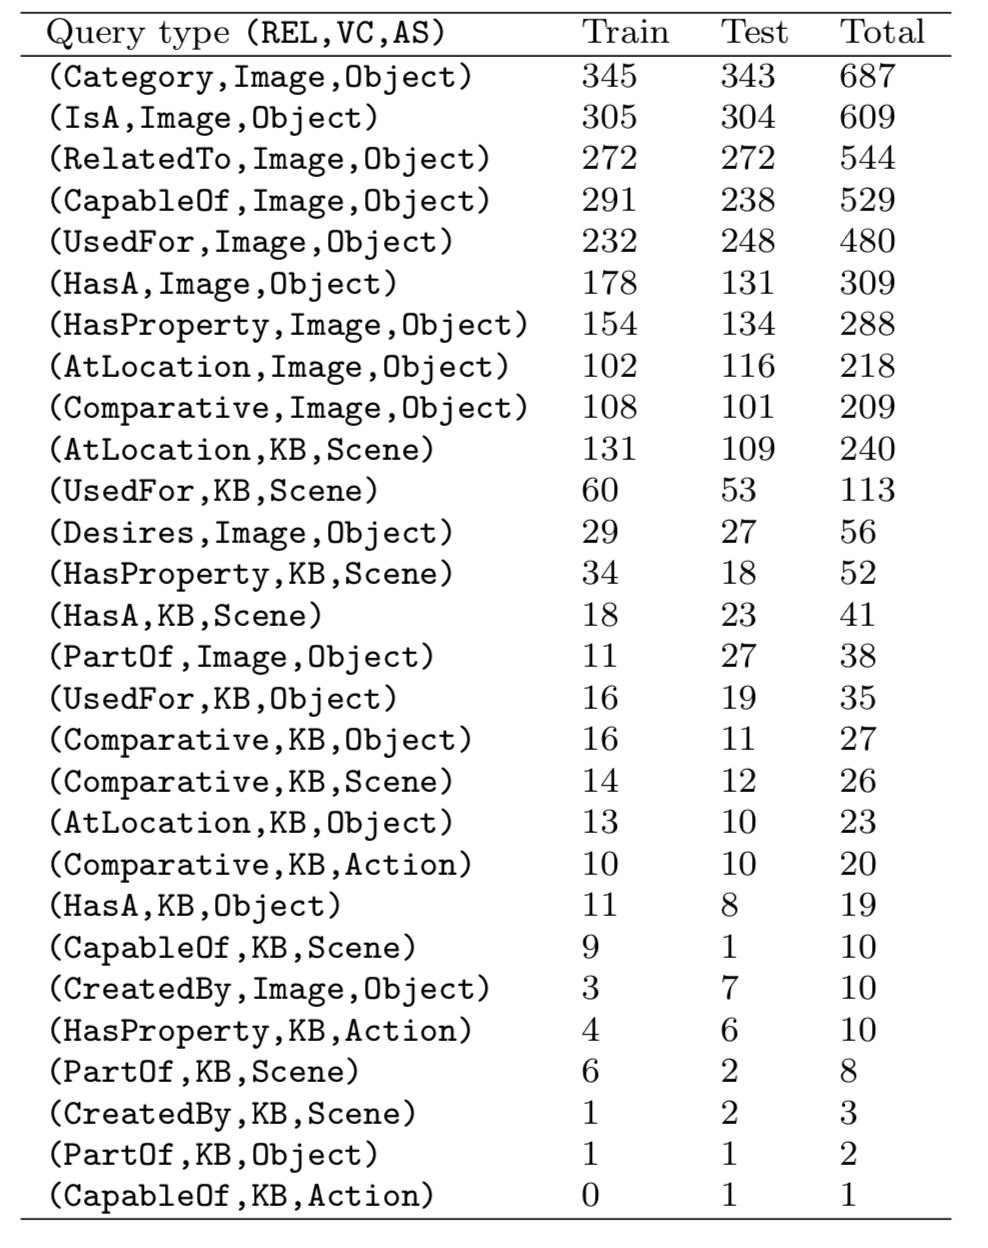
\includegraphics[width=0.5\textwidth]{fvqa_query.png}
	\caption{FVQA模型的28种查询类型及其在训练/测试集的分布情况}
	\label{fvqa_query}
\end{figure}

通过LSTM的分类,文本问题被映射为(REL,VC,AS)的查询类型,对于所有28种查询类型,查询语句都由下面的形式构成:
\begin{verbatim}
Find ?X, ?Y, subject to 
	{(ImgID,Contain,?X) and (?X,VC-Type,VC) and (?X,REL,?Y)}
\end{verbatim}
其中ImgID表示图片的标号,?X表示在图片ImgID中类型为VC的视觉概念,?Y表示在知识库中与?X通过谓语REL链接的概念。再根据AS是图片还是知识库的类型,使用不同的方法得到最终的答案。

FVQA模型中最核心的部分是将问题映射为对应的查询类型,图\ref{qqmaping}展示了问题到查询映射模型(QQmaping)在测试集中对应的三个知识库的正确率,可以看到映射模型在WebChild上实现了超过90\%的高正确率,但在其他两个知识库的准确率就相对较低,分析其中原因,可能是训练集和测试集中问题表达形式相似度的影响。WebChild中的谓语由图\ref{fvqa_vc}可知,都是两者比较的词汇,因此问题的表达形式较为单一,例如,“在图中什么物体更为<形容词的比较级>?”。
\begin{figure}[H]
	\centering
	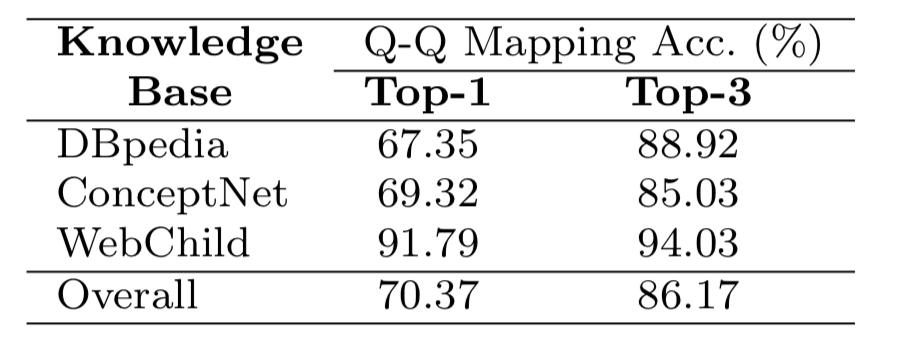
\includegraphics[width=0.5\textwidth]{qqmaping.png}
	\caption{问题到查询映射模型(QQmaping)在测试集中对应的三个知识库的正确率/测试集的分布情况}
	\label{qqmaping}
\end{figure}
引入支持向量机(SVM)\citing{chang2011libsvm}和使用长短期记忆(LSTM)的联合嵌入模型\citing{wu2016value}作为基线模型:只提供问题的SVM-Question和LSTM-Question、只提供图片的SVM-Image和LSTM-Image以及同时提供问题文本和图片的SVM-Question+Image和LSTM-Question+Image,各模型使用FVQA数据集作为训练和测试集中测试,不同模型的正确率见表\ref{fvqa_table}。
% Please add the following required packages to your document preamble:
% \usepackage{multirow}
% \usepackage[table,xcdraw]{xcolor}
% \usepackage{booktabs}
% If you use beamer only pass "xcolor=table" option, i.e. \documentclass[xcolor=table]{beamer}
\begin{table}[H]
% \resizebox{0.5\textwidth}{!}{}
\caption{不同模型在FVQA数据集上的测试正确率,Top-1表示只取得分最高的预测结果,Top-3和Top-10以此类推。灰色数据表示使用与问题对应的完全正确的查询类型时的正确率。}
\begin{tabular}{lccc}
\toprule
\multicolumn{1}{c}{} & \multicolumn{3}{c}{Overall Acc. (\%)}\\
\cmidrule(r){2-4}
\multicolumn{1}{c}{\multirow{-2}{*}{\textbf{Method}}} & \textbf{Top-1}& \textbf{Top-3} & \textbf{Top-10} \\
\midrule
SVM-Qusetion        & 11.19 & 20.68 & 32.14 \\
SVM-Image           & 17.55 & 30.75 & 49.02 \\
SVM-Qusetion+Image  & 17.99 & 31.83 & 49.55 \\
LSTM-Question       & 10.30 & 18.26 & 31.02 \\
LSTM-Image          & 22.69 & 36.21 & 58.59 \\
LSTM-Question+Image & 23.37 & 37.02 & 52.51 \\
\midrule
\cellcolor[HTML]{C0C0C0}gt-QQmaping & \cellcolor[HTML]{C0C0C0}64.23 & \cellcolor[HTML]{C0C0C0}71.58 & \cellcolor[HTML]{C0C0C0}72.74 \\
top-1-gt-QQmaping & 53.63 & 60.70 & 61.59 \\ 
top-3-gt-QQmaping & \textbf{58.19} & \textbf{65.89} & \textbf{66.83} \\
\bottomrule
\end{tabular}
\label{fvqa_table} 
\end{table}

从表\ref{fvqa_table}中Top-1一列可以看出,无论是SVM-Question+Image与SVM-Image之间的正确率差距还是LSTM-Question+Image与LSTM-Image的正确率差值都非常小,这说明问题的解析对于SVM和LSTM这两种模型正确率的提升没有太大的帮助,而两个模型总体的正确率也处于较低的水平,说明统计方法在样本较小的语料库中很难学习到知识间真正的逻辑关联。而FVQA模型使用问题到查询映射模型能从问题文本中提取到关键信息,并能利用关键信息组成有意义的语言结构,再结合额外知识库搜索到正确答案,答案获得的过程反映了推理的过程。gt-QQmaping(灰色背景)使用问题对应的正确查询类型,因此正确率反映了理想状况下FVQA模型从查询类型到生成查询语句过程中的误差情况,知识库查询过程的错误率在30\%左右。top-1-gt-QQmaping与gt-QQmaping之间的差距则代表问题到查询类型70.37\%(见图\ref{qqmaping})的正确率在最终答案的影响,top-3-gt-QQmaping的准确率高于top-1-gt-QQmaping的原因在是因为前者拥有更高的问题到查询类型映射的准确率。

表\ref{fvqa_answerSource}提供了不同方法在不同答案来源上的正确率,对比表中Image和KB两列容易看出,答案来源于视觉概念的准确率在所有模型上均远高于知识库来源,这说明表中涉及的三种模型都只能从图像和问题文本中包含的概念中提取答案,一旦答案涉及都额外知识库中的“新”概念,准确率便急剧下降,即使是使用额外知识库的gt-QQmaping。
\begin{table}[H]
% \resizebox{0.8\textwidth}{!}{}
\centering
\caption{不同方法在不同答案来源上的正确率}
\begin{tabular}{lcccccc}
\toprule
\multicolumn{1}{c}{\multirow{3}{*}{\textbf{Method}}} & \multicolumn{6}{c}{Answer-Source}\\
\cmidrule(r){2-7}
 & \multicolumn{3}{c}{\textbf{Image}} & \multicolumn{3}{c}{\textbf{KB}}\\
\cmidrule(r){2-4}
\cmidrule(r){5-7}
 & \textbf{Top-1} & \textbf{Top-3} & \textbf{Top-10} & \textbf{Top-1} & \textbf{Top-3} & \textbf{Top-10} \\
 \midrule
SVM-Qusetion        & 12.80 & 24.53 & 36.48 & 0.68 & 2.03 & 3.72 \\
SVM-Image           & 19.92 & 34.88 & 55.11 & 2.03 & 3.72 & 9.12 \\
SVM-Qusetion+Image  & 20.43 & 36.07 & 55.73 & 2.03 & 4.05 & 9.12 \\
LSTM-Question       & 11.71 & 20.49 & 34.21 & 1.01 & 3.72 & 10.14 \\
LSTM-Image          & 25.49 & 40.40 & 65.12 & 4.39 & 8.78 & 15.88 \\
LSTM-Question+Image & 26.01 & 41.12 & 58.05 & 6.08 & 10.14 & 16.22 \\
\midrule
\cellcolor[HTML]{C0C0C0}gt-QQmaping & \cellcolor[HTML]{C0C0C0}72.65 & \cellcolor[HTML]{C0C0C0}80.13 & \cellcolor[HTML]{C0C0C0}80.13  & \cellcolor[HTML]{C0C0C0}9.12 & \cellcolor[HTML]{C0C0C0}15.54 & \cellcolor[HTML]{C0C0C0}24.32 \\
top-1-gt-QQmaping & 60.89 & 68.27 & 68.27 & 6.08 & 11.15 & 17.91 \\ 
top-3-gt-QQmaping & \textbf{66.10} & \textbf{74.15} & \textbf{74.15} & \textbf{6.42} & \textbf{11.82} & \textbf{18.92} \\
\bottomrule
\end{tabular}
\label{fvqa_answerSource}
\end{table}

FVQA模型提出了一种以句法结构中的谓语为核心的先验知识问题的解答思路,首先从问题中解析出关键的谓语信息,在问题到查询类型模型中,结合谓语、视觉概念和答案来源决定了28种不同的查询类型,再使用生成的查询语句搜索基于12种谓语构建的知识库,最终预测答案。“主语-谓语-宾语”的一般句式结构中谓语表示了主语和宾语之间的相互作用,即使在相同的主语和宾语情况下,不同的谓语能表达出截然不同的语义信息,而绝大多数问题也能够直接通过谓语,推断答案的范畴。以谓语为基础的优势有几点,第一,易于问题分类。问题的自然语言表达方式众多,但无论如何改变句式结构,表达相同含义的谓语有限,通过对谓语的语义划分能够划分出问题的不同类型。第二,便于知识库的查询。知识库中的实体之间通过不同的谓语连接,形成错综复杂的知识网络,一个实体有众多连接,但一个谓语只连接两个实体,且往往谓语的两端就是问题的答案。

FVQA模型的缺陷有三点,第一,分类数量的确定和分类模型的精度。FVQA模型由于查询语句的生成依赖于查询类型,因此问题到查询类型映射的准确性会直接影响到答案生成的正确率。表\ref{fvqa_table}是在FVQA数据集上进行的,由于数据集中问题的类型只有28种,因此FVQA模型在问题到查询类型映射模型中使用了28类的分类器,但在实际问答环境中问题类型的具体数量远远多于28种,且无法预先确定,想训练能应用于实际情景中的FVQA模型不仅需要数据集的扩充,还需要提高模型本身的分类精度。第二,不能回答以谓语为答案的问题。所有28种查询类型都要求能从问题中提取关键谓语,并且所有答案都是物体对象,如果问题询问对象之间的关系,模型则无法从问题文本中获得谓语,不能得到答案。第三,不能很好的处理含有多个动词的复杂推理问题。FVQA模型的查询语句过于简单,仅仅将一次查询结果作为答案,在面对需要多级推理的问题时,便无法直接得到答案,如表\ref{fvqa_wrong}。
\begin{table}[H]
% \resizebox{0.8\textwidth}{!}{}
\centering
\begin{tabular}{lcccccc}
\toprule
\multicolumn{2}{c}{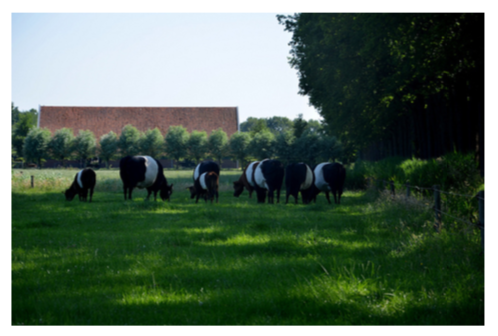
\includegraphics{cow.png}} \\
\multicolumn{2}{c}{What is related to the animal that can be found in this place?} \\
\midrule
\multirow{2}{*}{Mined Facet:} & You are likely to find a cow in a picture \\
 & The cow is related to the tree \\
Predicted Answer: & cow \\
Ground Truth: & tree \\
\bottomrule
\end{tabular}
\caption{问题中包含related和found两个动词,FVQA模型只能提取一个作为谓语并查询,选择found为谓语时,会出现错误的预测}
\label{fvqa_wrong}
\end{table}

\textbf{基于知识库的通用嵌入模型}
无论是Ahab还是FVQA模型都是通过将问题固定在一定类型,再通过对应不同问题的类型的额外知识库查询,获得更丰富的知识,从而提高复杂问题的正确率。为了提高视觉问答系统的问题的灵活性,Wu等人又通过改进常见的CNN+LSTM的嵌入模型,提出了基于知识库的通用嵌入模型。模型的基本架构由图像属性提取网络(CNN)、图像描述生成网络、外部知识库查询网络以及答案生成网络(LSTM)构成,模型架构如图\ref{KBLSTM}。
\begin{figure}[H]
	\centering
	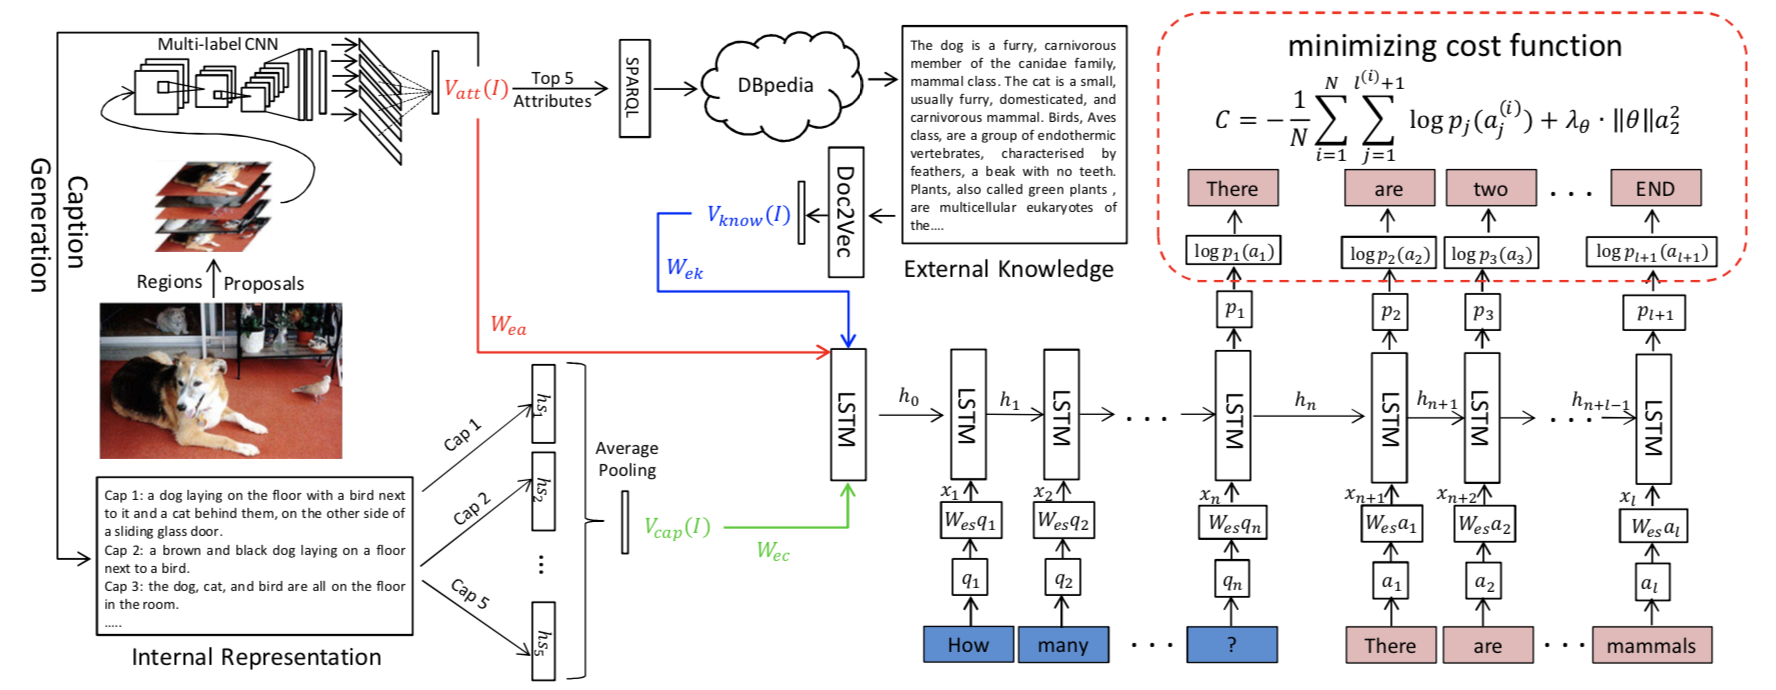
\includegraphics[width=0.8\textwidth]{KBLSTM.png}
	\caption{结合外部知识库的通用嵌入模型}
	\label{KBLSTM}
\end{figure}

图像属性提取网络将图像属性提取问题视为多标签的分类问题,以图像的多个子区域作为输入,输出前五个从MS COCO中筛选得到的图像属性$V_{att}(I)$,属性可能为物体名称、动作或者描述特征的形容词。提取出的图像属性分别作为图像描述生成网络和外部知识库查询网络的输入,图像描述生成网络将\cite{wu2016value}中的高层次的属性表达输入LSTM网络生成基于图像属性的描述,再将文本描述转化为五个特征向量,平均池化所有向量得到向量$V_{cap}(I)$。外部知识库查询网络首先分别将五个图像属性转化为知识库查询语言,查询到DBpedia知识库中相应的对象后,返回其“comment”——“comment”往往包含关于知识库对象最重要的解释信息,如图\ref{SPAQLexample},为了将大段的“comment”转化为向量,Wu等人使用Doc2Vec\citing{le2014distributed}——一种能方便的将句子、段落甚至文章等不固定长度的文本转化为固定大小的向量的模型,并且能包含文本内容的语义信息。——将其转化为$V_{know}(I)$。最后将$V_{att}(I)$、$V_{cap}(I)$、$V_{know}(I)$以及问题文本作为答案生成网络(LSTM)的输入,训练网络生成答案。
\begin{figure}[H]
	\centering
	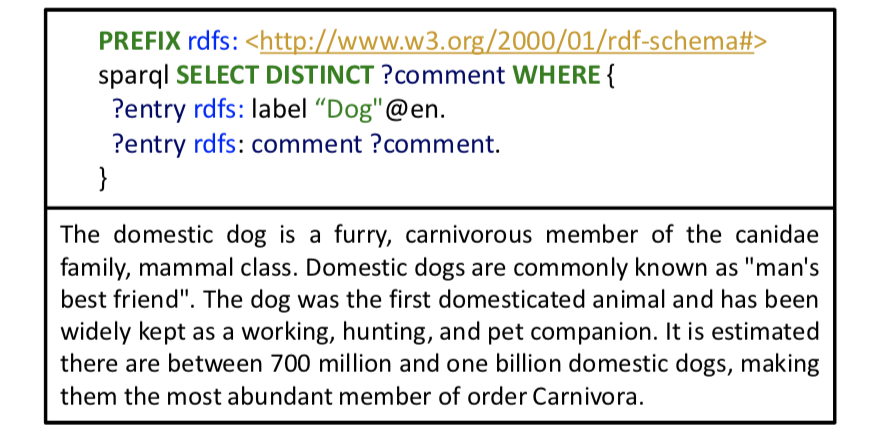
\includegraphics[width=0.5\textwidth]{SPAQLexample.png}
	\caption{使用‘dog’属性的查询语句以及返回的‘comment’内容}
	\label{SPAQLexample}
\end{figure}

在评估模型准确率时,由于该模型面对开放性问题,因此不同于Ahab和FVQA只能使用专门设计的数据集,该模型采用Toronto COCO-QA\citing{ren2015exploring}和VQA\citing{antol2015vqa}两个数据集进行评测。为了说明该模型的正确率情况,引入基线模型和几个结果较优的模型正确率作为对比,GUESS表示随机猜测模型,VggNet-LSTM使用在ImageNet上预处理的VggNet网络连接LSTM得到,VggNet+ft-LSTM使用在图像属性分类任务上微调后的VggNet,Att-LSTM表示直接将$V_{att}$作为LSTM输入的变体模型,类似的变体有Att+Cap-LSTM、Att+Know-LSTM、Att+Cap-LSTM、Cap+Know-LSTM,以及完整的Att+Cap+Know-LSTM模型。不同模型在两个数据集的正确率分别如表\ref{Wucoco}和\ref{Wuvqa}。
\begin{table}[H]
% \resizebox{0.8\textwidth}{!}{}
\centering
\caption{不同模型在Toronto COCO-QA正确率的表现}
\begin{tabular}{lc}
\toprule
\textbf{Toronto COCO-QA} & Acc(\%)\\
\midrule
GUESS\citing{ren2015image} & 6.65 \\
VggNet-LSTM & 50.73 \\
VggNet+ft-LSTM & 58.34 \\
\midrule
Att-LSTM & 61.38 \\
Att+Cap-LSTM & 69.02 \\
Att+Know-LSTM & 63.07 \\
Cap+Know-LSTM & 64.31 \\
\midrule
Att+Cap+Know-LS & \textbf{69.73} \\
\bottomrule
\end{tabular}
\label{Wucoco}
\end{table}

\begin{table}[H]
% \resizebox{0.8\textwidth}{!}{}
\centering
\caption{不同模型在VQA数据集的正确率表现}
\begin{tabular}{lc}
\toprule
\textbf{VQA} & Acc(\%)\\
\midrule
VggNet-LSTM & 44.93 \\
\midrule
Att-LSTM & 51.60 \\
Att+Cap-LSTM & 55.04 \\
Att+Know-LSTM & 53.79 \\
Cap+Know-LSTM & 52.31 \\
\midrule
Att+Cap+Know-LS & \textbf{55.96} \\
\bottomrule
\end{tabular}
\label{Wuvqa}
\end{table}

\section{本文的主要贡献与创新}
正如以上提到的诸多模型的探索,视觉问答领域正在迎来百花齐放的局面。模型的多样性和答案的准确率会同时受惠于目前机器学习在计算机视觉、自然语言处理和知识表达与推理的成功应用。然而,除了颇具前景的应用方向和深远的研究意义,视觉问答仍然属于起步阶段,面临着诸多亟待解决的问题。

第一,泛化能力受限于数据集。目前的视觉问答主流模型为联合嵌入模型,其主要思路为联合图像处理模型输出的图像特征和自然语言处理输出的文本特征,并利用神经网络训练联合后的特征,得到答案。和其他基于神经网络的模型一样,联合嵌入模型的泛化性能主要由训练集的大小、多样性等因素影响,然而数据集的收集和整理工作需要大量的人工成本。因此“数据集偏见”成为目前模型泛化性能的主要瓶颈之一。

第二,结果的可解释性匮乏。目前的视觉问答模型大多仍然属于分类模型,候选答案来源于训练集,模型对候选答案评分,并将得分最高的候选答案作为输出。而分类的标准存在于模型中的大量参数之中,模型得出答案的过程和标准并不明确。匮乏的可解释性在需要多步推理的问题上表现尤为突出。该类问题不同于识别任务,答案的得出是分步进行的,每一步的正确推理都对答案的得出至关重要。而通过分类模型得出的答案无法给出每一步的推理过程。

第三,缺少通用架构。除了以上提到的联合嵌入模型,另一个重要的研究方式是基于知识库的视觉问答模型。基于知识库的视觉问答模型的提出便是为了解决训练集的有限性和答案的黑盒性。外源知识库能够扩展模型可搜寻的答案范围,结构化且语义明确的实体之间的关系也可以提供答案的可解释性。然而,目前基于知识库的视觉问答模型根据各自的特点建立独特的数据集,该类自建的数据集从数据量和多样性的角度相较于更为通用的数据集,例如VQA2.0\citing{goyal2017making},都更差。并且由于使用的数据集不同,模型之间很难在统一地衡量各自的性能,造成了联合嵌入模型和基于知识库的VQA模型的割裂。

为解决以上提到的所有问题,本文将提出一种通用的视觉问答架构——Compound VQA(CPVQA)模型。CPVQA模型的提出基于以下假设:所有视觉问答任务可以根据问题划分为两个类别,回答第一类问题需要外源知识或者常识,即KB-specific类,另一类问题的答案可以直接从问题和图像中得到。例如,对于图\ref{DogExample},问题1:“图片中的狗是什么颜色?”,模型可以通过直接识别出图像中狗的色彩属性得出正确答案,而对于问题2:“图片中的动物是什么颜色?”,模型除了需要正确识别图片中的狗和颜色属性,还需要知道“狗属于动物”的常识,才能在“狗的颜色”——黄色和“草地的颜色”——绿色之间做出正确的预测。

\begin{figure}[H]
	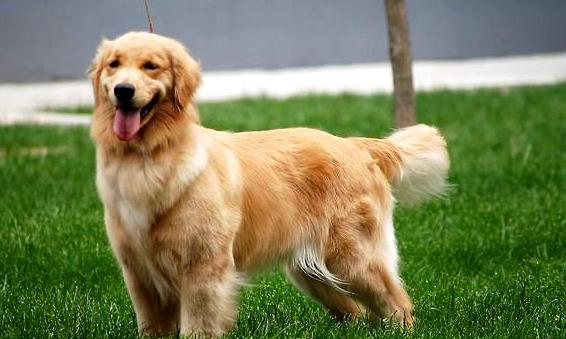
\includegraphics[width=0.8\textwidth]{DogExample.jpg}
	\caption{对于同一张图片,问题的不同将会决定模型是否需要外源知识或是常识。}
	\label{DogExample}
\end{figure}

基于以上的假设,本文从数据集增强、模型架构等方面进行了研究,以下为主要贡献和创新点。

1. 构建增强的数据集Classified VQA2.0(CVQA)。CVQA数据集以VQA2.0为基础,依照问题是否涉及外源知识或常识为标准,对原有数据添加“KB-specific”维度,将问题分为KB-specific(KBS)和none KB-specific(N-KBS)两类。

2. 提出一种通用的视觉问答架构——Compound VQA模型。本文提出的Compound VQA模型由KB-Specific Network(KBSN)和None KB-Specific Network(N-KBSN)两个模型组成。KBSN由实体与属性识别模型构成的前置模块(pre-KB module)和知识库(KB module)组成,用于处理KBS的问题。N-KBSN处理“N-KBS类的问题。

3. N-KBSN使用联合嵌入模型的思路,由Faster R-CNN\citing{ren2015faster}得到图像特征,由ELMo模型\citing{Peters:2018}训练得到文本特征,并引入注意力机制——MCA\citing{Yu_2019_CVPR}训练得出答案。

4. KBSN共用N-KBSN中的特征表示,从图像和问题中抽取实体和属性信息,使用SPARQL转化为知识库查询语句,最终从知识库中得到答案。

\section{本论文的结构安排}
本文的章节结构安排如下:

\chapter{视觉问答任务及基础架构}
虽然视觉问答任务是从2014年才被提出的新兴人工智能领域,但是由于其跨学科的特性以及图像处理和自然语言处理领域的快速发展,目前视觉问答模型迭代速度也非常快,大量的数据集、模型被提出。本章将介绍视觉问答研究中重要的基础知识和模型的基础架构。

\section{视觉问答任务}
视觉问答是向智能系统给出图片和问题,系统返回答案的任务。由于图像内容的复杂性和问题的开放性,视觉问答的研究难度较大,正因如此,其相较于其他子任务更接近通用人工智能。本节我们将详细分析其问题类型,并介绍目前主要的数据集。
\subsection{问题类型划分}
由于视觉问答任务的最终目的是面向真实的人类交互场景,因此VQA模型需要解决开放性问题的挑战,问题类型的研究是构建模型前的关键步骤之一。

按照问题的形式划分,视觉问答的问题可以分为二值否问题\citing{krishna2017visual,zhu2016visual7w,andreas2015deep}、多选问题\citing{antol2015vqa,zhu2016visual7w}、开放性问题\citing{antol2015vqa}。按照问题的内容划分,问题分为识别类和推理类。识别类问题包括物体识别、物体检测、属性分类、计数问题、空间关系判定,此类任务在以往的计算机视觉的研究中已经达到了较高的识别准确率,在某些物体识别和物体检测任务上已经能迫近甚至超越人类水平。推理类问题包括场景识别、常识推理和知识库推理等,这类问题形式多变、层次复杂、需要外源知识、甚至需要多步推理,例如:“图片中有什么东西在伞下?”——需要能准确识别物体的空间位置关系、“图片中的交通路口是否可以通行?”——需要基于常识的推理、“图片中的汽车属于什么品牌?”——需要基于外部专业知识库提供隐藏信息。

除了以上提到的两种问题分类,本文提出了一种全新问题分类标准——按照答案与问题和图像的相关性划分。我们认为:对于不同的视觉问答问题,其答案-图像相关度、答案-文本相关度存在差异,即有的答案更依赖于准确的图像分析,而有的答案却对图像不敏感。而这种与输入信息的相关性差异能帮助我们更好的理解模型决策的内部机制。我们提出以Q、q、I、i定性的表示“答案-问题强相关”、“答案-问题弱相关”、“答案-图像强相关”、“答案-图像弱相关”,从而组合得出四种问题类型QI、Qi、qI、qi,如表\ref{ques_type}所示。
\begin{table}[H]
% \resizebox{0.8\textwidth}{!}{}
\centering
\caption{根据答案和源信息的相关性划分出四类任务}
\begin{tabular*}{0.9\textwidth}{@{\extracolsep{\fill}}lccc}
\toprule
& \textbf{答案-问题相关性} & \textbf{答案-图像相关性} & \textbf{问题类型} \\
\midrule
\multirow{4}{*}{\textbf{相关性}} &  强& 强&  QI\\
&  强& 弱&  Qi\\
&  弱& 强&  qI\\
&  弱& 弱&  qi\\
\bottomrule
\end{tabular*}
\label{ques_type}
\end{table}

QI类型的问题需要同时结合图像特征和文本特征,这是一种最典型的视觉问答类型。Qi类型的问题答案可以直接根据问题文本得出,这类图像无关的问题可以退化为文本问答任务。qI类型的答案可以直接从图像中得出,这类问题退化为图像识别任务。例如,对于图\ref{DogExample},问题1:“图片中的狗是什么颜色?”,模型可以通过直接识别出图像中狗的色彩属性得出正确答案,那么问题1就是qI类型。对于同样的图片,问题2:“图片上的狗是不是属于动物?”是图像无关的Qi类型。
\begin{figure}[H]
	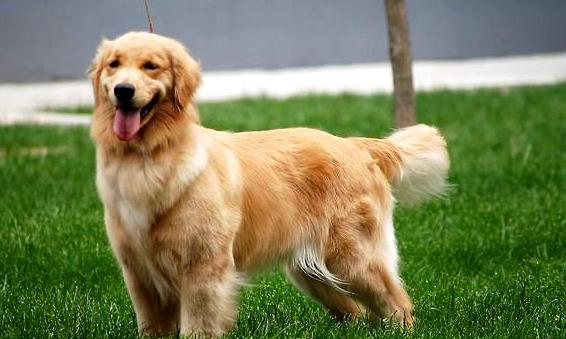
\includegraphics[width=0.8\textwidth]{DogExample.jpg}
	\caption{视觉问答示例图}
	\label{DogExample}
\end{figure}

qi类型的问题答案与问题文本和图像的相关性都比较弱,这类问题包含两类类型,一类为错误或者偏僻的问题,例如偏僻单词的问题、低频的语法结构;另一类为涉及常识和外源知识的问题,回答这类问题需要额外的知识,甚至还需要多步的推理,例如,对于图\ref{DogExample},问题3:“图片中的动物是什么颜色?”,模型除了需要正确识别图片中的狗和颜色属性,还需要知道“狗属于动物”的常识,才能在“狗的颜色”——黄色和“草地的颜色”——绿色之间做出正确的预测。目前,对于错误或者偏僻的qi问题研究较少。

\subsection{视觉问答数据集}
视觉问答任务是在经历了计算机视觉和自然语言处理任务成功之后,新兴出现的人工智能任务——要求系统能同时理解多模信息,并完成信息整合与推理。自从2014年以来,多个高质量的视觉问答数据集被提出:DAQUAR\citing{malinowski2014multi}、COCO-QA\citing{ren2015exploring}、VQA\citing{antol2015vqa}、VQA 2.0\citing{goyal2017making}、CLEVR\citing{johnson2017clevr}、KB-VQA\citing{wang2015explicit}、FVQA\citing{wang2017fvqa}。

以上的数据集有不同的图像来源,各自的问题对的数量也不同,但是其中最重要的区别在于问题回答是否需要额外知识,例如常识和专业知识。我们将不需要额外知识的数据集称为“基于视觉的数据集”——问题的答案往往来源于图像信息的准确提取,而需要额外知识的数据集称为“基于知识的数据集”——图像信息仅仅作为推理的一环,答案依赖于图像和问题以外的知识。根据以上的划分标准,以上提到的数据集的统计信息如表\ref{dataset_compar}。正如表格所示,KB-VQA和FVQA属于“基于知识的数据集”,其他均属于“基于视觉的数据集”。
\begin{table}[H]
% \resizebox{0.8\textwidth}{!}{}
\centering
\caption{视觉问答数据集的对比}
\begin{tabular*}{0.9\textwidth}{lrrcc}
\toprule
\textbf{Dataset} & \textbf{\#images} & \textbf{\#QA pairs} & \textbf{Image source} & \textbf{Knowledge based}\\
\midrule
DAQUAR\citing{malinowski2014multi}&  1,449& 12,468&  NYU-Depth& \\
COCO-QA\citing{ren2015exploring}&  69,172& 117,684&  COCO& \\
VQA\citing{antol2015vqa}&  204,721& 614,163&  COCO& \\
VQA 2.0\citing{goyal2017making}&  204,721& 1,105,904&  COCO& \\
CLEVR\citing{johnson2017clevr}&  100,000& 999,968&  Synthetic images& \\
\midrule
KB-VQA\citing{wang2015explicit}&  700& 2402&  COCO+ImgNet& $\surd$\\
FVQA\citing{wang2017fvqa}&  1,906& 4,608&  COCO& $\surd$\\
\bottomrule
\end{tabular*}
\label{dataset_compar}
\end{table}

\subsubsection{基于视觉的数据集}
\textbf{DAQUAR}\qquad
DAQUAR从NYU-Depth V2中带有语义分割标注的图片基础上扩展而来\citing{malinowski2014multi}。数据集包含1449张图片,图片多为室内场景,这大大地限制了数据集的场景丰富性,是该数据集的一大劣势。数据集由训练集和测试集两部分组成,训练集中包含6794对“问题-答案”,测试集中包含5674对“问题-答案”,“问题-答案”对由算法生成或是人类志愿者提供,算法生成的“问题-答案”对根据给定的模板生成。
% \begin{figure}[H]
% 	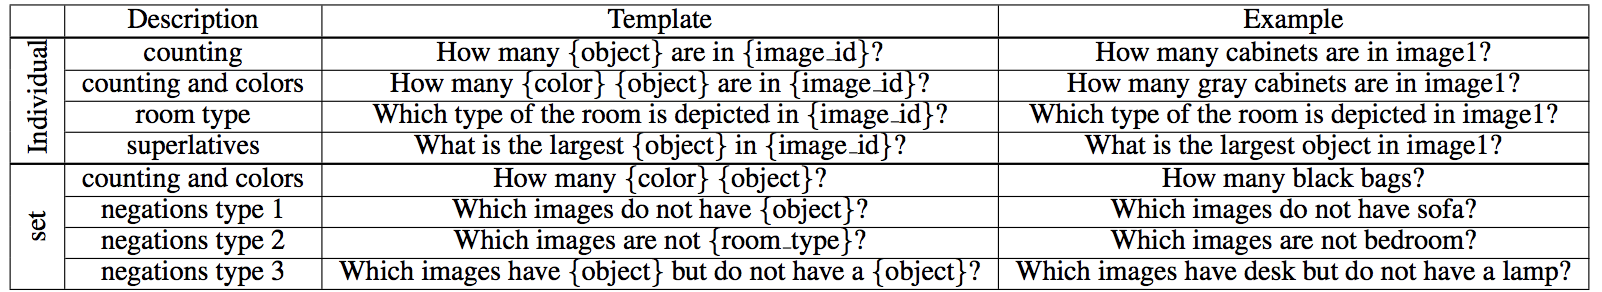
\includegraphics[width=0.8\textwidth]{DAQUAR.png}
% 	\caption{DAQUAR问题模板}
% 	\label{DAQUAR}
% \end{figure}

% DAQUAR数据集较小并且问题的类型只有三种:物体识别、色彩识别、计数,并且答案类型多以单词为主,因训练和测试系统复杂问题的推理能力较弱,偏于传统的物体识别任务。

\textbf{COCO-QA}\qquad
COCO-QA包含来自MS COCO的123287张真实场景图片,问题-答案对则是运用算法从MS COCO数据集的图像标注中生成的,为了方便生成算法的运用,将问题划分在物体识别、色彩识别、计数、地点查询四种类型。DAQUAR数据集在实际测试过程中,被发现仅仅通过简单的猜测答案的方式都能获得较高的正确率,这使得高准确率出现了极大的偏差,不能公正的测试系统的“推理”能力。为了克服该缺点,COCO-QA去除了出现频数极低和极高的一些答案,使得常见答案出现的评率从24.98\%下降到7.30\%。COCO-QA的训练集包含78736对“问题-答案”,测试集包含38948对“问题-答案”。
% 在四个类别中的分布如图\ref{coco-vqa}。
% \begin{figure}[H]
% 	\centering
% 	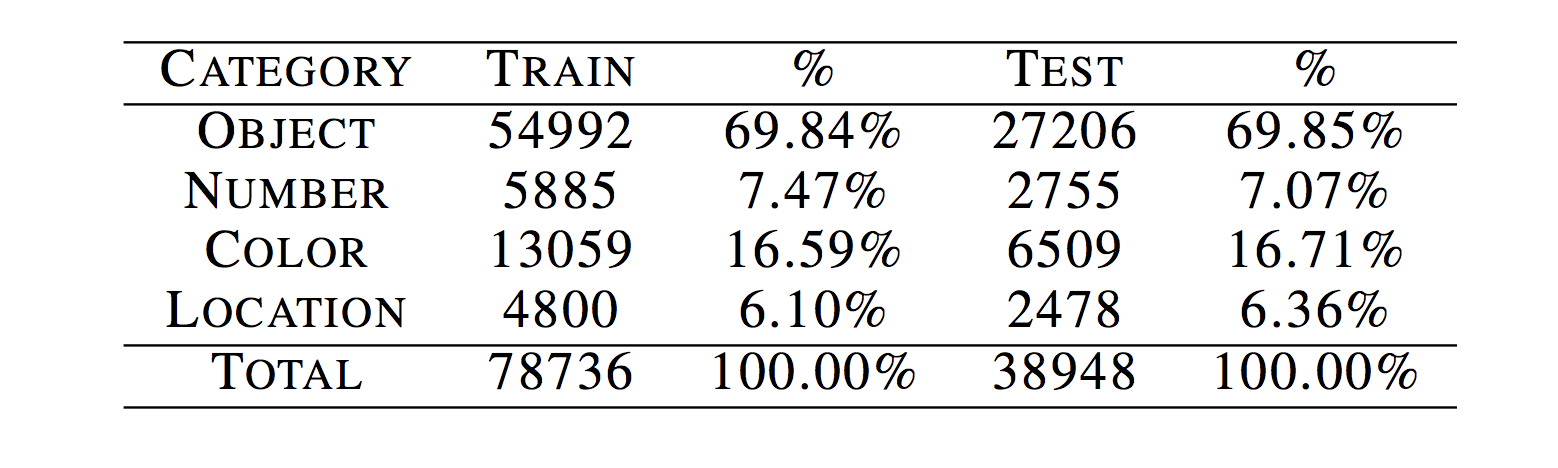
\includegraphics[width=0.8\textwidth]{coco-vqa.png}
% 	\caption{coco-vqa中“问题-答案”对的分布情况}
% 	\label{coco-vqa}
% \end{figure}

\textbf{VQA}\qquad
VQA数据集是视觉问答领域发展的一个重要拐点,在此之前的数据集的问题类型被限制在一些模板之中,这使得数据集不能很好地测试出视觉问答系统在真实语境下的表现,例如,DAQUAR将答案仅仅限制在16种基本颜色和894种物体类别中\citing{malinowski2014multi}。VQA数据集中的问题和答案是无限制、开放式的,且全部由人类产生,同时图片的数量相较DAQUAR提高了两个数量级,到达254731张,极大的提高了数据集的容量。VQA数据集不仅包含从MS COCO\citing{lin2014microsoft}中提取的204721张真实场景的图片,还提供了50000张合成的抽象场景图,丰富了数据库场景的多样性,同时为高阶的场景推理和复杂空间推理提供了便利。
% \begin{figure}[H]
% 	\centering
% 	\subfigure[真实场景图像实例]{
% 		\label{vqa-real}
% 		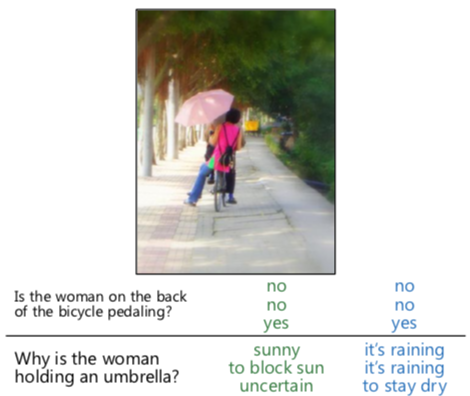
\includegraphics[width=0.4\textwidth]{VQA-real.png}}
% 	\subfigure[抽象场景图像实例]{
% 		\label{vqa-abs}
% 		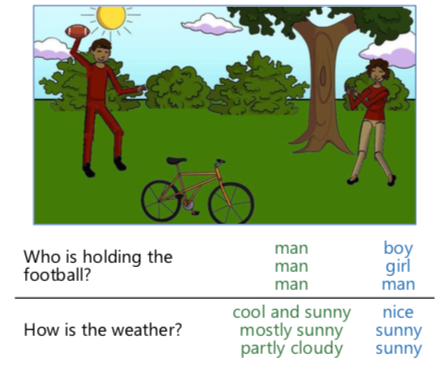
\includegraphics[width=0.4\textwidth]{VQA-abs.png}}
% 	\caption{VQA中的真实、抽象场景图像实例}
% 	\label{vqa-exmaple}
% \end{figure}

% 为了实现对复杂推理的训练和测试,VQA数据集在问题设置上采用了人工的方式,每张图片都有3个人类提出的问题。答案则分为开放式和多项选择两种形式,开放式答案由于答案并不唯一,因此难以确定标准答案,因此正确答案的评估方法也引入人工评估机制:对于同一个开放性问题由十个人分别作答,如果有三个及以上的被测者均提供了同一答案,该答案被视为正确答案。多项选择的答案则由四种类型、18个候选项组成(如图\ref{vqa-multi}):
% \begin{description}[labelindent=2em, leftmargin=6em, style=sameline]  
% \item [正确答案] 一个,从被测者回答中取最为常见的作为正确答案
% \item [混淆答案] 三个,不看图,仅根据问题作答的答案
% \item [常见答案] 十个,数据集中最出现频数最高的十个答案
% \item [随机答案] 四个,除去已经列出的选项,随机挑选四个答案
% \end{description}
% \begin{figure}[H]
% 	\centering
% 	\subfigure[真实场景图像的多选实例]{
% 		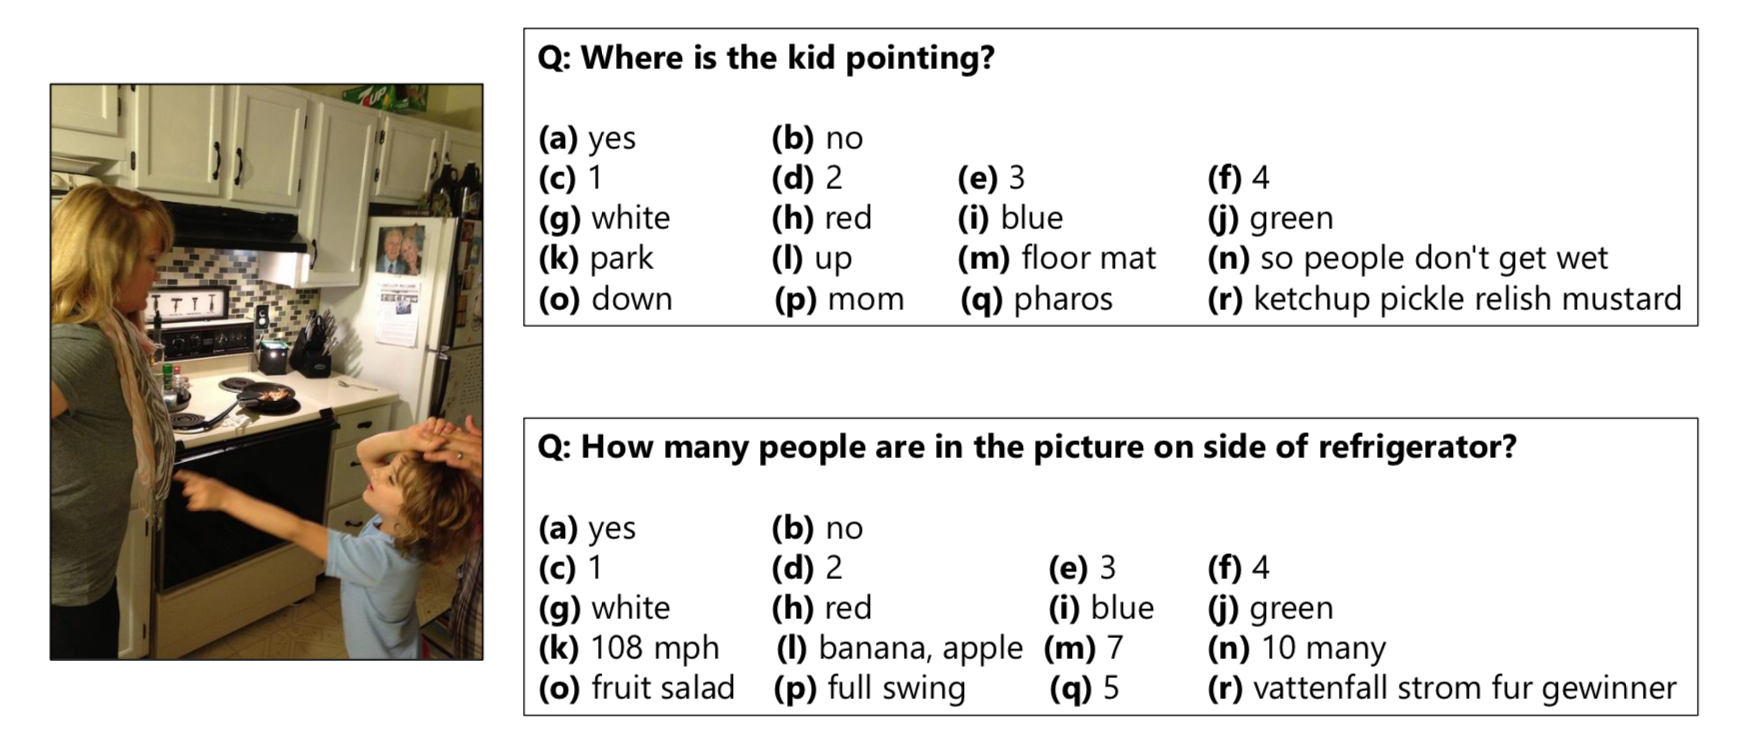
\includegraphics[width=0.8\textwidth]{vqa-multi.png}}
% 	\subfigure[抽象场景图像的多选实例]{
% 		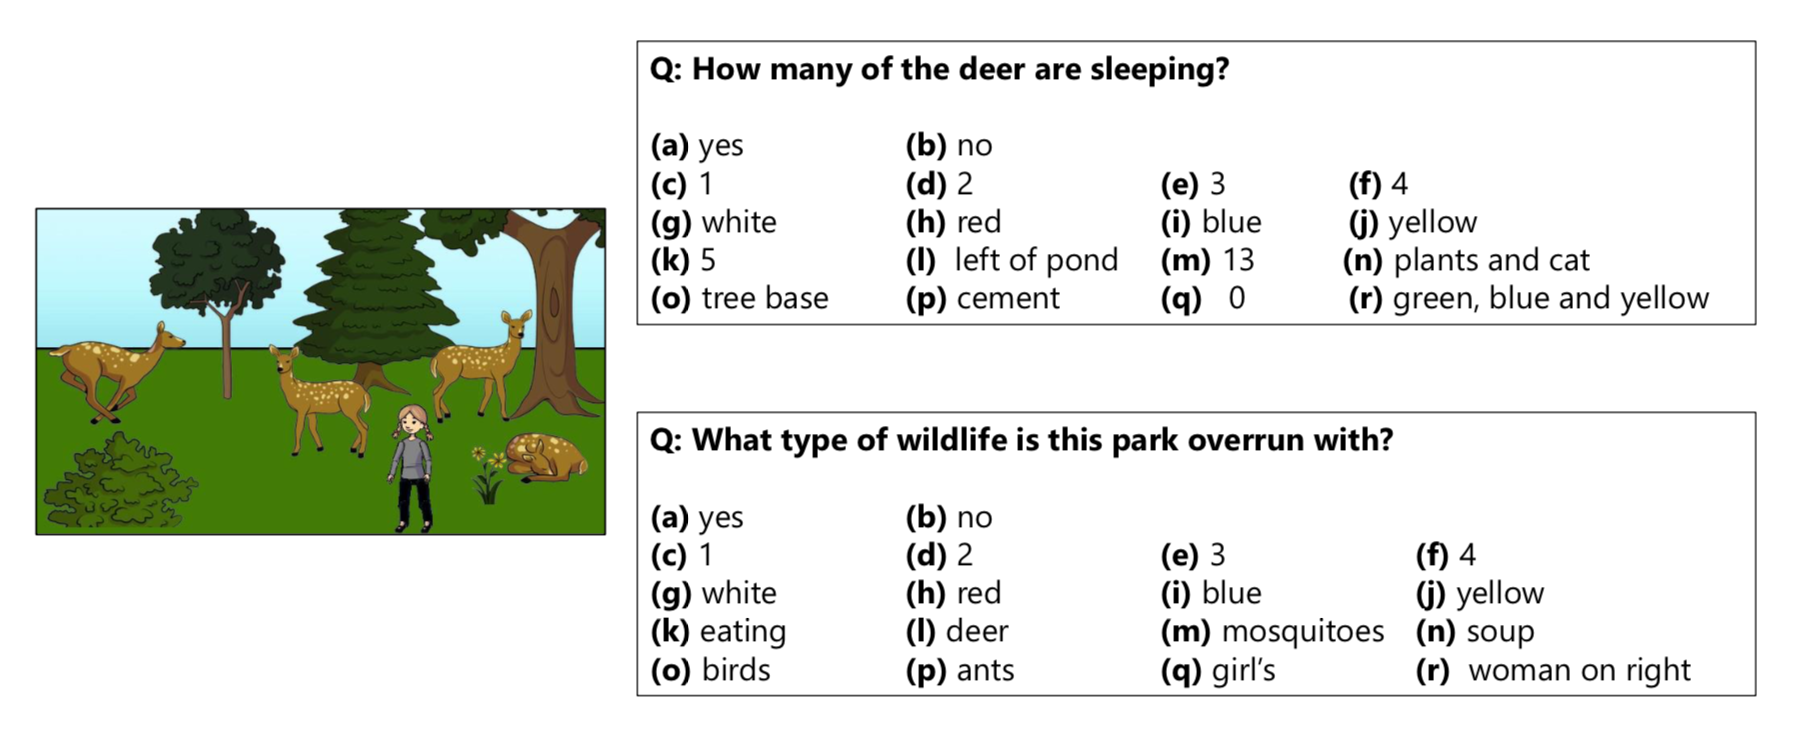
\includegraphics[width=0.8\textwidth]{vqa-multi2.png}}
% 	\caption{VQA中的真实和抽象场景图像的多项选择实例}
% 	\label{vqa-multi}
% \end{figure}


% VQA数据集由于其建立了开放性问题和多项选择问题的评测标准,成为众多算法的测试数据集,但VQA数据集存在语言偏见问题。具体表现为,即使是完全无视图像的算法也能在VQA数据集上得到49.6\%的准确率\citing{ren2015exploring},这意味在VQA数据集的测试环境下,系统对于视觉信息的需求程度远远小于语言信息,这种状况相较于人类对于图像问答任务中的真实体验而言,是严重不符的。例如,答案为”是或否“的问题占所有问题的38\%,并且大约59\%的二值问题答案都为”是“;询问”什么运动“的问题中有41\%的答案为”网球;询问数量的问题中有39\%的答案为“2”。
\textbf{VQA 2.0}\qquad
针对VQA数据集的语言偏见问题,VQA 2.0通过在原有的VQA数据集基础上补充新的“混淆数据”实现数据集对视觉信息的增强。“混淆数据”和原始数据一样由(图像I,问题Q,答案A)的形式组织,不同的是新补充的图像与原有图像相似,但回答同样的问题Q却得到不同的答案A。针对同样的问题,在不同图片背景下需要得到不同的答案,这要求系统不仅能理解自然语言问题,同样需要关注图片的语义差异,才能得到正确的答案,这种平衡的方法能够筛选掉弱化图像理解的算法,强化了图像理解在视觉问答任务的重要性。补充后的VQA 2.0包含110万对”图像-问题“、20万张关联1300百万个问题的真实场景图片,数据量几乎是VQA数据集的两倍,成为了开放性问题的新测试标准。
% \begin{figure}[H]
% 	\centering
% 	\subfigure[]{
% 		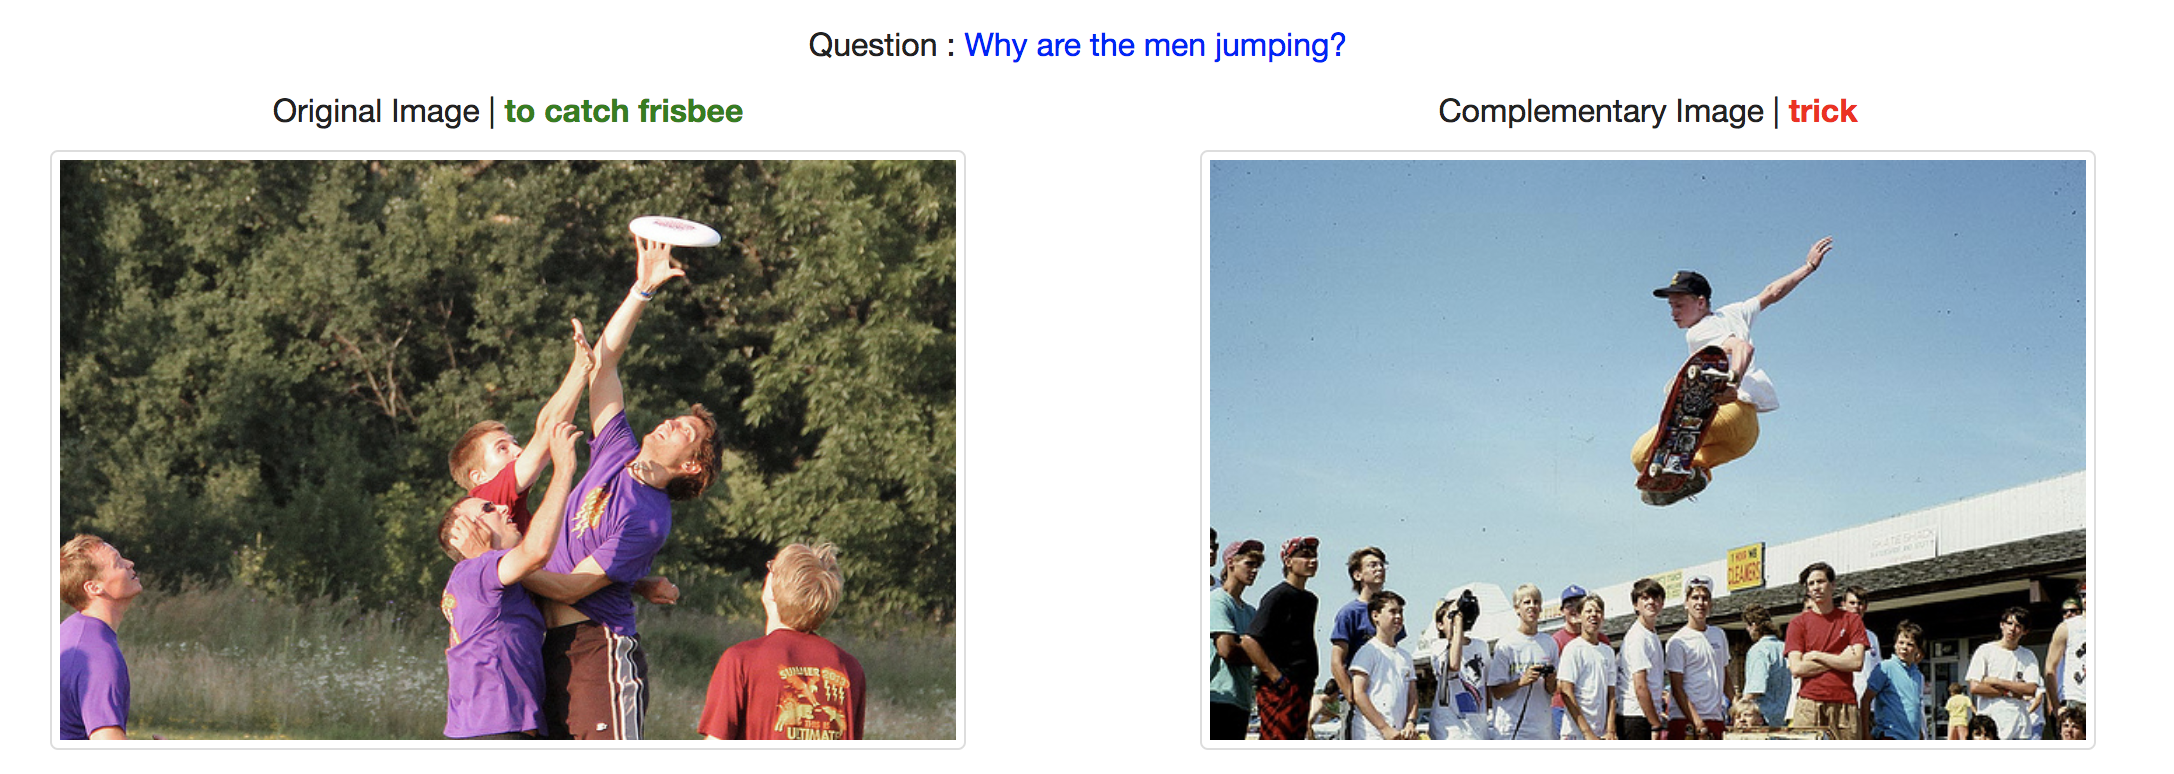
\includegraphics[width=0.8\textwidth]{vqa2-1.png}}
% 	\subfigure[]{
% 		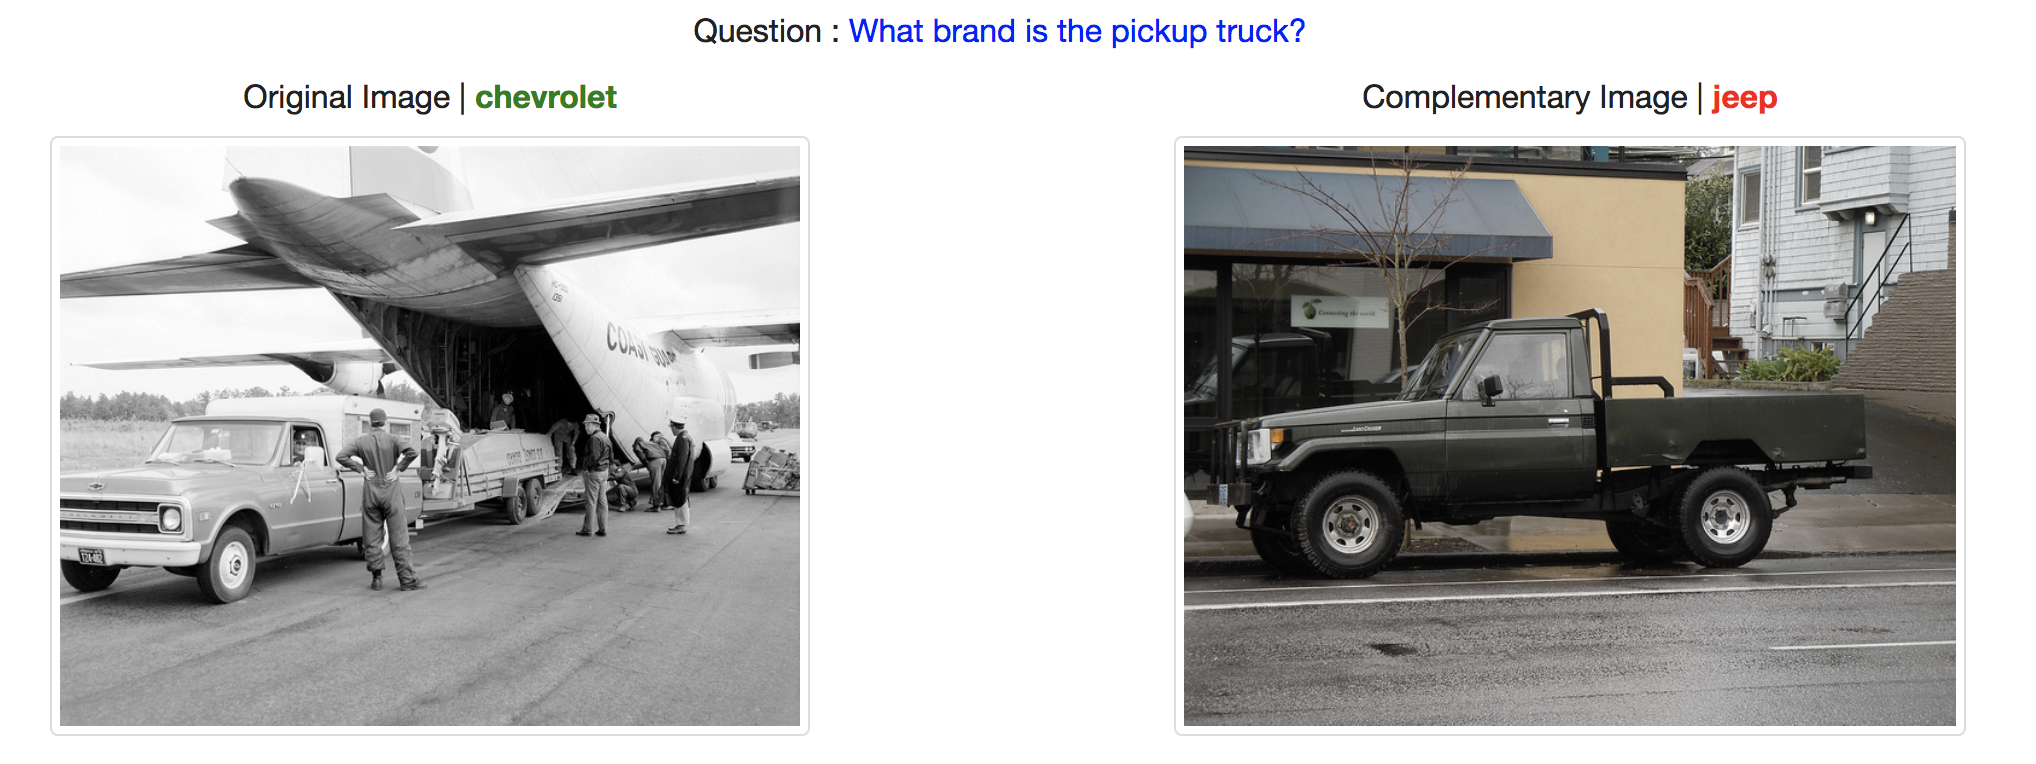
\includegraphics[width=0.8\textwidth]{vqa2-2.png}}
% 	\caption{VQA 2.0中针对同一问题的不同图像和答案实例}
% 	\label{vqa2}
% \end{figure}

\textbf{CLEVR}\qquad
为了更加准确地衡量视觉问答系统各个方面的推理能力,Johnson等人提出了一个结合语言和基本视觉推理诊断数据集CLEVR。CLEVR包含10万张由空间立方体组成的合成图像、将近100万个问题,其中包含85.3万个独特的问题。在图像的设置上,CLEVR为了减小识别难度,关注系统的视觉推理能力,采用了由空间立方体组成的合成图像,并且每张图像均有包含所有物体位置和属性的说明。CLEVR的问题也均由程序生成得到,涉及属性识别、计数、比较、逻辑运算等子任务。

% 为了减少问题的偏见,数据集生成的问题中有85\%是独特的;为了控制问题的准确性,数据集剔除了有歧义的问题,例如,询问“正方体右边的球体是什么颜色?”时,如果“正方体”右边有多个“球体”,问题便产生歧义,答案变得不唯一,使得评估过程变得复杂和不准确;为了保持问题的复杂性,数据集拒绝了一些看似复杂但实际上限定条件无效的问题,例如,询问“球体前面的圆柱体是否为金属的?”时,如果场景中仅有一个“圆柱体”,那么问题中的“球体前面”的限定便可以被忽略,这种情况降低了问题的复杂性。

% 由于CLEVR数据集对图像和问题具有完全的掌控,能实现其他数据集难以实现的能力测试,要求系统具有短期的记忆力、注意力机制、组合推理能力。
% 但同样因为其简单的图像场景设置,CLEVR不能测试出视觉问答系统在常识推理、复杂推理的表现,并且也不能衡量系统在真实场景中的识别能力和稳定性。
% \begin{figure}[H]
% 	\centering
% 	\subfigure[尺寸、形状、样色、材质的标注]{
% 		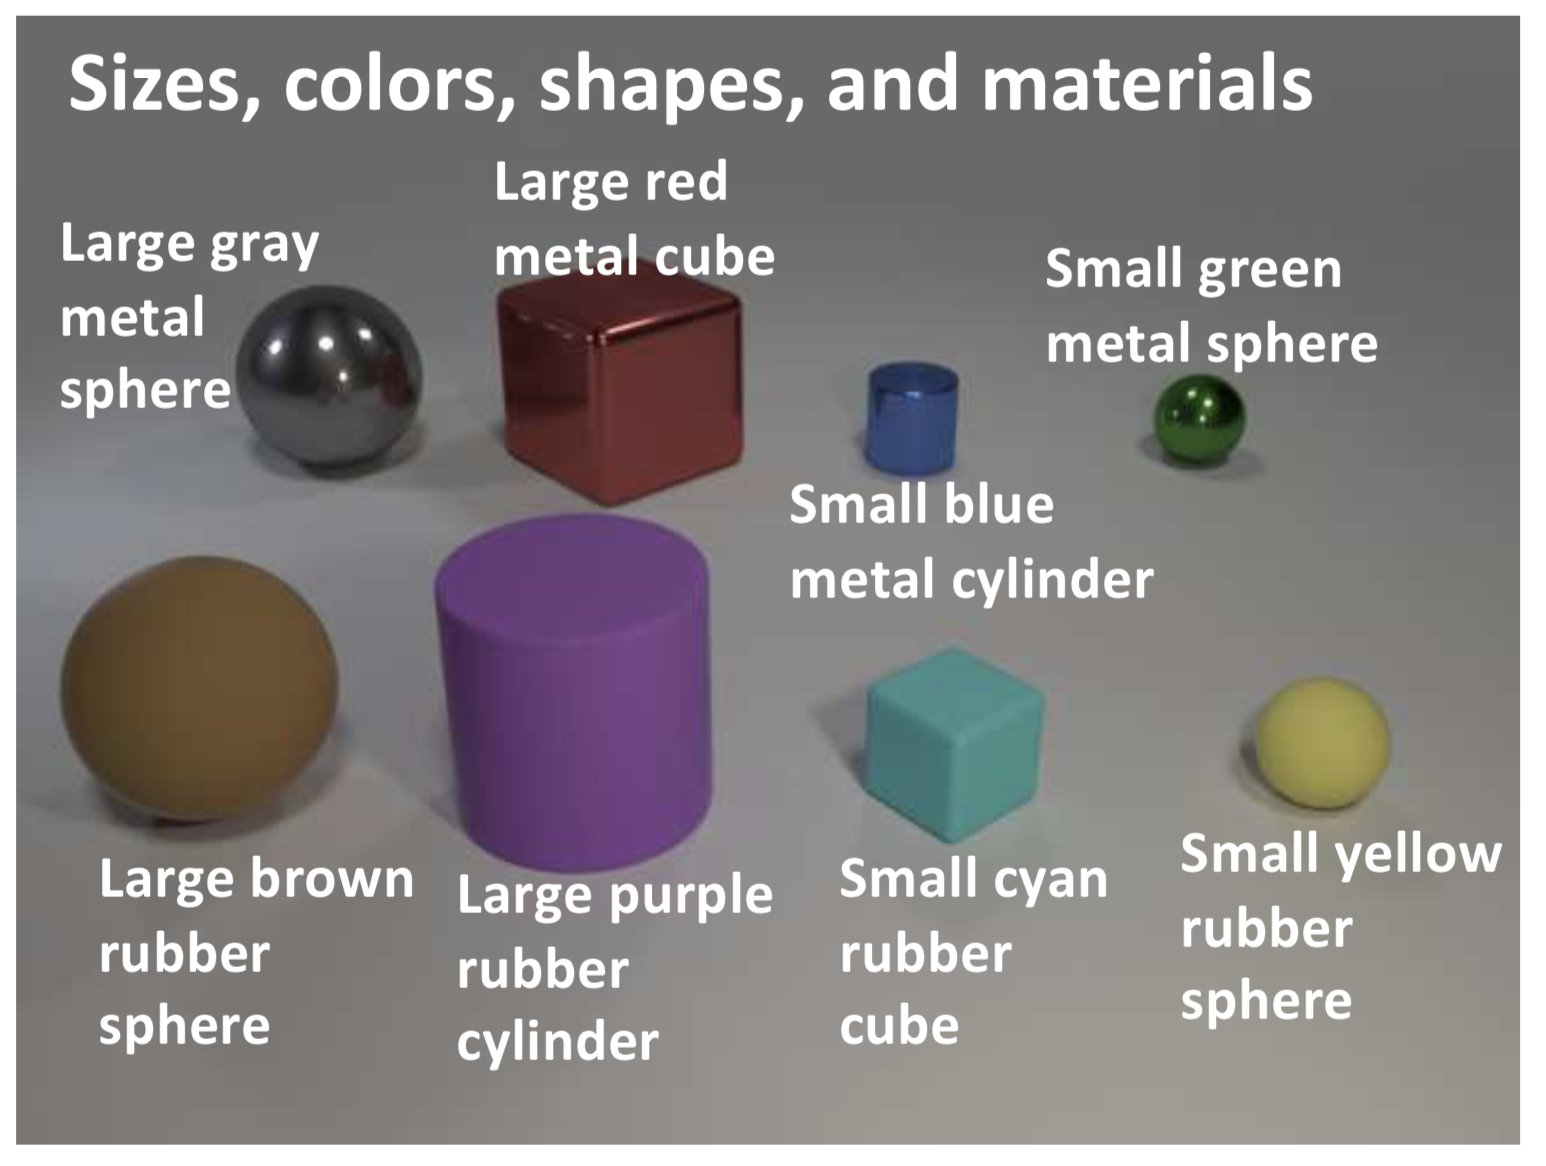
\includegraphics[width=0.3\textwidth]{clevr1.png}}
% 	\subfigure[空间左右的标注]{
% 		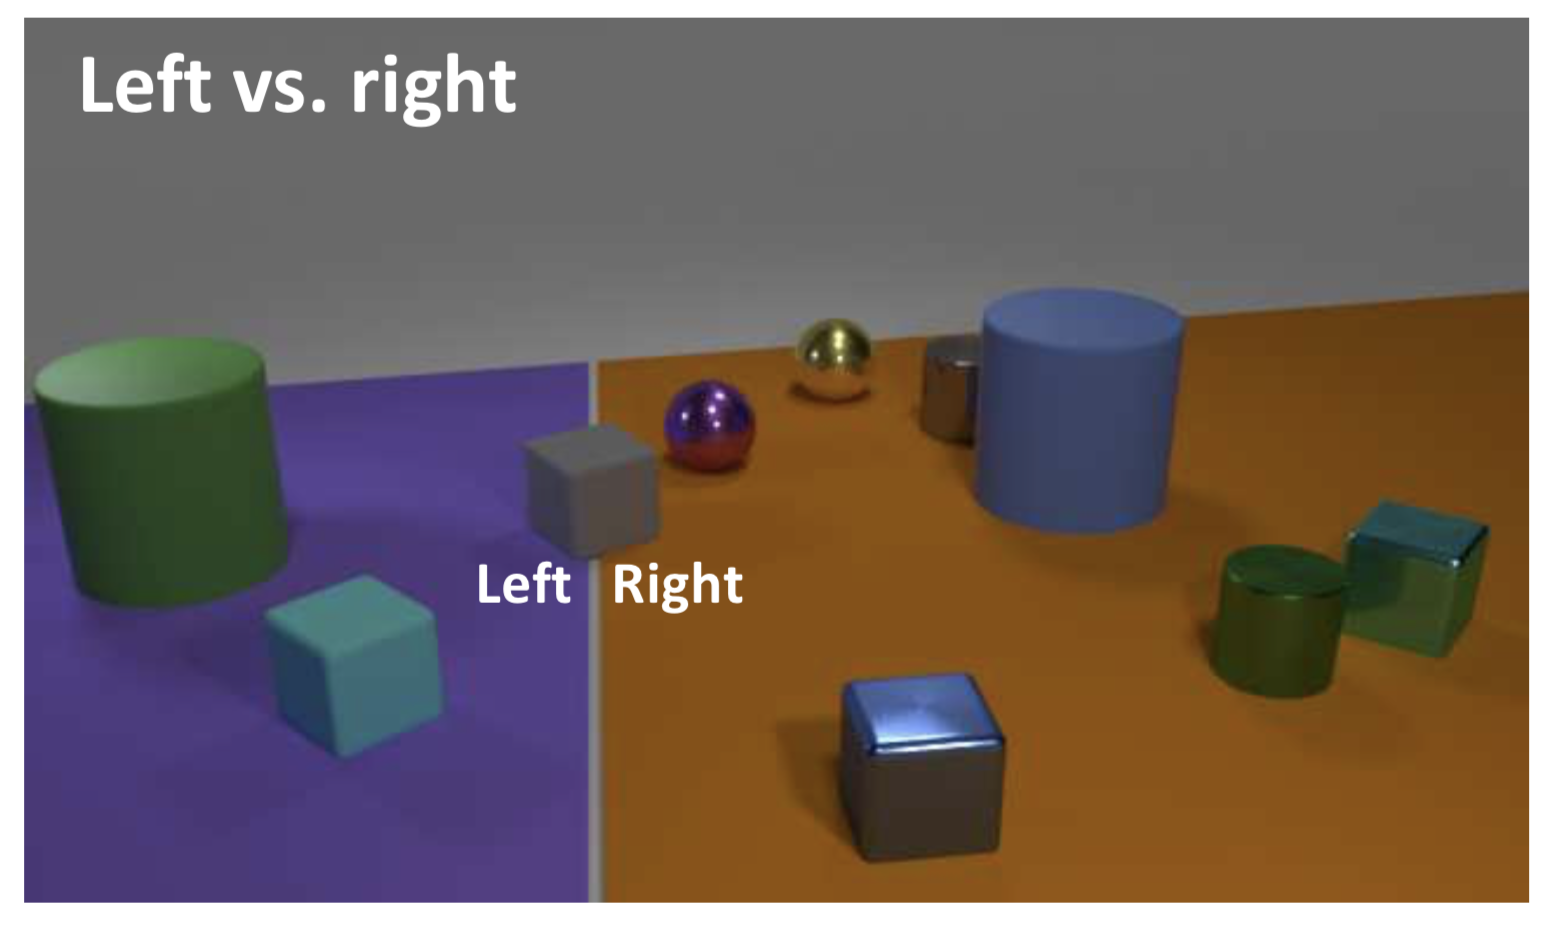
\includegraphics[width=0.3\textwidth]{clevr2.png}}
% 	\subfigure[空间前后的标注]{
% 		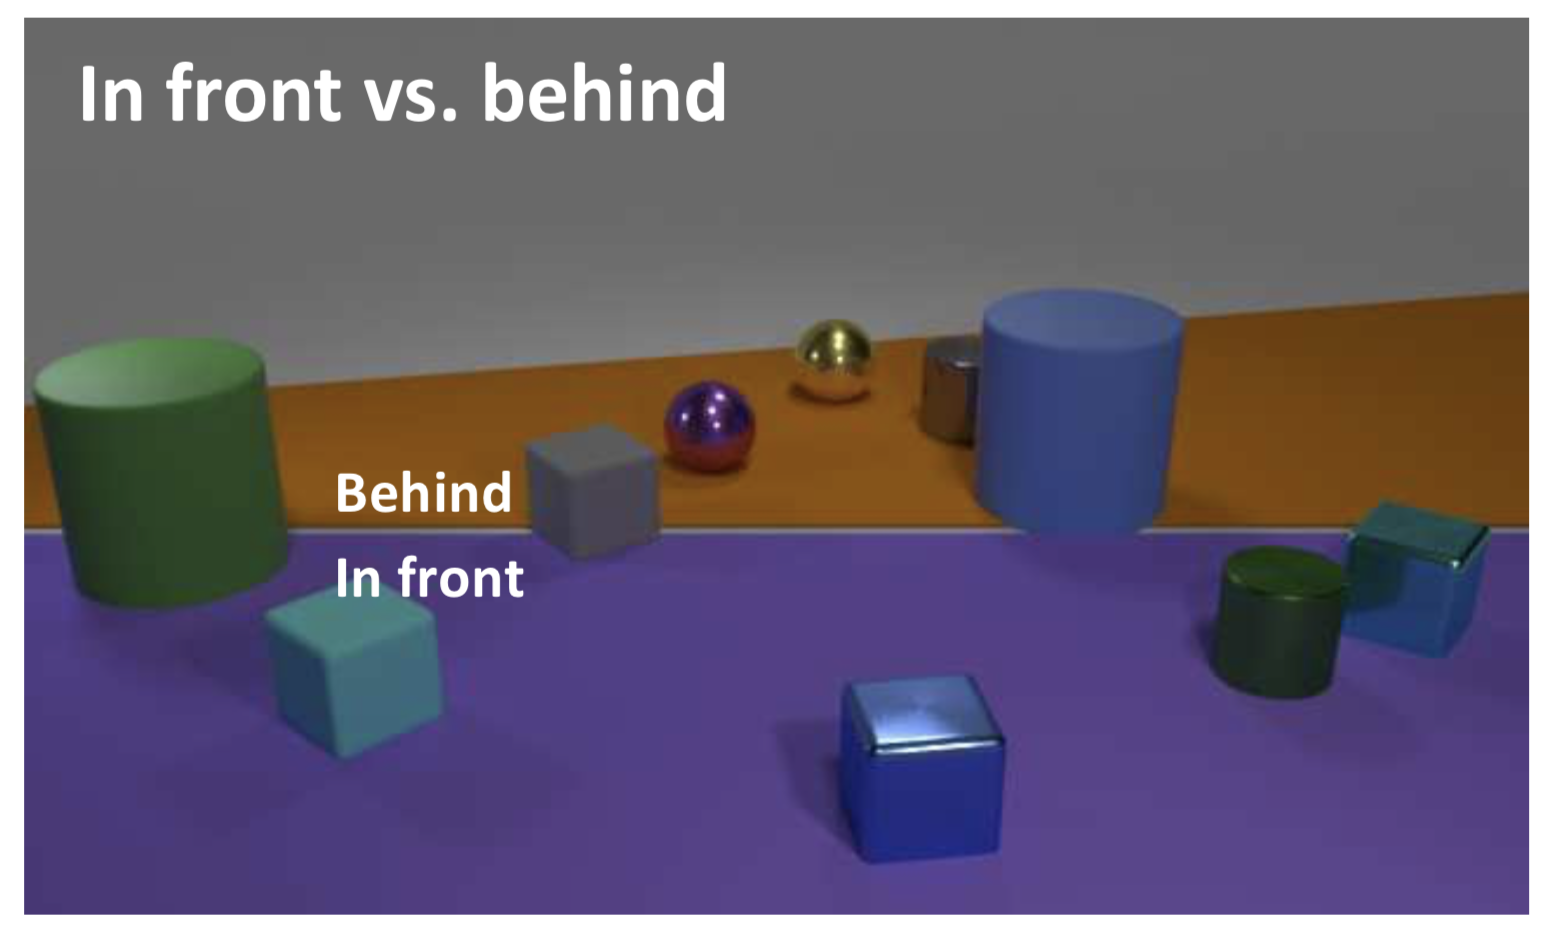
\includegraphics[width=0.3\textwidth]{clevr3.png}}
% 	\caption{CLEVR中图像标注}
% 	\label{clevr}
% \end{figure}

% \subsection{VQA-CP}
% 数据集一般会划分为训练集和测试集两个部分,在视觉问答任务中同样如此。如果训练集中的答案分布存在偏见,且测试集与训练集之间的答案分布相近,那么系统便可以通过记忆在训练过程中得到的数据偏见,并将其应用于测试过程,这样得到的准确率的可信度将会打折扣,例如,在训练集中询问颜色的问题中“白色”最为常见,同样在测试集中的“白色”也为热门答案,这回干扰系统的评估结果,不清楚系统是通过正确推理得到还是”经验“得到的。

% 针对训练集和测试集中问题答案分布相似的状况,VQA-CP重新对VQA数据集和VQA 2.0进行划分,重新划分得到的训练集和测试集在每个问题类型中的答案分布均不同,例如,在训练集中询问颜色的问题中,“白色”、“红色”为最常见的答案,而在测试集中“黑色”、“粉色”为最常见的答案;对于询问运动类型的问题,在训练集中“网球”为最多的答案,而在测试集中“滑雪”为最常见的答案(如图\ref{vqa-cp})。
% \begin{figure}[H]
% 	\centering
% 	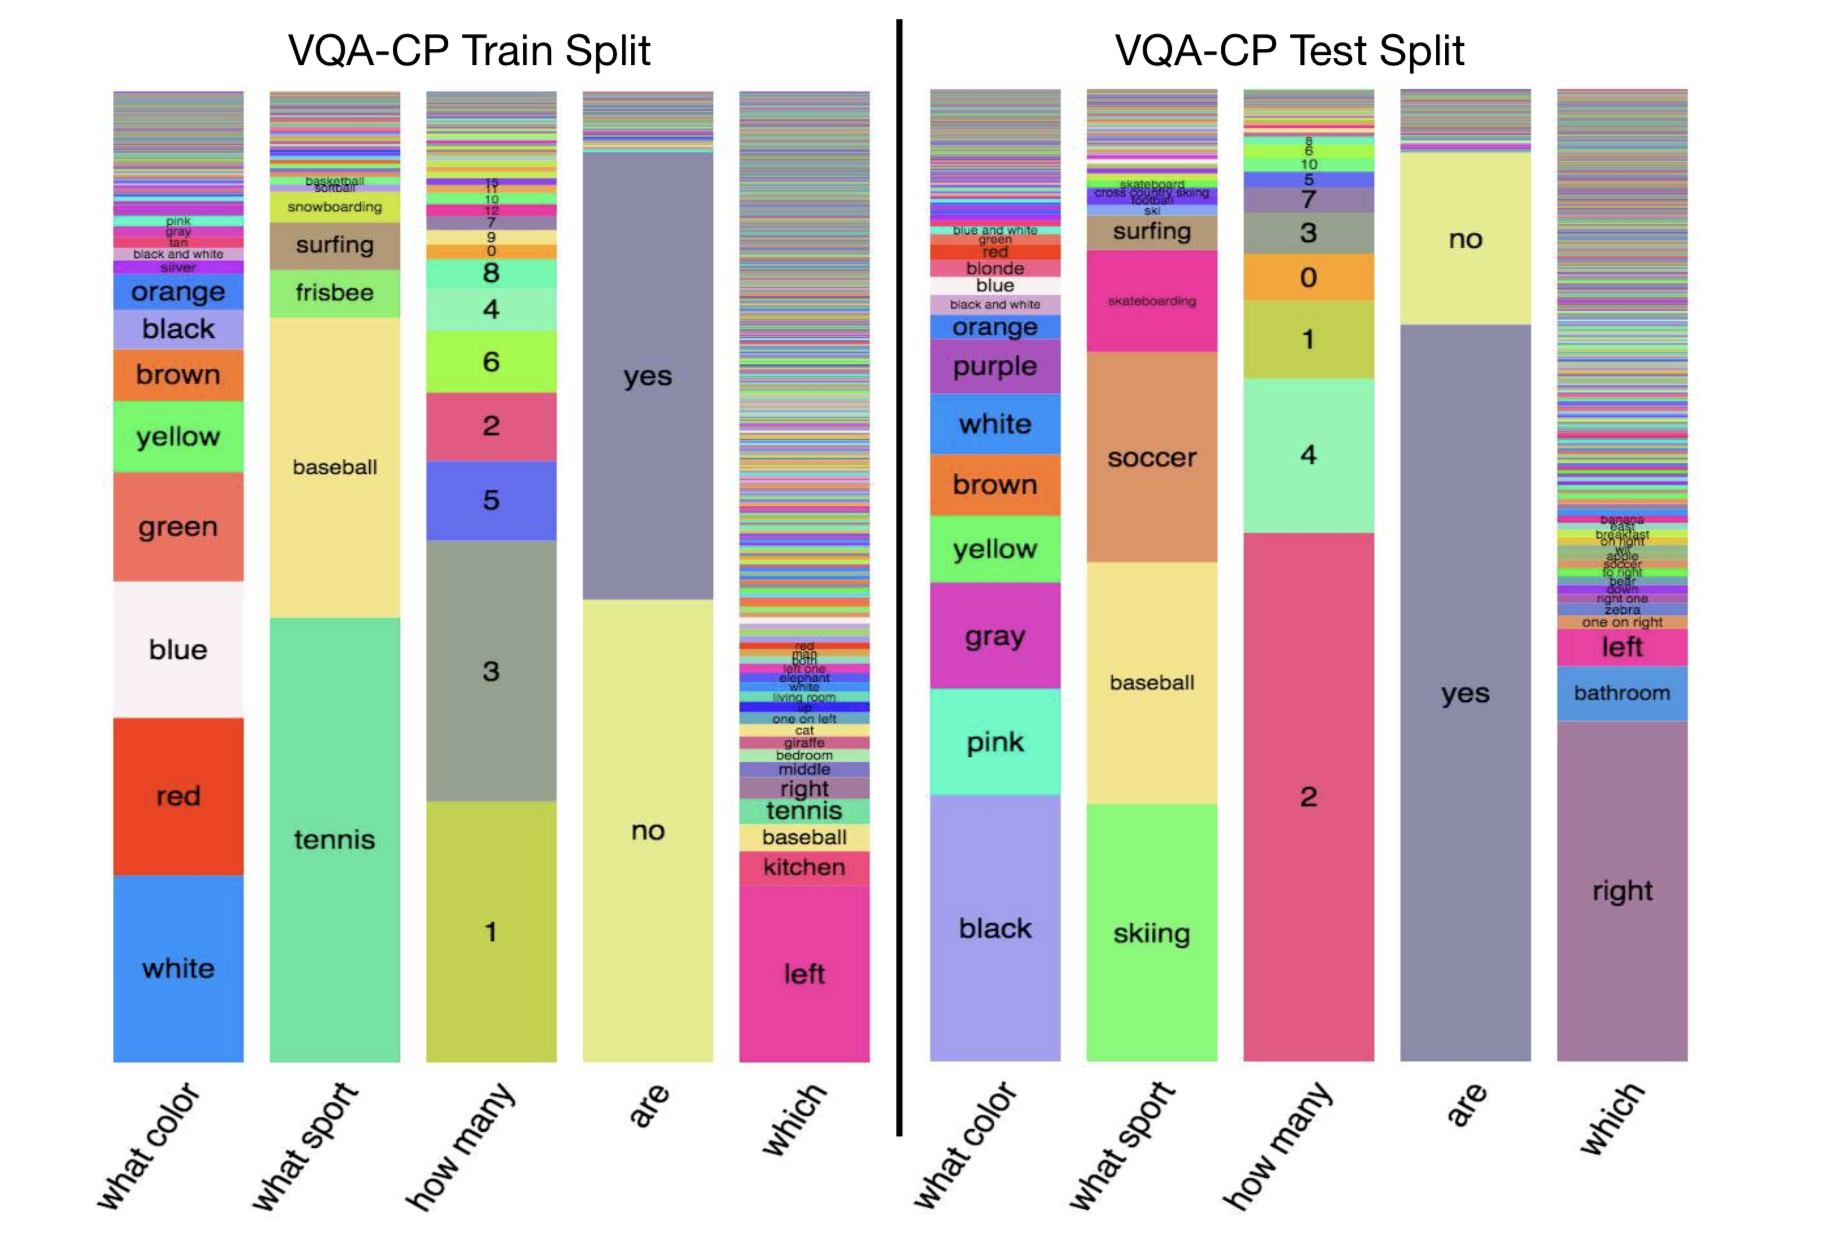
\includegraphics[width=5in]{vqa-cp.png}
% 	\caption{vqa-cp训练集和测试集的答案分布}
% 	\label{vqa-cp}
% \end{figure}

\subsubsection{基于知识的数据集}
\textbf{KB-VQA}\qquad
真实场景中的开放性问题可能涉及常识或者特定领域知识的先验知识,为了更好的评估VQA算法对需要高层次知识问题的准确推理能力,Wang等人构建了只包含复杂推理问题的数据集KB-VQA\citing{wang2015explicit}。

KB-VQA数据集从MS COCO\citing{lin2014microsoft}中挑选出700张图片样本,挑选出的图片包含150个物体类别和100个场景类别。每张图片附带有3-5个由人工生成的“问题-答案”对,所有的问题被限定在23种问题模板中,例如,“图片中是否存在某种概念?”,“图片中的某个物体被生产于什么地方?”等。
% ,详见\ref{qt}。

为了准确评估系统在需要先验知识的问题的表现,KB-VQA人工地赋予每个问题一个表示所需不同知识类型的标签,“视觉问题”、“常识问题”和“知识库问题”,其中“视觉问题”表示仅仅从图片中便可以获得答案的问题,例如,“物体是否存在于图片?”、“列出图片中包含的所有事物?”等,“常识问题”需要结合成人级别的常识和图像内容得出答案,例如,“图片涉及什么场景?”,“知识库问题”则需要某个领域特定的知识才能完成作答,例如,“图中的物品在哪一年被发明?”。数据集中的“视觉问题”、“常识问题”和“知识库问题”数量分别是1256、883和263。
% 23种问题模板在不同问题标签的分布如图\ref{qtd}。
% \begin{figure}[H]
% 	\centering
% 	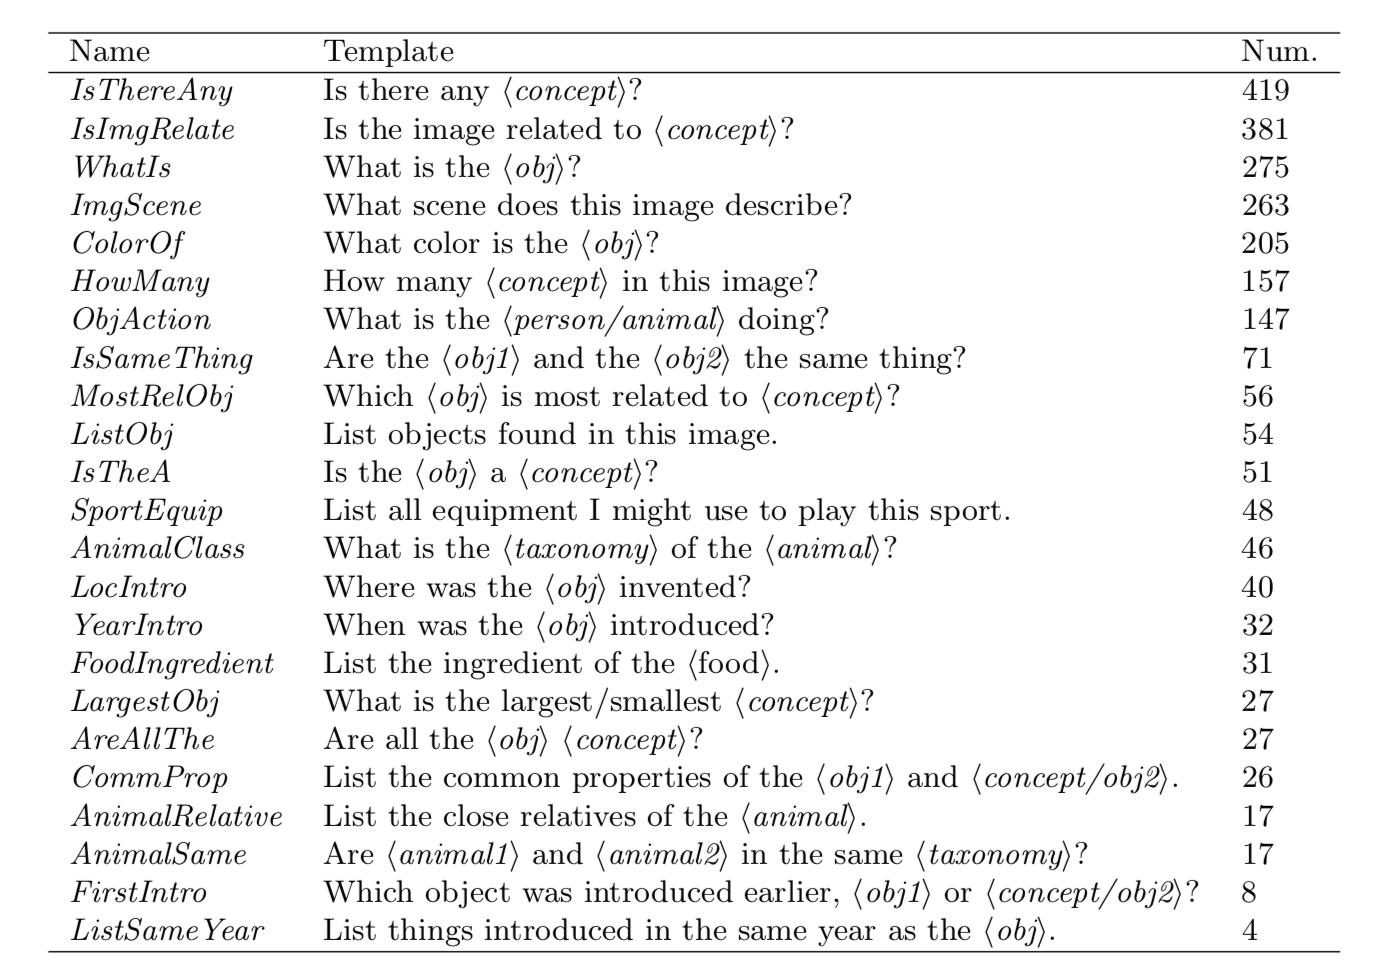
\includegraphics[width=0.8\textwidth]{qt.png}
% 	\caption{KB-VQA中23中问题模板及对应的问题数量}
% 	\label{qt}
% \end{figure}
% \begin{figure}[H]
% 	\centering
% 	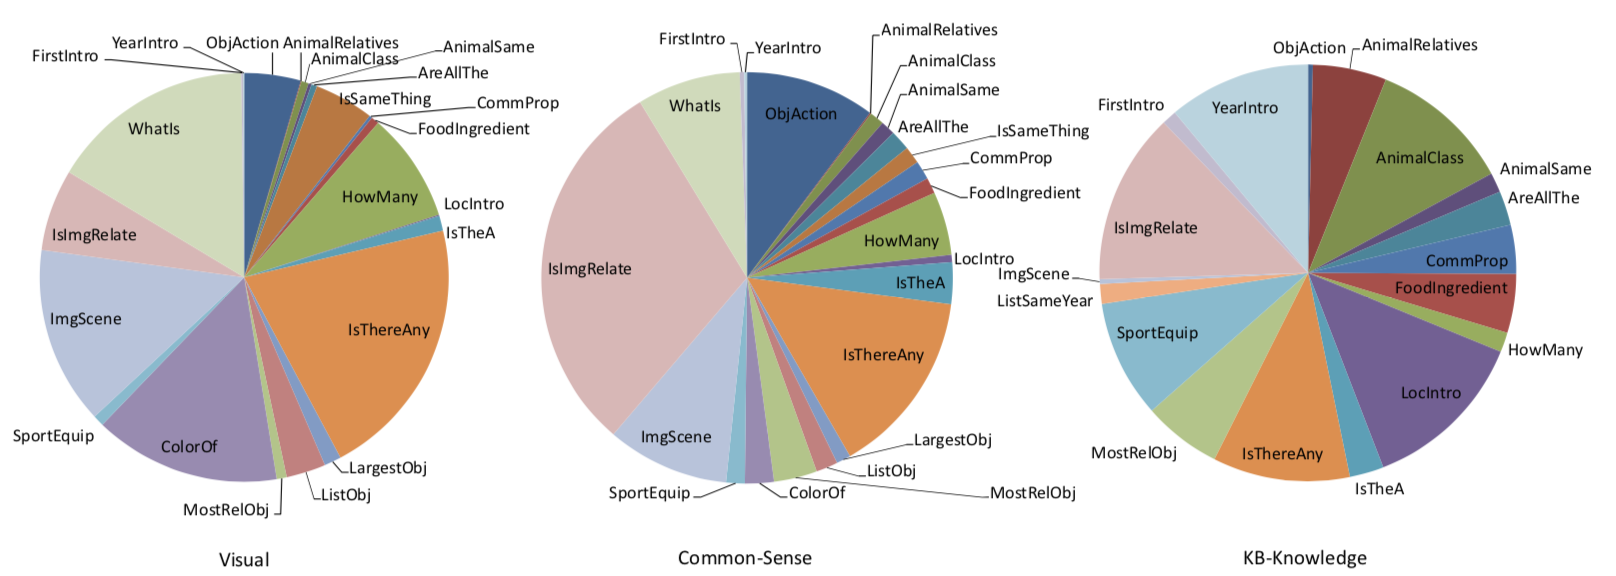
\includegraphics[width=0.8\textwidth]{qtd.png}
% 	\caption{KB-VQA中23中问题模板对应“视觉问题”、“常识问题”和“知识库问题”的分布情况}
% 	\label{qtd}
% \end{figure}

% 数据集中的“视觉问题”、“常识问题”和“知识库问题”数量分别是1256、883和263,就图片和问题的数量而言,KB-VQA数据集相较于COCO-QA等数据集是非常小的,而且从图\ref{qt}也容易看出,有16种问题类型的问题数量都不超过100个,甚至有个位数的问题数量,数据集的不均衡和小容量很难准确得评估出系统在细分问题类型上的推理能力。但需要先验知识的问题占比要远高于大型数据集,DAQUAR\citing{malinowski2014multi}几乎全是“视觉问题”,COCO-VQA\citing{ren2015exploring}仅仅包含5.5\%的问题需要常识,没有问题需要额外的知识库。

% KB-VQA在评估系统的复杂推理能力方面提供了一个解决方案,但数据集的容量、平衡性和多样性方面还需要更多的丰富,并且随着数据集的扩充,自动化和标准化的评估方式也相应的需要完善。

\textbf{FVQA}\qquad
为了评估视觉问答系统在需要先验知识的问题上的表现,Wang等人提出了FVQA数据集\citing{wang2017fvqa}。回答FVQA中的问题需要额外的知识,但不同于一般的数据集,FVQA将(图片,问题,答案)的三元组数据扩展为(图片,问题,答案,支持事实)的四元组形式,其中“支持事实”是回答问题所需要的额外知识,使用资源描述框架(RDF)的三元组形式,例如(猫,可以,爬树)。

FVQA从MS COCO\citing{lin2014microsoft}和ImageNet\citing{deng2009imagenet}中挑选出1906张图片,并对图片预处理,提取出三种类型的视觉概念:物体对象、场景和行为,最终提取出326种物体对象、21种场景和24种行为。为了获取与视觉概念相关的知识,FVQA以DBpedia\citing{auer2007dbpedia}、ConceptNet\citing{liu2004conceptnet}和WebChild\citing{tandon2014webchild}为知识源,从三种知识库中与视觉概念相关的所有知识中筛选出包含12种常见的谓语的知识,例如,关于分类的知识——“目录属于”、关于地点的知识——“地点所在”、关于大小比较的知识——“体积大于”。提取的知识以资源描述框架(RDF)的形式存储作为“支持事实”。数据集最终包含4608个需要先验知识的问题,涉及3458条事实。
% \begin{figure}[H]
% 	\centering
% 	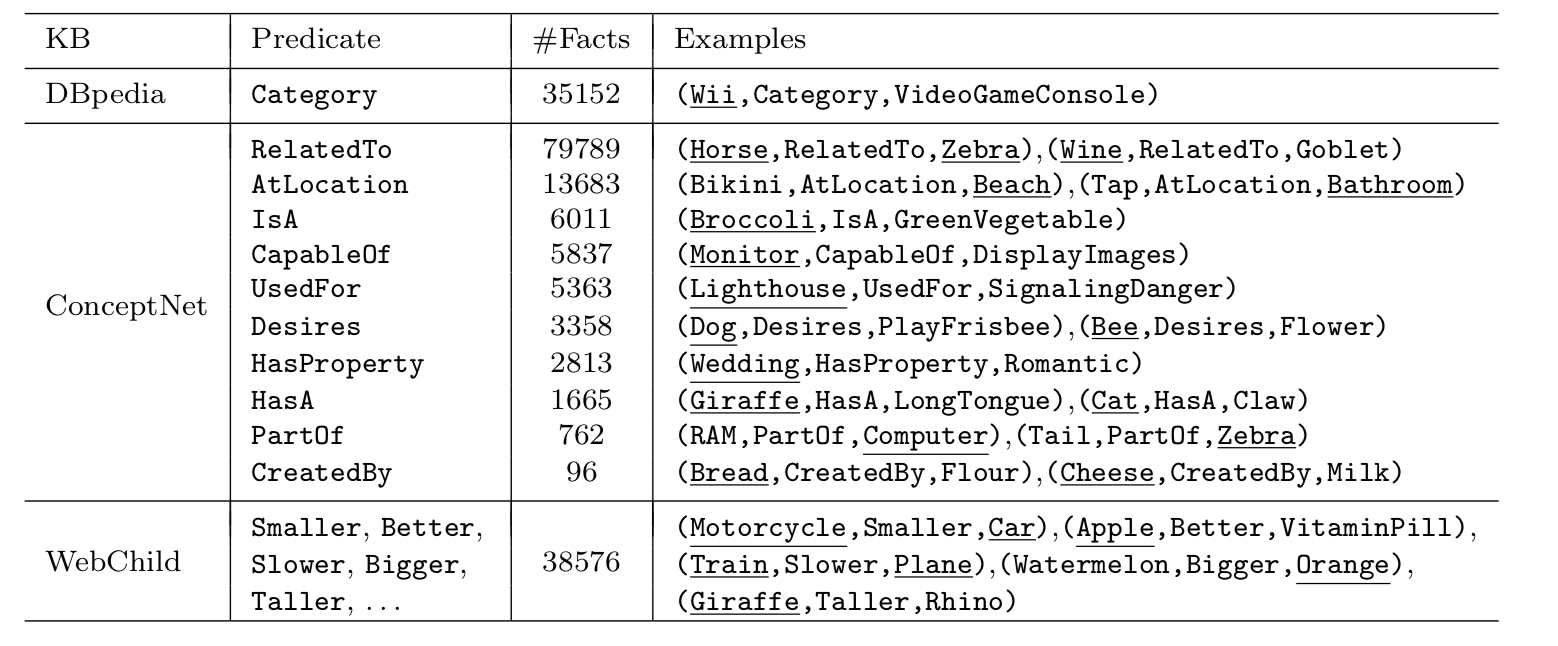
\includegraphics[width=0.8\textwidth]{fvqa_vc.png}
% 	\caption{从三种知识库中提取的知识涉及的12种谓语及相应的数量}
% 	\label{fvqa_vc}
% \end{figure}

% FVQA的问题和答案均使用人工的方式收集得到,被试者先选择图片中的一个视觉概念和一个与视觉概念相关的支持事实,再根据视觉概念和支持事实给出问题和答案,答案的来源要么是图片中的视觉概念要么是支持事实中涉及的概念。数据集最终包含4608个需要先验知识的问题,涉及3458条事实。根据视觉概念的类型,这些问题可以归为物体对象、场景和行为三种类型;根据支持事实的来源,可以归为DBpedia、ConceptNet和WebChild三种类型;根据答案来源,可以归为图片来源和知识库来源两种类型,不同分类在训练集和测试集的数量分布如图\ref{fvqa_cd}。
% \begin{figure}[H]
% 	\centering
% 	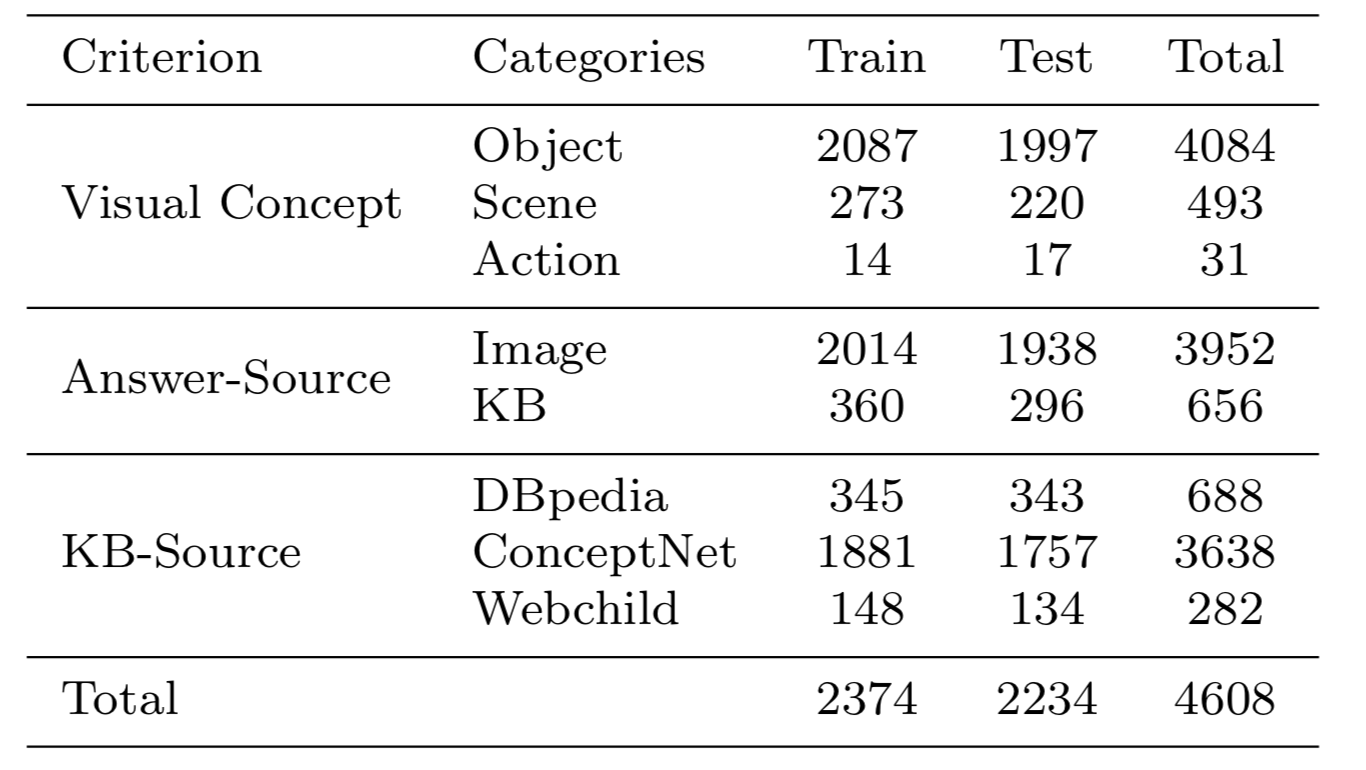
\includegraphics[width=0.8\textwidth]{fvqa_cd.png}
% 	\caption{不同分类在训练集和测试集的数量分布}
% 	\label{fvqa_cd}
% \end{figure}

% 从统计的数据上不难看出,绝大多数问题是针对图像中的物体对象,这与提供的视觉概念中物体对象的高占比有强关联,从知识来源上分析,答案除了能从图像中获得外,还包含14\%的答案需要从额外知识库中获得,并且问题中不包含“是或否”的二值问题,这降低了系统”猜中正确答案“的情况。

% FVQA和同样包含先验知识的数据集KB-VQA两者都能通过查询语言获取知识库中的数据,但不同于KB-VQA,FVQA拥更多的图片和问题数量,并且所有问题都需要额外知识。FVQA增加了ConceptNet和WebChild作为知识源,提高了知识库的多样性,能回答更多类型的问题,而不用预先设定问题模板。但FVQA数据集中几乎所有的答案都是物体对象,且为单个词语,不能训练模型给出对象关系的答案。FVQA数据集的支持事实多为单一谓语的句子,句式结构简单,如果用做训练集,不能考察模型应对多动词结构问题时的答案正确率。

% 然而两个数据集都面临着同样的问题:数据量的扩充和问题类型的扩充。两个数据集的问题收集都是通过人工的方式,并且参与者数量有限,因此直接导致了问题数量远低于其他自动化方法生成的数据集。大规模的协同工作和探索更多自动化方法是扩充数据集容量的方向。两个数据集都受到问题类型的限制,KB-VQA使用预先设定的问题模板,限制了问题的开放程度,FVQA虽然没有使用预先设定的问题模板,但其筛选的12种谓语间接的限制了问题的类型。

\section{视觉问答模型架构}
视觉问答任务要求系统能同时正确理解问题文本内容和图像内容,从视觉问答的处理过程可以看出,算法的核心有三个部分组成:如何提取出高层次的图像特征,例如,物体、属性、场景等;如何挖掘问题文本中的语义信息,以求能深入的理解问题内容,确定答案的形式和内容;如何结合图像特征和文本特征,得出正确或是最佳答案。

受神经网络在计算机视觉和自然语言处理成功应用的影响,从2014至今的视觉问答研究多采用了神经网络模型,并且模型基本上都由特征提取、注意力机制、特征融合、答案生成四个部分组成。模型使用卷积神经网络CNN提取图像特征,使用循环神经网络RNN或者长短期记忆LSTM处理文本信息,再通过不同的注意力机制增强特征的表达能力,最后融合特征,使用分类器输出答案,整体架构如图\ref{answer-generation}所示。
\begin{figure}[H]
	\centering
	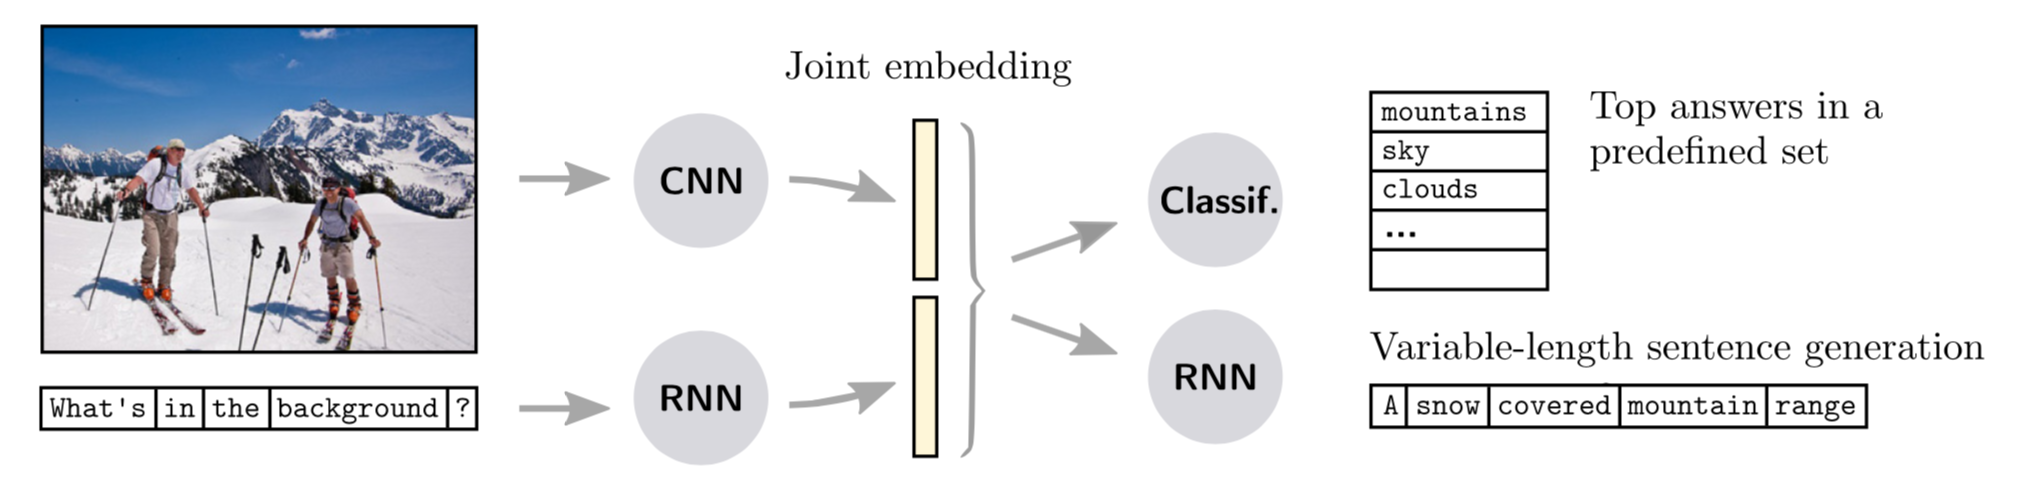
\includegraphics[width=0.8\textwidth]{answer-generation.png}
	\caption{VQA模型的一般架构}
	\label{answer-generation}
\end{figure}

% (1)特征提取部分一般由图像特征提取和文本特征提取两个部分组成,但一些引入知识库的模型中,可能会添加一个知识库特征提取部分,用于丰富特征。图像特征提取的方法一般使用预训练的卷积神经网络,例如VGGNet\citing{simonyan2014very}、 ResNet\citing{he2016deep}、GoogLeNet\citing{Szegedy_2015_CVPR}、Faster R-CNN\citing{ren2015faster}等。问题文本的特征提取则借鉴了自然语言处理中的成果,例如词袋模型(CBOW)\citing{zhou2015simple}、长短期记忆(LSTM)\citing{malinowski2015ask}、门控复发单位(GRU)\citing{noh2016image,kumar2016ask,xiong2016dynamic}。

% (2)注意力机制的引入也是跟随图像处理和自然语言处理的成功应用,通过对图像或文本特征不同部分分配有差异的权重值,从而更新特征,聚焦特征中重要的局部,实现特征增强。注意力机制能有效的抑制全局噪音,减少模型的无关运算,从而提高模型的准确性,在众多应用中均证明了其有效性。

% (3)特征融合是将提取得到的图像特征和文本特征映射到同一向量空间,并使用通过特征向量串联\citing{zhou2015simple}、卷积\citing{ma2016learning}、逐元素相乘\citing{antol2015vqa}、逐元素相加\citing{malinowski2015ask}等方法融合跨模态特征,便于后续的分类预测。对于视觉问答任务而言,图像特征和文本特征具有异质性,数据来源和特征分布都不同,因此好的特征融合对于模型的准确性具有重要的意义。

% (4)答案生成是解码融合后的特征,输出答案的部分。在视觉问答模型中,系统输出答案的方式有两种,最常见的方式是将任务视为分类问题,根据候选项的概率大小,确定答案。第二种方式则直接由系统合成答案语句,此类方法多出现在有额外知识库的视觉问答系统中,例如Attributes-LSTM\citing{wu2016value}、ACK\citing{wu2016ask}、Ahab\citing{wang2015explicit}、Facts-VQA\citing{wang2017fvqa}、Multimodal KB\citing{zhu2015building}。

\subsection{特征提取}
特征提取部分一般由图像特征提取和文本特征提取两个部分组成,但一些引入知识库的模型中,可能会添加一个知识库特征提取部分,用于丰富特征。图像特征提取的方法一般使用预训练的卷积神经网络。问题文本的特征提取则借鉴了自然语言处理中的成果,例如词袋模型(CBOW)\citing{zhou2015simple}、长短期记忆(LSTM)\citing{malinowski2015ask}、门控复发单位(GRU)\citing{noh2016image,kumar2016ask,xiong2016dynamic}。

\subsubsection{图像特征提取}
在卷积神经网络出现以前,图像的特征提取一般是使用人工设计特征,例如SIFT\citing{lowe1999object}、HOG\citing{dalal2005histograms}。虽然这些特征在特定任务上表现良好,但是其泛化性能较差,这意味着特征提取的成本较高。而卷积神经网络是一种深度学习模型,具有分层特征学习能力,以及更好的识别和泛化性能\citing{zeiler2014visualizing}。

卷积神经网络从机器视觉的成功应用开始,成为一众人工智能子领域的研究模型,已经被广泛用于物体检测、姿态检测、自然语言处理、语音识别等领域。并且随着迁移学习的兴起,大量性能优异的预训练卷积神经网络被用于图像特征提取,例如AlexNet\citing{krizhevsky2012imagenet}、VGGNet\citing{simonyan2014very}、 ResNet\citing{he2016deep}、GoogLeNet\citing{Szegedy_2015_CVPR}等。虽然有大量新的卷积神经网络被提出,但是它们都使用输入层、卷积层、池化层、全连接层和分类层组成的基本架构,如图\ref{cnn_structure}所示。
\begin{figure}[H]
	\centering
	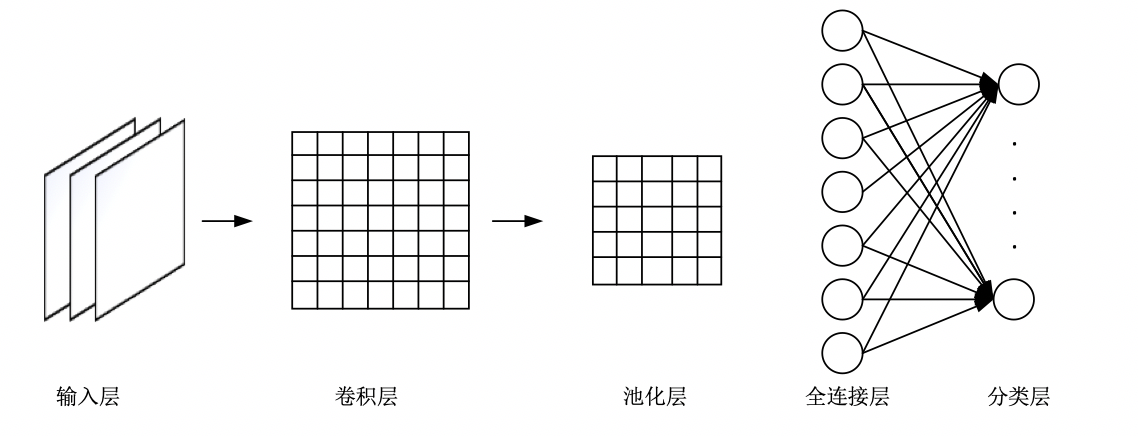
\includegraphics[width=0.8\textwidth]{cnn_structure.png}
	\caption{卷积神经网络的基本结构}
	\label{cnn_structure}
\end{figure}

卷积层是卷积神经网络的核心组成。对于高像素的彩色照片,全连接的神经网络将会产生大量参数,巨量的参数不利于模型的训练。卷积层的节点通过卷积核采样特征图的局部,并对局部的特征值进行卷积操作,再通过平移卷积核在特征图上滑动,从而扫描整张图片。不同的卷积核能够捕获图像的不同层次的特征,底层的卷积核得到的是边缘、颜色、纹理等粗粒度的特征,高层的卷积核则得到抽象的语义信息。给定输入图像I,$H_i$表示第i个卷积层的特征图,其中$H_0=I$,则相邻卷积层的特征图满足关系:
\begin{equation}
H_i = f(H_{i-1}\otimes W_i + b_i)
\end{equation}
其中,$W_i$表示第i层卷积核的权重向量,$b_i$表示第i层卷积核的偏置,$\otimes$表示卷积操作,$f$为非线性激活函数。常见的激活函数有Sigmoid, tanh, ReLu, Leaky ReLu, Maxout等,其中ReLu的公式为:
\begin{equation}
f(x) = max(0,x)
\end{equation}
因为其具有计算量小、收敛快等优点,被广泛用作激活函数。

池化层紧跟卷积层,对特征图进行下采样,降低特征维度,一方面能减少网络的计算复杂度,加快收敛,另一方面能提取主要特征。常见的池化方式有平均池化和最大值池化。

通过多个交替的卷积层和池化层后,特征进入全连接层和分类层,对每个类别进行概率预测,得到概率分布$Y$($l_i$表示第i个标签的类别)。因此整个卷积网络可以被视为接受输入$H_0$,在网络参数$W, b$的条件下,得到正确类别i的函数,如下式,
\begin{equation}
Y(i)=P(L=l_i | H_0; (W, b))
\end{equation}

网络的训练目标是最小化损失函数$L(W, b)$,从而更新模型参数。常见的损失函数均值平方、二值交叉熵、softmax交叉熵等。

\subsubsection{文本特征提取}
和众多自然语言处理任务一样,在视觉问答任务中如何准确理解问题内容对最终的答案准确率上有着决定性的影响。而自然语言理解中最为基本和核心的便是文本表达,文本表达将自然语言转换为计算机可处理的数字,为自动化处理文本相关的任务建立了基础。

在文本表达中,独热向量(one-hot)是最早也是最为简单的词向量。但是其稀疏性会带来的“维度灾难”和因简单的编码方式而造成“语义鸿沟”。基于分布式假设——即处于相似上下文的词语具有相似的含义,研究者先后提出了多种使用分布式表示的词向量模型,例如,CBOW,Skip-Gram,word2vec\citing{mikolov2013distributed},LSTM\citing{10.1162/neco.1997.9.8.1735}、潜在语义分析(LSA)\citing{landauer1998introduction},GloVe\citing{pennington2014glove}。

CBOW和Skip-Gram均是使用神经网络模型训练上下文信息得到词向量。word2vec也使用了CBOW与Skip-Gram来训练模型与得到词向量,但是并没有使用传统的DNN模型,而是使用霍夫曼树来代替隐藏层和输出层的神经元,提高了计算效率,因此被研究者广泛地使用作为预训练的词向量。但是由于word2vec使用滑动窗口来限定上下文信息,因此得到的词向量仅仅使用了局部的语义和语法信息。

循环神经网络(RNN)是处理序列化数据最为常用的模型,通过将句子中词特征循环迭代后,得到句子特征。但由于循环神经网络具有遗忘性,存在长时依赖问题,长短期记忆神经网络(LSTM)逐渐替代RNN。LSTM由三个门控制,分别是输入门、遗忘门和输出门。输入门控制着网络的输入,遗忘门控制着记忆单元,自动学习需要保存的记忆,输出门控制网络的输出。

不同于word2vec使用局部语料,潜在语义分析(LSA)采用统计计数的方式获得语料的全局信息,其统计预料库中每两个词共同出现的次数构成共现矩阵,并采用了基于奇异值分解(SVD)的矩阵分解技术对大矩阵进行降维,得到词向量。然而LSA方法中的SVD计算量很大,并且共现矩阵仅能表示两个词语同时出现的次数,并不能表示词语之间的远近关系。

为了改进word2vec的局部预料限制和LSA的计算复杂性,GloVe使用衰减函数改造LSA的共现矩阵,使得词语间的远近关系得以表达。GloVe还构建了词向量和共现矩阵之间的近似关系,使用梯度下降算法取代了LSA中的奇异值分解,大大减少了计算代价,并且得到了远超LSA和word2vec的性能。

以上提及的文本特征化方法被广泛的使用在视觉问答模型中。值得注意的是,以上方法都是将文本转换为固定的静态词向量,而静态词向量缺乏对上下文的感知,因此不能有效的表征多义词和具有多语法成分的词组。本文的重要改进之一便是引入动态词向量,具体内容将在N-KBSN模型架构中介绍。

\subsection{注意力机制}
人类获取外部视觉信息时,会自动形成一种“像素不均衡”,在同一视野范围内的像素被视觉中枢神经系统根据“关注区域”的远近、相关性特征自动分配不同的分辨率,使得“关注区域”内的像素具有极高的分辨率,而其他的像素仅仅作为视觉信息输入,并不参与大脑的语义处理(如图所示\ref{human-virtual})。因此视觉注意力机制帮助大脑过滤了低相关性的视觉信息,减少了待处理数据的体积,极大地提高了信息处理速率并松弛了大脑负载。
\begin{figure}[H]
	\centering
	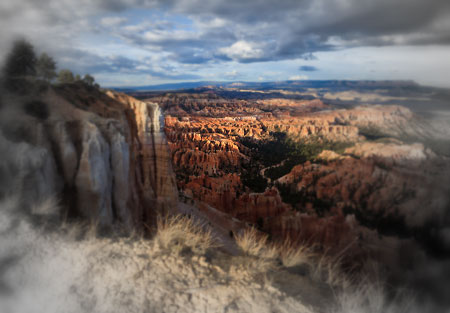
\includegraphics[width=0.5\textwidth]{human-virtual.png}
	\caption{人类视觉系统的“像素不均匀”现象}
	\label{human-virtual}
\end{figure}

近几年,受到人类视觉注意力机制的启发,在神经网络中引入注意力机制变得十分热门,在自然语言处理和计算机视觉领域的应用也极大得帮助了原有算法精度和计算效率的提升。Google Deepmind团队提出了一种带有注意力机制的循环神经网络(RNN),并成功应用于图像分类任务,获得了优于以往卷积神经网络(CNN)的基线水平的分类精度\citing{mnih2014recurrent}。随后,带有注意力机制的循环神经网络便被广泛应用于自然语言处理和计算机视觉的多个子领域\citing{bahdanau2014neural, xu2015show, NIPS2015_5847}。Bahdanau等人将注意力机制引入神经机器翻译任务,仍然使用“编码-解码”的翻译模式,但一改以往将源语言文本映射为一个固定长度的向量的编码方式,而是将原语言文本编码为向量序列,解码时将翻译和位置对应因素联合学习,训练向量序列中各向量对翻译词组的不同权重,加和完成翻译结果的推断,得到了以往最优的结果\citing{bahdanau2014neural}。Xu等人受到注意力机制在机器翻译和物体识别任务成功应用的启发,将带有注意力机制的循环神经网络应用于自动生成图像标注,并且在Flickr9k, Flickr30k 和MS COCO 三个数据集上均获得了最优的结果\citing{xu2015show}。随后,更多注意力机制的变型或优化研究均在图像标注任务上展开\citing{ 7243334, wu2017global, li2017image, lu2017knowing}。

相较起图像标注任务,视觉问答任务除了要求系统能理解图片内容,生成语义和句式合理的自然语言文本以外,还需要联合学习问题文本和聚焦与问题相关的图像细节。因此,在视觉问答模型中,从作用对象来分,注意力机制可以分为图像自注意力机制、文本自注意力机制、引导注意力机制。不同的模型使用的注意力机制细节不同,本文将使用多头注意力机制(Multi-head Attention, MA)实现图片的自注意力(V-SA)、问题文本的自注意力(Q-SA)、由问题引导的对图像的注意力(Guided Attention, GA),具体的实现细节详见N-KBSN模型。

\subsection{特征融合}
对于视觉问答任务而言,图像特征和文本特征具有异质性,数据来源和特征分布都不同,因此好的特征融合对于模型的准确性具有重要的意义。

多模态的融合方式可以分为协同表示和联合表示,协同表示是指将一种模态特征映射到另一种模态的特征空间,再融合;联合表示则是将不同模态的特征映射到同一特征空间。具体而言,协同表示是将图像特征映射到文本特征空间,再使用各类特种融合方法;联合表示则分别提取图像特征和文本特征,并且将两种特征统一维度,再进行相加或者拼接。联合表示的方式具有很高的灵活性,图像和文本特征的提取分开,并且融合的方式的选择也更为多样,因此目前大多模型均是使用该模式,本文也是使用联合表示,分别提取特征,再融合。

常用的特征融合方法有:向量串联\citing{zhou2015simple}、卷积\citing{ma2016learning}、逐元素相乘\citing{antol2015vqa}、逐元素相加\citing{malinowski2015ask},另有模型使用更复杂的特征融合方法,例如,动态参数层\citing{noh2016image}、多模态紧凑双线性池化方法(MCB)\citing{fukui2016multimodal}。

\subsection{答案生成}
答案生成是解码融合后的特征,输出答案的部分。在视觉问答模型中,系统输出答案的方式有两种,最常见的方式是将任务视为分类问题,根据候选项的概率大小,确定答案。第二种方式则直接由系统合成答案语句,此类方法多出现在有额外知识库的视觉问答系统中,例如Attributes-LSTM\citing{wu2016value}、ACK\citing{wu2016ask}、Ahab\citing{wang2015explicit}、Facts-VQA\citing{wang2017fvqa}、Multimodal KB\citing{zhu2015building}。

\section{本章小结}
本章从视觉问答任务的定义、问题类型和数据集三个方面介绍该领域的基本知识,其中,我们提出了一种按照答案与问题和图像相关性的问题分类标准。本章还介绍了视觉问答模型的一般架构,并从图像特征提取、文本特征提取、注意力机制、特征融合、答案生成五个方面展开说明了目前的实践情况以及原理和公式。


\chapter{基于动态词向量的联合嵌入模型}
视觉问答来的研究受到机器学习算法在自然语言处理和图像识别等领域成功应用的启发,因此从2015年视觉问答任务出现至今,大量的VQA模型都使用了联合嵌入模型,使之成为目前视觉问答的的主流模型。顾名思义,联合嵌入模型是将任务的源信息——图像和问题文本——表示为向量,再通过特征融合,将不同模态的信息映射到统一的向量空间,最终从联合表征中提取出答案。因为这种架构的模型易于训练,研究者采用不同的图像特征的提取方法、不同的文本特征的提取方法、两种模态的不同融合方法,做了许多尝试。

Antol等人在2015年发布了开放问题的视觉问答数据集VQA\citing{antol2015vqa}之后,在数据集的基础上提出了VQA挑战。VQA挑战中涌现了大量视觉问答模型,模型的准确率也逐年升高,图\ref{vqa_challenge}展示了2015年-2019年VQA挑战中的最优模型的准确率。通过研究其中表现优异的模型,我们发现几乎所有模型都使用了联合嵌入模型,并且加入注意力机制之后准确率能够进一步提升,例如,四年的冠军模型都是使用了注意力机制的联合嵌入模型,其中2019年的冠军模型\citing{Yu_2019_CVPR}能在VQA2.0数据集下获得总体75\%作用的准确率,相较于四年前的模型准确率得到了20\%的提升,并且距离人类表现也只有5\%左右的差距。
\begin{figure}[H]
	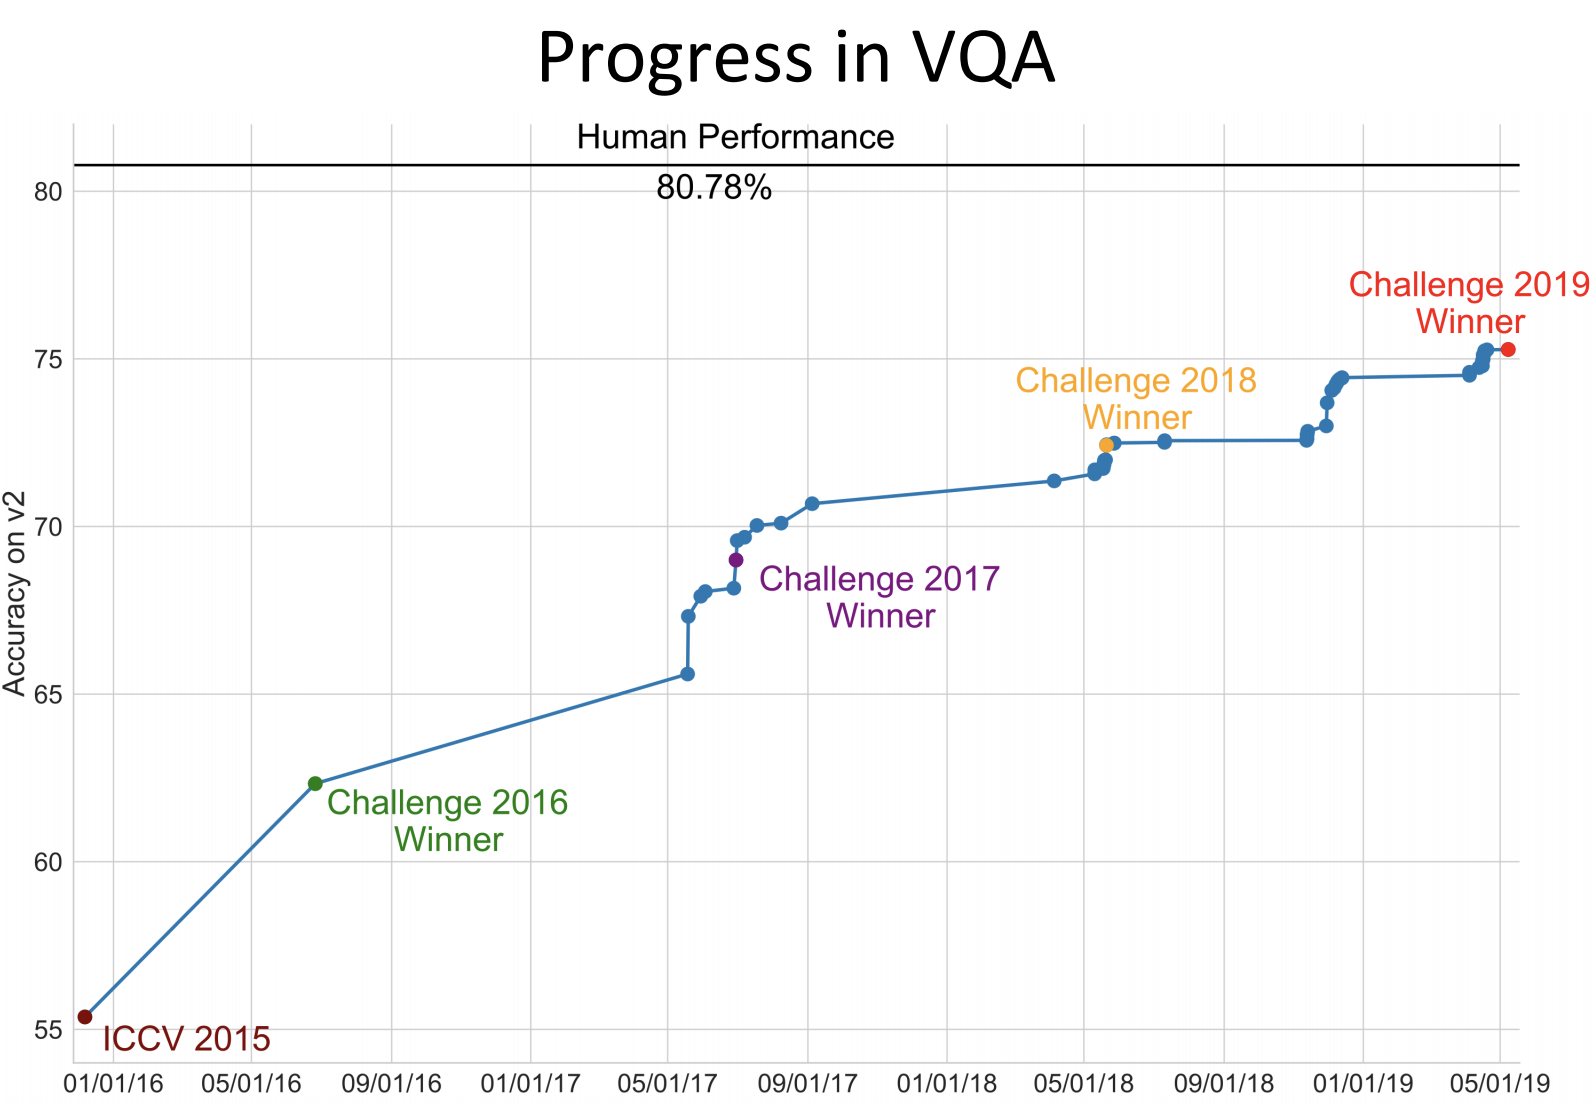
\includegraphics[width=0.7\textwidth]{vqa_challenge.png}
	\caption{VQA挑战中模型的准确率曲线}
	\label{vqa_challenge}
\end{figure}

我们认为联合嵌入模型在VQA挑战的优异表现有以下几点原因。
\begin{itemize}
  \item [1)] 
  引入注意力机制。2016年的优胜模型\citing{ilievski2016focused}提出“动态关注注意力(FDA)”模型,目的是根据问题中的关键词动态的对图像的不同区域分配带有权重的注意力,得到图像的全局特征和局部特征的结合。2017和2018年的优胜模型都使用论文\citing{anderson2018bottom}中的自上而下和自下而上的图像注意力机制,2019年的优胜模型使用了Transformer\citing{NIPS2017_7181}的多头注意力机制。注意力机制的引入能够减少无关特征的干扰,提高计算效率,并且一定程度的提高可解释性。
  \item [2)]
  VQA2.0数据集的局限性。VQA挑战以VQA2.0为数据集,然而根据我们提出的依照答案和源信息统计相关性的标准(详见表\ref{ques_type}),VQA2.0中需要常识或者外源知识的qi类型仅仅占所有问题的5.5\%\citing{wang2015explicit},这意味着回答绝大多数的问题都不需要额外的信息。然而在现实中的开放性问题中,涉及常识或者外源知识的问题广泛存在,因此VQA2.0数据集存在局限性,而这种局限性使得模型只需要关注图像和文本,因此联合嵌入模型成为了主要架构。
  \item [3)]
  得益于图像识别和自然处理模型的进步。联合嵌入模型具有灵活的组合模式,很容易从将其他任务中表现优异的模型迁移过来形成新的模型。
\end{itemize}

我们对具有代表性的联合嵌入模型,按照图像特征化方法、文本特征化方法、特征融合方法、VQA2.0的准确性、是否使用静态词向量,总结为表\ref{model_compar}。
\begin{table}[H]
% \resizebox{0.8\textwidth}{!}{}
\centering
\caption{代表性联合嵌入模型的比较}
\resizebox{\textwidth}{!}{
\begin{tabular}{llllll}
\toprule
\textbf{模型} & \textbf{图像特征化} & \textbf{文本特征化} & \textbf{特征融合} & \textbf{VQA准确率(\%)} & \textbf{静态词向量} \\
\midrule
LSTM Q+I \citing{antol2015vqa}&  VGGnet& LSTM&  逐项点乘&  54.1& 是\\
iBOWIMG\citing{zhou2015simple}&  GoogleNet& 词袋模型&  串联&  55.9& 是\\
DPPNet \citing{noh2016image}&  VGGnet& GRU&  动态参数层&  57.4& 是\\
D-CNN\citing{ma2016learning}&  CNN& CNN&  CNN&  58.4& 是\\
MCB\citing{fukui2016multimodal}&  RestNet& LSTM&  MCB&  64.2& 是\\
2017-winer\citing{teney2018tips}&  Faster R-CNN& Glove+GRU&  逐项点乘& 69.87 & 是\\
2018-winer\citing{anderson2018bottom}&  Faster R-CNN& Glove+GRU&  逐项点乘& 72.27 & 是\\
2019-winer\citing{Yu_2019_CVPR}&  Faster R-CNN& Glove+LSTM&  MLP& 75.26 & 是\\
\bottomrule
\end{tabular}}
\label{model_compar}
\end{table}

如上表所示,现有的联合嵌入模型采用了不同的图像特征化、文本特征化、特征融合方法的组合,但是所有现有的模型的文本特征化均使用静态词向量。静态词向量使用一个语料库作为数据集,训练得到每个词语的分布式表示,这种表示方法的优点在于词语的向量预先训练得到,因此应用于不同的下游任务时,无需再训练,提高了运算效率。然而在真实的语言环境中,同一词语在不同的语境中表示不同的含义,也可能作为不同的语法成分,而这些差异并不能被静态词向量表示,因此可能出现语义和语法的偏差。

为了解决静态词向量的问题,我们构建了一个基于动态词向量的联合嵌入模型——None KB-Specific Network(N-KBSN)模型。本章将重点介绍N-KBSN模型,并且使用VQA2.0数据集训练。N-KBSN由三个主要部分组成:问题文本和图像特征提取模块、自注意力和引导注意力模块、特征融合和分类器。其中,图像特征提取使用在多目标检测中表现优秀的Faster R-CNN\citing{ren2015faster},问题文本特征提取使用能够获得上下文信息的ELMo模型\citing{Peters:2018},并使用从Transformer中借鉴的多头注意力机制\citing{NIPS2017_7181}分别实现图片的自注意力(V-SA)、问题文本的自注意力(Q-SA)、由问题引导的对图像的注意力(Guided Attention, GA),最后通过特征融合预测答案。N-KBSN模型的基础架构如图\ref{N-KBSN}。
\begin{figure}[H]
	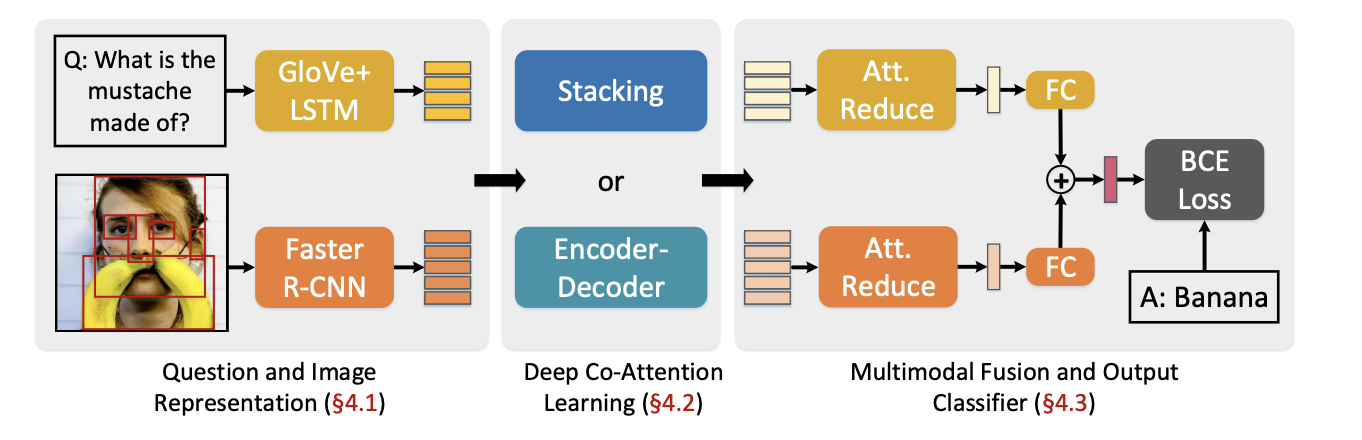
\includegraphics[width=0.8\textwidth]{N-KBSN.png}
	\caption{N-KBSN基础结构}
	\label{N-KBSN}
\end{figure}

\section{基于Faster R-CNN的图像特征化}
目标检测是机器视觉领域的重要应用之一,目标检测的核心任务是准确、快速的从图像中定位出目标并且能识别目标的类别、属性等特性。传统的目标检测算法通过滑动窗口的方式选取区域选择、提取特征提并分类,例如可变形的组件模型(DPM)方法\citing{felzenszwalb2009object}等。这些传统的目标检测算法大多区域选择的策略效果差、时间复杂度高,并且因为由于是人工提取特征,提取的特征层次较低,致使模型的鲁棒性较差。由于深度学习在视觉问答任务的优异表现,大批优秀的目标检测算法出现,例如R-CNN\citing{girshick2014rich}、SPP-Net\citing{he2015spatial}、Fast R-CNN\citing{girshick2015fast}、Faster R-CNN\citing{ren2015faster}、Mask R-CNN\citing{he2017mask}、YOLO\citing{redmon2016you}及其后续版本等。以上的模型大致分为两个主要类别,第一类为两阶段检测模型,由候选区域识别和区域特征提取组成,例如R-CNN系列模型;第二类为单阶段检测模型,使用端对端的训练,不添加候选区域识别的网络,例如YOLO系列模型。由于Faster R-CNN在各个目标识别任务的出色表现,本节将省略对单级式检测框架的介绍,并着重介绍本文中图像处理的核心模型Faster R-CNN。

不同于传统目标检测模型使用的的滑动卷积窗口,R-CNN 采用选择性搜索的方法来预先提取一些可能包含目标物体的候选区域(region proposal),再使用卷积神经网络提取各个图像区域的特征,再将提取的特征送入SVM分类器完成类别识别,最后使用回归器对目标位置进行修正。这种方法显著的提升识别速度,降低了计算成本,也提高了准确率。但由于候选区域的提取是相互独立的,因此可能存在像素重叠,使得R-CNN会对同一区域重复提取特征。为了减少R-CNN的重复计算,研究者提出了SPP-Net。该算法使用空间金字塔池化层(Spatial Pyramid Pooling)裁剪和缩放候选区域,使得图像大小一致,再输入到卷积层进行特征提取。随后的Fast R-CNN借用了SPP-Net的空间金字塔池化层,设计了兴趣区域池化(RoI Pooling),将图像中的多个兴趣区域池化成相同大小的特征图,并使用这些特征图同时预测物体类别和框出对象的区域。这种方法解决了输入候选区域尺寸不一致的问题,并且提高了计算速度。但是Fast R-CNN在生成生成候选区域的较慢,为了解决这一问题,R-CNN的作者又提出了Faster R-CNN。

Faster R-CNN同样沿袭了先前R-CNN和Fast R-CNN的两阶段检测框架,并构建了一个筛选候选区域的网络(Region Proposal Network, RPN),用于控制候选区域的数量。该网络将CNN处理后的全局图像特征作为输入,输出候选区域,最终的分类器结合全局的图像特征和候选区域预测各个区域的类别。
\begin{figure}[H]
	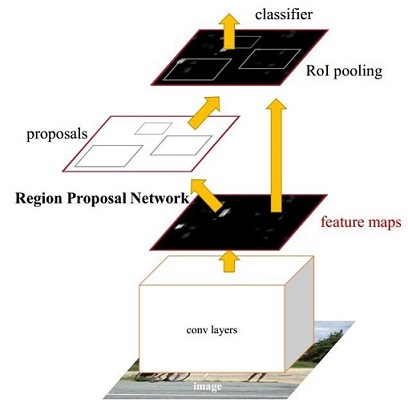
\includegraphics[width=0.5\textwidth]{Faster_R_CNN.png}
	\caption{Faster R-CNN基本结构}
	\label{Faster_R_CNN}
\end{figure}

如图\ref{Faster_R_CNN},Faster R-CNN可以根据功能的不同将模型分为四个模块:卷积层、区域候选网络(RPN)、兴趣区域池化(RoI Pooling)、分类器。卷积层使用CNN及其变型提取图像特征,生成的特征图被共享用于后续RPN层和全连接层,这种对图像的处理方式不同于R-CNN和Fast R-CNN。后两者都是先从原始图像中提取候选区域,再分别对候选区域提取特征。RPN网络用于预测候选区域,该网络在CNN输出的图像特征上滑动,在每个空间区域,网络都会预测类别得分,兴趣区域池化层结合图像的特征图和候选区域,得到区域特征图,再使用全连接层和分类器,预测每个区域的类别,同时利用候选框回归得到对象的检测框。

在本文中,我们使用联合在ImagNet\citing{russakovsky2015imagenet}上预训练的ResNet-101和在Visual Genome\citing{krishna2017visual}上预训练Faster R-CNN提取图像特征。给定图像$I$,我们从图像中提取$m$个大小不固定的图像特征,$X=\{x_1, x_2, ..., x_m\}, x_i \in \mathbb{R}^D$,每一个图像特征编码一个图像区域。每个图像区域的特征图维度为2048。对卷积层输出的特征图,我们使用非极大抑制(non-maximum suppression)和单元重合(IoU)阈值筛选出排名靠前的候选区域,通过设定一个目标检测概率的阈值,我们获得一个动态的被检测对象的数量$m \in [10,100]$,并且使用零填充使得$m=100$。对于每个所选区域$i$,$x_i$被定义为该区域的特征图的均值池化结果,并将$m$个区域的$x_i$拼接成为最终的图像特征。因此,每一张输入的图像将会被转化为一个$100\times 2048$的图像特征,供后续的注意力模块使用。

\section{基于ELMo的文本特征化}

如表\ref{model_compar}所示,以往的视觉问答模型的文本特征化都是通过对语料库的学习得到静态的词向量,即每个单词对应一个确定的实数向量,这种固定向量在处理词汇的多义性上表现不佳。无论是中文词语还是英文单词都广泛得存在一词多义的现象,即同一个词在不同的语境下含义发生变化,例如,在中文中,“他正在算账”和“下回找你算账”中的“算账”由于文化演化而产生了更复杂的引申义,又如英文中的“where is the bank?”和“It is the bank of the river”中的“bank”在第一句中译为“银行”而第二句中译为“河畔”。为解决一词多义的问题,研究者提出了动态词向量,ELMo和BERT便是其中的代表。ELMo在多个NLP任务中均提高了模型的准确率,因此本文将引入ELMo模型处理视觉问答任务中的文本,并在后续的处理中结合类似于BERT的注意力机制。

ELMo模型是一种能感知上下文的词向量生成模型,其模型深度能够有效建模词语复杂的语义和语法,能根据词语的上下文生成动态向量,进而为解决一词多义和一词多用提供了可能。ELMo采用了两个阶段获得词向量,第一个阶段是用大量的文本语料训练一个深度双向语言模型(biLSTM);第二个阶段从预训练网络中提取对应单词的网络各层的内部状态(internal state),并通过函数转化为词向量。ELMo模型的结构如图\ref{elmo}。
\begin{figure}[H]
	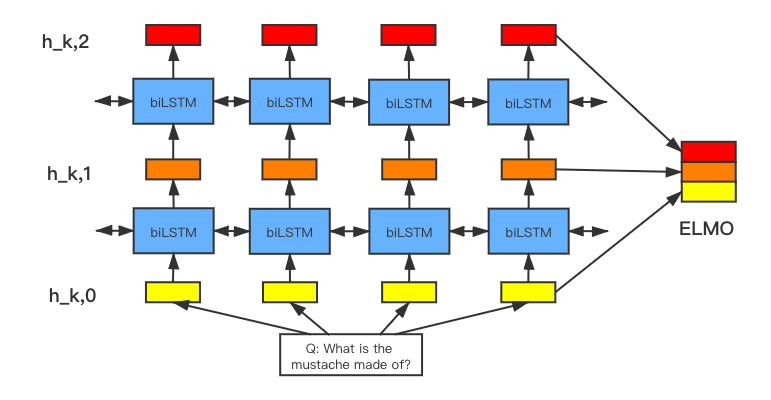
\includegraphics[width=0.8\textwidth]{elmo.png}
	\caption{ELMo模型架构}
	\label{elmo}
\end{figure}

语言模型是对语句的概率分布的建模。语言模型分为前向和后向,前向是指已知上文的词语,推理下一个词语的方式,而后向则是已知后文的内容,求解上一个词语的方式。对于一个具有N个单词的句子$S=(t_1, t_2, ..., t_N)$而言,前向语言模型就是求解以下公式的最大值:
\begin{equation}
p(t_1, t_2, ..., t_N)=\prod_{k=1}^N p(t_k|t_1,t_2,...,t_{k-1})
\end{equation}
其中$p(t_1, t_2, ..., t_N)$为序列的联合概率,
$p(t_k|t_1, t_2,..., t_{k-1})$表示已知$t_k$的上文$(t_1, t_2, ..., t_{k-1})$的条件下,求解$t_k$的条件概率。对应的后向语言模型的公式为
\begin{equation}
p(t_1, t_2, ..., t_N)=\prod_{k=1}^N p(t_k|t_{k+1},t_{k+2},...,t_N)
\end{equation}

ELMo使用双向LSTM(biLSTM)模型作为语言模型的基础。首先将“上下文无关的”初始词向量$y{_k^{LM}}$输入L层的前向LSTM。在位置k上,LSTM将输出一个“上下文相关”的词表征$\vec{h}_{k,j}^{LM,j}$,其中$j = 1, ..., L$。最后一层的LSTM输出$\vec{h}_{k,j}^{LM,L}$通过一个softmax层预测下一个词语的初始词向量$y{_{k+1}^{LM}}$。后向LSTM类似于前向LSTM有L层并且在k位置上得到一个词表征$\overleftarrow{h}_{k,j}^{LM}$。最后通过最大似然的方式训练双向LSTM模型,公式如下:
\begin{equation}
\sum_{k=1}^N(\log_p(t_k|t_1, t_2,..., t_{k-1};\Theta_x,\overrightarrow{\Theta_{LSTM}},\Theta_s) + \log_p(t_k|t_{k+1},t_{k+2},...,t_N;\Theta_x,\overleftarrow{\Theta_{LSTM}},\Theta_s)
)
\end{equation}

其中,$\Theta_x$和$\Theta_s$分别是训练阶段时的两个softmax层的参数,$\overrightarrow{\Theta_{LSTM}}$和$\overleftarrow{\Theta_{LSTM}}$是biLSTM的参数。

,完成预训练的模型对输入句子的每个单词输出三种Embedding:最底层是初始的词向量$y{_k^{LM}}$;前向LSTM输出的$\overrightarrow{h}_{k,j}^{LM}$;后向LSTM输出的$\overleftarrow{h}_{k,j}^{LM}$。ELMo将三种词向量串联,得到
\begin{equation}
R_k = 
[y_k^{LM}, \overrightarrow{h}_{k,j}^{LM}, \overleftarrow{h}_{k,j}^{LM} | j = 1, ..., L]
= [h_{k,j}^{LM} | j = 0, ..., L]
\end{equation}

其中$h_{k,0}^{LM}$是初始词向量,$h_{k,j}^{LM} = [\overrightarrow{h}_{k,j}^{LM}; \overleftarrow{h}_{k,j}^{LM}]$ 是每个biLSTM层输出的结果。

最后使用以下公式得到对应单词的具有”上下文信息“的词向量。
\begin{equation}
ELMo_k^{task} = E(R_k; \Theta^{task}) = \gamma^{task}\sum_{j=0}^L s_j^{task} h_{k,j}^{LM}
\end{equation}

其中是$s_j^{task}$任务相关训练得到的权重参数, $\gamma$是一个任务相关的scale参数。

在本文中,我们将句子最大长度裁剪为14个,并使用零填充的方式将不足14个词的句子补足为14,即$n=14$。并将每个单词转化为50维的初始词向量,即$y_k^{LM}\in \mathbb{R}^{50}$。假定双向语言模型的层数为$L = 2$,隐层节点数为$H_{dim}$,输出维度为$output_{dim} \in \mathbb{R}^d$,则$ELMo_k^{task} \in \mathbb{R}^{2d}$,输出的文本特征$Y \in \mathbb{R}^{n\times 2d}$。

\section{基于多头注意力机制的特征增强}
正如绪论中提到的,注意力机制的引入帮助神经网络提高了预测精度,并且减少了计算复杂度。视觉问答任务由于需要处理多模态的数据——图像和文本,比起仅需要处理单模态的数据的任务更需要进行高效的计算。同时,VQA任务输入的图像和问题文本具有高度的相关性,因此两种模态的数据之间的交互对于结果的准确性的提升也具有显著的影响。对于以上两个需求,我们在N-KBSN中使用了Transformer\citing{NIPS2017_7181}的多头注意力机制(Multi-head Attention, MA)实现图片的自注意力(V-SA)、问题文本的自注意力(Q-SA)、由问题引导的对图像的注意力(Guided Attention, GA)。

注意力机制本质上是找到一个方式对已有信息分配合适的权重,并以此提高输出的准确性。我们可以将注意力函数描述成映射查询(query)到一些键值对(key-value pair)并由此得到输出。假定查询矩阵$Q = \{q_1, q_2, ..., q_m\}$,其中查询向量$q_i \in \mathbb{R}^{1 \times d_q}$;key矩阵$K = \{k_1, k_2, ..., k_n\}$,其中$k_j\in \mathbb{R}^{1 \times d_k}$;value矩阵$V = \{v_1, v_2, ..., v_n\}$,其中value向量$v_i \in \mathbb{R}^{1 \times d_v}$,那么注意力特征可以通过对value矩阵的加权得到,权重可以通过查询矩阵和key矩阵得到:
\begin{equation}
Attention(Q, K, V) = score(Q, K)V
\end{equation}
其中$score(Q, K)$为计算权重的函数,有多种计算方式,本文使用Transformer中的缩放点乘法:
\begin{equation}
score(Q, K) = softmax(\frac{QK^T}{\sqrt{d_k}})
\end{equation}
其中$q_i$和$k_j$要求具有相同的维度。
因此可以得到:
\begin{equation}
Attention(Q, K, V) = softmax(\frac{QK^T}{\sqrt{d_k}})V
\end{equation}

为了进一步提高注意力特征的表达能力,引入多头注意力机制。多头注意力机制的实现过程是,将上式的$Q, K, V$输入到$h$个具有不同权重的线性层,得到$(Q_i, K_i, V_i), i = 1, 2, ..., h$,再分别计算得到$Attention(Q_i, K_i, V_i), i = 1, 2, ..., h$,最后将$h$个注意力特征拼接并通过一个线性层获得期望维度的注意力特征,如图\ref{ma}。多头注意力机制的公式为:
\begin{equation}
MA(Q, K, V) = [head_1, head_2, ..., head_h]W
\end{equation}
\begin{equation}
head_i = Attention(Q_i, K_i, V_i)
\end{equation}
其中$W$为线性层的权重。
\begin{figure}[H]
	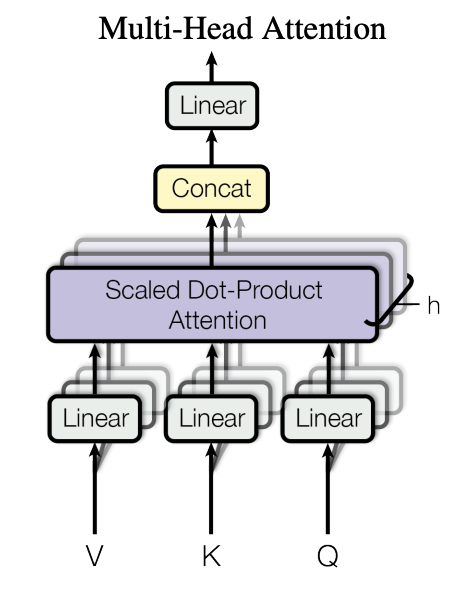
\includegraphics[width=0.5\textwidth]{ma.png}
	\caption{多头注意力的架构}
	\label{ma}
\end{figure}

基于以上多头注意力机制的思想,本文分别使用三种注意力特征:图片的自注意力(V-SA)、问题文本的自注意力(Q-SA)、由问题引导的对图像的注意力(GA)。假设文本词向量矩阵为$Y$,图像特征图为$X$,则在计算V-SA时,$Q = K = V = X$,即输出的图像特征为$SA=MA(X, X, X)$;在计算Q-SA时,$Q = K = V = Y$,即输出的文本特征为$SA=MA(Y, Y, Y)$;在计算引导注意力特征时,$Q = Y$为词向量矩阵,$K = V = X$为图像特征矩阵,并且词向量和图像特征向量具有相同的维度,即输出的由问题引导的图像特征为$GA=MA(Y, X, X)$。三种注意力组合的结构构成一个共同注意力模块(MCA),结构如图\ref{mca}。共同注意力模块以输入为原始的图像特征和文本特征,输出为经过注意力机制的图像和文本特征。
\begin{figure}[H]
	\includegraphics[width=0.3\textwidth]{mca.png}
	\caption{共同注意力模块结构}
	\label{mca}
\end{figure}

为了提高使用深度的注意力机制提取更高层次的特征,MCAN论文\citing{Yu_2019_CVPR}提出了Encoder-Decoder和Stacking两种级联MCA层的方式,如图\ref{mca_stacking}。其中,Stacking将上一层的输出直接作为下一层的输入,Encoder-Decoder将最后一层的问题自注意力特征作为每一层图像的查询矩阵。
\begin{figure}[H]
	\includegraphics[width=0.5\textwidth]{mca_stacking.png}
	\caption{两种MCA层的级联方式}
	\label{mca_stacking}
\end{figure}

根据文章给出的两种级联方式在多个任务的表现情况\citing{Yu_2019_CVPR},在本文中,我们使用Encoder-Decoder的级联方式,假定$SA^1$,$SA^2$,...,$SA^L$表示不同层的自注意力,$GA^1$,$GA^2$,...,$GA^L$表示不同层的引导注意力,$X^{(k)}$和$Y^{(k)}$分别表示第k层输出的图像特征和文本特征。因此第k层Encoder-Decoder级联的注意力模块的公式为,
\begin{equation}
Y^{(k)} = SA^{(k)}(Y^{(k-1)})
\end{equation}
\begin{equation}
X^{(k)} = GA^{(k)}(Y^{(L)}, SA^{(k)}(X^{(k-1)}))
\end{equation}
其中图像特征$X^{(0)}=X$,$Y^{(0)}=Y$。

在获得经过多层注意力的图像特征$X^{(L)}=[x^{(L)}_1,...,x^{(L)}_m]\in\mathbb{R}^{m \times d}$和文本特征$Y^{(L)}=[y^{(L)}_1,...,y^{(L)}_n]\in\mathbb{R}^{n \times d}$,我们对所有分量权重求和,进一步得到最终的图像特征$x$和文本特征$y$。以图像特征为例,公式如下。
\begin{equation}
\alpha = softmax(MLP(X^{(L)}))
\end{equation}
\begin{equation}
x = \sum_{i=1}^m \alpha_i x_i^{(L)}
\end{equation}
其中$\alpha = [\alpha_1,...,\alpha_m]$是图像特征分量的权重。

$Y^{(L)}$的计算方式类似。我们使用一下公式融合两种特征。
\begin{equation}
z = LayerNorm(W_x^Tx + W_y^Ty)
\end{equation}
其中$W_x, W_y \in \mathbb{R}^{d \times d_z}$是线性映射矩阵,$d_z$是融合后的特征向量的维度。最后我们使用softmax函数计算融合特征在$N$个类别的答案,$N$为训练集中出现频率最高的答案。最后我们使用交叉熵更新模型参数。

\section{实验}
本节将构建一系列有不同网络结构或者参数设置的视觉问答模型,并使用通用的开放型问答数据集VQA2.0\citing{goyal2017making}训练和评估模型。实验的目的是为了对比动态词向量和静态词向量对结果准确率的影响,并通过大量实验找到超参数最优的N-KBSN模型。整体代码使用Python实现,以pytorch为机器学习平台,并使用带有32G内存和GPU的计算机训练模型。

\subsection{实验设置}
\textbf{数据集}

我们使用VQA2.0数据集训练模型,数据集被划分为train/val/test三个数据子集,它们分别包含8万图像+44.4万问答对、4万图像+21.4万问答对、8万图像+44.8万问答对。答案包含“是否”、“数量”和“其他”三种类型,图片均为从MS-COCO数据集中提取的真实场景。此外,根据同时存在于VQA2.0和Visual Genome中的图片,我们还使用了从Visual Genome中提取出49万个问答对,用于增强训练集。

\textbf{评估方式}

为了实现对复杂推理的训练和测试,VQA2.0数据集在问题设置上采用了人工的方式,每张图片都有3个人类提出的问题。答案全为开放式问题,开放式答案的评估方法也引入人工评估机制:对于同一个开放性问题由十个人分别作答,如果有三个及以上的被测者均提供了同一答案,该答案被视为正确答案。
因此文本使用正确率作为评价参数,包括总体正确率和子项正确率。子项正确率根据答案类型分为是否、计数和其他。

\textbf{固定模块的参数设置}

本节的实验目的是对比不同的词向量嵌入策略对于模型的准确率的影响,因此模型的其他部分因保持相同的参数设置。具体来说,对于图像特征提取模块,Faster R-CNN的候选图像区域数$m = 100$,单个图像区域的特征维度$x_i = 2048$,因此单张图像特征$X \in \mathbb{R}^{100 \times 2048}$。自注意力和引导注意力模块中使用的多头注意力隐层维度$d=512$,头数$h=8$,即每个头的隐层维度$d_h=d/h=64$,MCA层数$L=6$。我们从所有答案中筛选出出现次数大于8的单词或词组,构建得到大小为$N=3129$答案词典,即分类的类别数为3129。

激活函数使用ReLU。Adam优化器参数为$\beta_1=0.9$、$\beta_2=0.98$,学习率为$min(2.5te^{-5}, 1e^{-4})$,其中t为训练的epoch数,从第10代开始,每过两代学习率衰减为当前的1/5。批样本数$batch = 32$,训练代数$epoch=13$。

\textbf{静态词向量 vs. 动态词向量}

在固定模型的其他部分不变的情况下, 我们将使用不同的本文特征化方法,以评估动态和静态词向量对于结果准确率的影响。我们选取了静态词向量中具有代表性、并且被广泛应用的预训练的word2vec和Glove词向量,并且级联一个单层的LSTM网络,将其特征维度转换为512维,便于后续和图像特征的融合。其中word2vec词向量使用的是word2vec模型在包含1000亿个单词和词组的Google News上训练得到的词向量。word2vec词向量是由表示300万个单词和词组的300维向量组成。Glove词向量是从Wikipedia和Twitter等语料库中训练得到,包含200万个300维的向量。为了使用静态词向量,我们首先输入样本的问题文本裁剪为长度为14的单词序列,再使用查找表得到每个单词的静态向量。对于数据集中不存在预训练词向量的单词,我们将其词向量初始化为零向量。

不同于静态向量的配置方式,为获得动态词向量,我们将预训练的深度双向LSTM网络(biLSTM)嵌入到模型中,并通过训练得到Elmo词向量的权重参数和尺度参数。为了进一步探究最佳的Elmo参数,我们选用了三种不同参数的预训练ELMO模型,分别是$ELMO_s$/$ELMO_m$/$ELMO_l$,它们的参数量、LSTM的隐层大小、输出大小、$ELMo_k^{task}$大小见表\ref{ELMO_models}。如表所示,三种不同参数的Elmo模型主要差异在于模型深度和词向量的维度,理论上来说,更深的网络深度具有更大的容量,并且高维的词向量能包含更多的语义信息。我们同样将问题文本裁剪为14个单词序列,并将整个单词序列作为输入,通过两层的biLSTM网络,得到包含上下文语境的Elmo词向量。我们同样使用一个LSTM网络将Elmo词向量统一转化为512维,融合特征$z \in \mathbb{R}^{1024}$。
\begin{table}[H]
% \resizebox{0.8\textwidth}{!}{}
\centering
\caption{三种 ELMO 的参数配置}
\begin{tabular}{ccccc}
\toprule
\textbf{Model} & \textbf{Parameters (Millions)} & \textbf{LSTM Size} & \textbf{Output Size} & \textbf{ELMO Size}\\
\midrule
$ELMO_s$&  13.6& 1024&  128& 256\\
$ELMO_m$&  28.0& 2048&  256& 512\\
$ELMO_l$&  93.6& 4096&  512& 1024\\
\bottomrule
\end{tabular}
\label{ELMO_models}
\end{table}

几种词向量的统计信息如表\ref{embedding_compare}。其中,由于Elmo模型使用字符级别的编码,因此即使对于语料库中不存在的单词,仍然可以获得其初始词向量,进而得到其Elmo词向量,因此Elmo词向量的数量理论上无限。为了方便实验结果的分析,我们将配置了不同文本特征的模型分别表示为:$baseline(w2v)$, $baseline(glove)$, $N-KBSN(s)$, $N-KBSN(m)$, $N-KBSN(l)$。
\begin{table}[H]
% \resizebox{0.8\textwidth}{!}{}
\centering
\caption{word2vec, Glove, 三种elmo模型的统计信息}
\begin{tabular}{c|c|c|c}
\toprule
\textbf{名称} & \textbf{预训练语料库(大小)} & \textbf{词向量维度} & \textbf{词向量数量} \\
\midrule
word2vec&  Google News(1000亿单词)& 300&  300万\\
Glove&  Wikipedia 2014 + Gigaword 5(60亿单词)& 300&  40万\\
\midrule
$ELMO_s$&  \multirow{3}{*}{WMT 2011(8亿单词)}& 256& \multirow{3}{*}{/}\\
$ELMO_m$&  & 512&  \\
$ELMO_l$&  & 1024&  \\
\bottomrule
\end{tabular}
\label{embedding_compare}
\end{table}

\subsection{实验结果及分析}

\subsubsection{VQA实验结果分析}

在本次的实验中,我们将使用VQA2.0数据集训练和评估六个模型,分别是$baseline(random)$, $baseline(w2v)$, $baseline(glove)$, $N-KBSN(s)$, $N-KBSN(m)$, $N-KBSN(l)$。其中$baseline(random)$的词向量使用随机初始化,并级联LSTM网络。同时,在模型对比中,我们也加入往年在VQA挑战中取得优胜的模型,$2017-winner(glove)$和$2019-winner(glove)$。各个模型在val验证集上的实验结果如表\ref{5mresults}。
\begin{table}[H]
% \resizebox{0.8\textwidth}{!}{}
\centering
\caption{使用不同文本特征化的模型在val数据集的结果}
\begin{tabular}{c|cccc}
\toprule
模型 & 总体正确率 & 是否 & 计数 & 其他\\
\midrule
$baseline(random)$& 62.34 &  78.77 & 41.92 & 55.27\\
$2017-winner(glove)$ & 63.22 & 80.07 & 42.87 & 55.81\\
$baseline(w2v)$&  64.37 &  81.89 &  44.51 & 56.31\\
$baseline(glove)$&  66.73 & 84.56 &  49.52 & 57.72\\
$2019-winner(glove)$& 67.22 & 84.80 & 49.30 & 58.60\\
\midrule
$N-KBSN(s)$&  67.27& 84.76&  49.31& 58.73\\
$N-KBSN(m)$&  67.55& 85.03&  49.62& 59.01\\
$N-KBSN(l)$&  \textbf{67.72}& \textbf{85.22}&  \textbf{49.63}& \textbf{59.20}\\
\bottomrule
\end{tabular}
\label{5mresults}
\end{table}

如表所示,从答案类型单项的准确率方面看,所有模型的实验结果都表现为,是否>其他>计数,且任意两个单项的准确率差值在不同模型的结果中保持稳定,这说明这种单项的准确率差异与模型无关,来源于问题本身和数据集的特性,例如,答案为是否的样本的随机猜测的期望准确率为50\%,而计数类型的随机猜测准确率很低,两种答案类型本身的难度差异导致了是否类型的准确率始终远远高于计数类型。

前五个模型均使用静态词向量作为文本特征,$baseline(random)$由于使用随机初始化的文本特征,词向量能包含的语义和语法信息相较于预训练词向量更少,因此其各项准确率均为最低。$2017-winner(glove)$由于使用更为简单的注意力机制,因此准确率低于本文的baseline模型。对比$baseline(w2v)$和$baseline(glove)$的实验结果,我们可以看出,即使word2vec词向量的语料库接近20倍于glove词向量的语料库,基于glove的模型还是呈现出全面的领先,在其他部分相同的情况下。分析其原因,正如论文\cite{pennington2014glove}所说,glove词向量使用了共现矩阵,相较于word2vec只使用局部的上下文信息,引入了语料库的全局信息,提高了表征能力,因此,即使使用了更大的语料库训练得到的word2vec词向量表征能力依然差于glove。

最后三个模型是本文提出的N-KBSN模型,从结果可以看出,对比$baseline(glove)$,各项的准确率均有显著提升,这证明了动态词向量确实能一定程度的提高模型的文本表示能力,进而提高整体的结果准确率。而对比三种不同参数的elmo模型,我们发现,随着模型深度和特征维度的提高,整体的准确率并没有特别明显的提高。具体来说,$N-KBSN(l)$的elmo模型参数量是$N-KBSN(m)$的三倍多,但是准确率并无明显提升。我们选用$N-KBSN(l)$作为参考模型,供之后的基于知识库图嵌入的KBSN模型使用。

如表\ref{5mresults}所呈现出的结果,使用了Elmo动态向量的N-KBSN模型的实验结果全面优于使用Glove静态词向量的$baseline(glove)$。为了进一步探究其原因,我们以$N-KBSN(m)$和$baseline(glove)$作为实验模型,进行了定量分析和定性分析。

\subsubsection{定量分析}
为了定量分析$N-KBSN(m)$和$baseline(glove)$的差异,我们将VQA2.0的train随机采样,分别构成大小为原始大小10\%, 30\%, 50\%, 70\%, 90\%, 100\%的训练子集,并按照之前实验相同的参数配置,训练两个模型。两个模型在val验证集上的总体准确率如表\ref{subsetres}所示,图示见\ref{subsetres_fig}。
\begin{table}[H]
% \resizebox{0.8\textwidth}{!}{}
\centering
\caption{$N-KBSN(m)$和$baseline(glove)$在不同训练子集的实验结果统计}
\begin{tabular}{cccc}
\toprule
准确率 & $baseline(glove)$ & $N-KBSN(m)$ & 差值\\
\midrule
训练子集(10\%)&  54.65 & \textbf{55.03} & 0.38\\
训练子集(30\%)&  60.30& \textbf{60.81} & 0.51\\
训练子集(50\%)&  62.87& \textbf{63.40} & 0.53\\
训练子集(70\%)&  64.12& \textbf{64.72} & 0.60\\
训练子集(90\%)&  65.98& \textbf{66.69} & 0.71\\
训练子集(100\%)& 66.73 & \textbf{67.55} & 0.82\\
\bottomrule
\end{tabular}
\label{subsetres}
\end{table}
\begin{figure}[H]
	\includegraphics[width=0.8\textwidth]{subsetres_fig.png}
	\caption{$N-KBSN(m)$和$baseline(glove)$在不同训练子集的实验结果统计图}
	\label{subsetres_fig}
\end{figure}

根据上述图和表格可以看出,随着训练数据的增加,各自的准确率均单调上升,并且上升的速度逐渐趋于减小,使得准确率趋于稳定,这说明增大训练数据量能够帮助提升准确率,但是提升会趋于饱和。值得注意的是,仅仅使用10\%的训练数据,也能得到较好的准确率。

$N-KBSN(m)$的准确率始终高于$baseline(glove)$,这说明动态词向量的确能提升模型的准确率。随着数据量的增大,两个模型的准确率差值逐渐增大,我们认为这是因为动态词向量能有效表征多义词的表现,更大的训练数据意味着更有可能包含词语在不同语境的使用,静态词向量则无法有效处理这种情况。

\subsubsection{定性分析}
为了定性的分析$N-KBSN(m)$和$baseline(glove)$在验证集结果的差异,我们将两个模型在验证集的预测结果进行对比分析,以下使用$Res(elmo)$和$Res(glove)$分别代表其结果集。$Res(elmo)$和$Res(glove)$的大小均为验证集中问题的数量:214354,其中,两个模型给出不同答案的问题数为52990,约占总数的1/5。在给出的不同答案中,$Res(elmo)$答对且$Res(glove)$答错的占比为27.8\%,$Res(glove)$答对且$Res(elmo)$答错的占比为26.4\%,结果都错的比例为45.8\%,结果都对的比例为0\%,如表\ref{diff}。
\begin{table}[H]
% \resizebox{0.8\textwidth}{!}{}
\centering
\caption{$Res(elmo)$和$Res(glove)$在验证集的答案的差异}
\begin{tabular}{cc}
\toprule
不同答案的问题数(比例) & 52,990 (24.7\%)\\
仅$Res(elmo)$答对数(比例) & 14,711 (27.8\%)\\
仅$Res(glove)$答对数(比例) & 13,991 (26.4\%)\\
都答错数(比例)& 24288 (45.8\%)\\
都答对数(比例)& 0 (0\%) \\
\bottomrule
\end{tabular}
\label{diff}
\end{table}
从总体的答案差异看,$N-KBSN(m)$答对的数量略高于$baseline(glove)$,这也符合验证集上的整体结果的表现。

我们还从答案中,挑选了一些样本来定性分析$N-KBSN(m)$优于$baseline(glove)$的可能原因,如图\ref{res_examples}。图(a)$Res(elmo)$正确识别出“浴池窗帘”的颜色,而$Res(glove)$的答案则为”白色“,我们认为这是模型错误的识别了"shower"而不是"shower curtain"的颜色。在图(b)中类似,$Res(glove)$计数对象为"people"而$Res(elmo)$则能正确的计数"elderly people"词组。图(c)则体现了$Res(elmo)$能更好的识别长句中的词组而不仅仅是识别单词的能力。
\begin{figure}[H]
	\includegraphics[width=0.8\textwidth]{res_examples.png}
	\caption{验证集的样本示例}
	\label{res_examples}
\end{figure}

\subsubsection{和已有模型的比较}
如表\ref{5mresults}所示,$N-KBSN(l)$在验证集上表现最佳,该模型和$2017-winner(glove)$和$2019-winner(glove)$在Test-dev和Test-std测试集上的结果如表\ref{testres}。测试集上的结果显示,我们提出的$N-KBSN(l)$在各项指标上均优于其他两个模型,该结果和验证集上的结果表现一致,这证明了我们改进的文本特征化方式能够提高预测的准确率。
\begin{table}[H]
% \resizebox{0.8\textwidth}{!}{}
\centering
\caption{$N-KBSN(l)$模型和其他模型在测试集上的结果对比}
\begin{tabular}{c|cccc|c}
\toprule
\multirow{2}{*}{模型} & \multicolumn{4}{c}{Test-dev} & Test-std\\
& All & Y/N & Num & Other & All \\
\midrule
$2017-winner(glove)$ & 65.32 & 81.82 & 44.21 & 56.05 & 65.67\\
$2019-winner(glove)$ & 70.63 & 86.82 & 53.26 & 60.72 & 70.90\\
\midrule
$N-KBSN(l)$& \textbf{71.14} & \textbf{87.13} & \textbf{54.05} & \textbf{60.90} & \textbf{71.23} \\
\bottomrule
\end{tabular}
\label{testres}
\end{table}

\section{本章小结}
本章的主要内容是构建了一个基于动态词向量的联合嵌入模型(N-KBSN模型),并通过对比实验证明了动态词向量能够提高视觉问答模型的性能。

本章首先介绍了视觉问答挑战的发展情况,进一步解释了联合嵌入模型主流地位和优异表现的原因。通过对比已有代表性的联合嵌入模型,我们分析了其潜在的改进方向,从而提出了了一个基于动态词向量的联合嵌入模型——None KB-Specific Network(N-KBSN)模型。随后详细介绍了N-KBSN模型的关键部分:基于Faster R-CNN的图像特征化、基于ELMo的文本特征化和基于多头注意力机制的特征增强。

实验部分,我们使用通用的VQA2.0数据集训练和验证模型。为了探究动态词向量和静态词向量对实验结果的影响,我们固定其他模块不变,使用不同的本文特征化方法构建了多个模型。实验结果证明动态词向量的引入提高了整体结果的准确率,本文构建的N-KBSN实现了较高的预测准确率。随后,我们进一步对$N-KBSN(m)$和$baseline(glove)$进行了定性和定量分析,分析结果解释了基于动态词向量的模型整体优于静态模型的原因,也证明了引入动态词向量的有效性。




\chapter{基于知识库图嵌入的视觉问答模型}
\section{知识库概述}
人类智能体通过学习和实践不断获取知识与经验,并能将习得的知识存储在记忆系统中,面对相关问题时能准确、快速地调用相关的知识和经验,完成识别和推理过程,成功解决问题。人工智能系统的终极目标便是能像人类一般快速、准确地解决未知问题,甚至超越人类的物理极限,实现范围更广、更艰深的任务解决。人类在真实世界中的学习是不断将非结构化的信息重构为结构化的知识的过程,知识库(KB)是一种包含常识和描述真实世界的事实的知识集,在不同的应用情景中有不同的内部结构。

知识库最早被应用于人工智能中的专家系统\citing{akerkar2010knowledge},专家系统是一种建立在知识库基础上,使用推理方法完成复杂推理过程,最终实现与人类专家同水平的决策能力的计算机系统,被广泛应用于医学诊断、分子结构推理、自然语言理解等领域。专家系统面向的专家任务需要特定领域的知识,这也使得知识库成为专家系统的核心之一。针对不同领域的任务构建知识的表达方式是困难的,因为专家知识可能是不精确的,同时要从知识库中获取答案的过程依赖于人工的制定复杂的规则,知识库精度和人力成本等因素制约了专家系统在更多领域的应用。

知识库也被应用于在自然语言处理的任务,例如机器翻译和文本问答。知识库中的本体包含某个领域中的各种概念和概念间的关系,本体在机器翻译中可作为知识源\citing{nirenburg1994machine}。语言学中的多义词在不同的语境中被解释为不同的含义,人类能根据上下文语境的不同选择出最恰当的词语,但对于机器翻译系统便是一大难题。当机器翻译系统能够获得足够多的本体作为知识源时,能较好地解决多义词的解释问题,从而得到更加准确的翻译结果\citing{knight1993building}。

文本问答系统在早期作为专家系统的交互界面,在之后的发展中逐渐独立出来成为自然语言处理的一个分支,文本问答系统根据给出的文本问题,从文本知识库中提取答案,此时的文本知识库往往是文本组成的文档,还未使用资源描述框架(RDF)的结构化数据。大多数文本问答系统都采用相对标准的结构:根据问题文本建立查询、利用信息提取方法(IR)确定可能包含答案的文章位置、进一步确定答案所在的片段,这种架构下不使用任何与答案相关的额外知识\citing{hermjakob2000knowledge}。Hermjakob等人提出了将手写规则和概念本体相结合的问答系统——Webclopedia\citing{hermjakob2000knowledge}。Webclopedia由对输入问题进行句法和语义的解析的问题解析模块、用于文档查询的查询模块、用于获得与答案相关的文档的信息提取模块、片段解析模块、答案匹配模块和答案生成模块构成。系统在多个模块中使用了知识库提高精确度,在问题解析过程中使用了语言知识库——由30000个节点的概念层级、140个问题/答案类型和词库组成,帮助系统确定问题的句法结构;在查询模块中使用了WordNet\citing{miller1995wordnet}扩展与问题关键词关联的信息;在答案匹配模块中也使用了常识和事实知识库,系统的架构如图\ref{Webclopedia}。
\begin{figure}[H]
	\centering
	\includegraphics[width=0.8\textwidth]{Webclopedia.png}
	\caption{Webclopedia系统架构}
	\label{Webclopedia}
\end{figure}

应用信息提取技术(IR)的问答系统有一个非常明显的缺点——只能根据问题确定答案相关的文章或者段落,不能给出更为直接的答案。为解决这种缺陷,研究人员探索了更多的方法。

Burke等人一改通常的从文章中提取答案的方式,先将被频繁问到的问题(FAQ)以“问题-答案”对的形式存储为知识库,再从新问题中寻找与知识库匹配程度最高的“问题-答案”对,进而获得答案\citing{burke1997question}。在此方法中最核心的步骤是对新旧问题之间的匹配,为了使匹配的问题之间的语义相似度最大,系统还使用了WordNet\citing{miller1995wordnet}的语义知识,WordNet能提供词语和其同义词集合、同义词集合之间的关系,因此能避免一些匹配过程中的歧义错误,提高匹配的准确度。这里以“匹配”为核心思想的算法最大的障碍是常见问题集的容量、深度和广度问题,因此通常对于范围较小的场景而言,才能实现较好的匹配准确度。Rinaldi等人提出一个专门针对技术领域的基于知识的问答系统ExtrAns\citing{rinaldi2002towards}。ExtrAns以技术手册为知识库,将问题文本和知识库都转化为一种称为“最小逻辑形式”(MLF)的语义表达,并通过逻辑证明提取出答案。

随着资源描述框架(RDF)在构建知识库的兴起,知识库也由原来的文档形式转化为冗余更小、可扩展性更强、易用性更强的结构化数据库。面对由于互联网技术的普及带来的海量网页、文章、超文本、图片等多种模态的资源,研究者们对信息的整合进行了探索\citing{smith1981multibase,wiederhold1993intelligent,subrahmanian1994amalgamating,embley1998ontology,alani2003automatic},语义网和相关技术的出现促进了大尺度知识库的发展,出现了DBpedia\citing{auer2007dbpedia}、OpenIE\citing{banko2007open}、Yago\citing{suchanek2007yago}、Freebase\citing{bollacker2008freebase}、Wikidata\citing{vrandevcic2014wikidata}等多种含有常识和特定领域知识的知识库,这些配置灵活、结构统一且语义丰富的外源知识库也促进了基于知识库的视觉问答方法的兴起。

\begin{comment}
\section{常见的知识库}
知识表达是人工智能中历史较为悠久的领域,并且大量的知识表达模型被提出,从最早的“框架和脚本”(frame and script)\citing{minsky1974framework,schank2013scripts}到后来的逻辑表达方式、资源描述框架(RDF)和网络本体语言(OWL)。随着互联网技术的普及,海量的网页、文章、超文本、图片等多种模态的资源被创造,如何将这些海量松散的多模数据重组为结构化的数据成为计算机科学的重要任务之一,大量的研究对信息的整合进行了探索\citing{smith1981multibase,wiederhold1993intelligent,subrahmanian1994amalgamating,embley1998ontology,alani2003automatic},语义网和相关技术的出现促进了大尺度知识库的发展,出现了DBpedia\citing{auer2007dbpedia}、OpenIE\citing{banko2007open}、Yago\citing{suchanek2007yago}、Freebase\citing{bollacker2008freebase}、Wikidata\citing{vrandevcic2014wikidata}等多种含有常识和特定领域知识的知识库。

除了知识库以外还有一种常用的存储数据的方式——数据库。数据库通常被组织成表格的方式,表内使用数值或者字符的方式表示数据,首行罗列出不同的属性,其余行则代表存储的数据。数据库中的表与表之间存在的指针代表表之间的联系。不同于数据库,知识库不以表为组织形式,而是由大量形式为(主语,谓语,宾语)的三元组构成的图结构,这样的三元组以资源描述框架(RDF)为模型基础\citing{lassila1997resource},能够方便的通过查询语句获得信息。“主语”和“宾语”表示知识库中的实体,“谓语”代表两者之间的关系。例如,将“猫种类属于哺乳类”转化的三元组形式为(猫,种类属于,哺乳类),“猫”是主语,“种类属于”是谓语,“哺乳类”是宾语。数据库与知识库的结构对比如图\ref{db-kb}。
\begin{figure}[H]
	\centering
	\subfigure[数据库的表结构]{
		\includegraphics[width=0.5\textwidth]{database.jpg}}
	\subfigure[知识库的由三元组构成的图结构]{
		\includegraphics[width=0.7\textwidth]{kb.png}}
	\caption{数据库与知识库不同的数据组织形式}
	\label{db-kb}
\end{figure}

知识库具有高通用性、高可读性的特征。通过资源描述框架(RDF)能将所有现实中可描述的事物和事物间的关系组织到知识库中,这种通用性特征能够极大地提高了自动化系统存储、交换和使用信息;三元组的结构来源于语言学中“主谓宾”的基本语句构成方式,这既符合人类的认知方式,也是一种简单的数据组织形式,因此高可读性即使针对人类可读也是针对机器可读。正是因为知识库是建立在真实世界事实的描述之上,因此它能成为复杂决策和推理的基石,从人类推理过程看,知识库便是复杂推理的“起点”。
\end{comment}

\textbf{Yago}
知识库通常由人工和自动化提取两种方式构建得到,对比这两种不同构建方式,自动化提取的知识库往往质量较低,容易包含错误信息,而人工构建的知识库能满足较高的精度要求,但由于人工构建的成本较高,因此此类知识库有数据容量受限、构建周期长、内容老化快等缺陷。

Suchanek等人结合Wikipedia文章的广博性和WordNet优秀的语义分类,提出了自动化生成本体的知识库YAGO\citing{suchanek2007yago}。Wikipedia的文章对某个话题或概念进行详细的多角度说明,同时大多数文章都归属于一个或者多个类别,类别页面既包含了大量实体和概念,可以作为知识库中的本体,同时类别页面也隐含着概念之间的平行关系和所属关系,这能提供一定的结构关系。YAGO利用Wikipedia目录页面提取出其中的实体和实体之间的关系,同时结合WordNet中概念的清晰层次关系,实现了97\%的准确率。初始版本中涉及90万个实体和500万个实体之间的关系。

YAGO被设计为可扩展的知识库,能够结合特定领域的知识源或是从网络上提取得到的信息构建领域相关的知识库,因此之后的研究者也在此基础上进行了多种的扩展。YAGO2在YAGO基础上引入GeoNames——包含超过700万个地点信息,在“实体-关联”的表示方法中加入了时间和空间维度,不仅能丰富事实的准确性,还能反应出实体在时空层面的变化\citing{hoffart2013yago2}。YAGO3构建了一个多语言的知识库\citing{mahdisoltani2013yago3}。

\textbf{DBpedia}
Wikipedia是由非盈利组织维基媒体基金会(Wikimedia Foundation)构建的世界上最大的多语言的开放性网络百科全书,其通过文章的形式对词条进行多方面的介绍,文章中包含大量的结构化信息,例如文字、信息框模板、分类信息、图片、地理坐标信息、超链接等,这些多模态的信息能丰富知识的多样性,并且建立知识的关联。但作为网络应用,Wikipedia的搜索能力和其他网络应用一样,只能满足关键词的搜索,这种状况大大的降低了知识之间的关联和价值,同时因为其作为大规模协同性内容编辑平台,文章内容也难以避免的出现数据矛盾、不一致的分类和错误。

Auer等人为了充分挖掘Wikipedia中已有的人类知识,并构建知识结构,提出了DBpedia知识库\citing{auer2007dbpedia}。Wikipedia为实现统一的文章风格,因此在文章编辑中镶嵌了一些信息框模板,如图\ref{dbpedia}。
\begin{figure}[h]
	\centering
	\includegraphics[width=0.8\textwidth]{dbpedia.png}
	\caption{Wikipedia的信息框模板和加载效果}
	\label{dbpedia}
\end{figure}
DBpedia利用信息框提取算法检测信息框模板,并且提取出关键的信息,再将信息转化为资源描述框架(RDF)的三元组结构,从而将Wikipedia的文章内容转化为机器可读的结构化信息。最初版本的DBpedia知识库包含关于195万实体的信息,实体内容包括人物、地点、音乐专辑和电影,除了实体外还包含65.7万个图片链接、160万个外部网页链接、18万个其他资源描述框架(RDF)数据库、20.7万个Wikipedia目录和7.5万个YAGO类别\citing{suchanek2007yago}。随着开放社区的数据丰富,2016年推出的版本中已经包含6600万实体,实体的类型扩充了视频、游戏、组织、物种和疾病\citing{wikipedia2016}。资源描述框架的三元组数据量也从1亿增长到130亿之多。

为了增强DBpedia的数据易用性,Auer等人提供了三种数据获取方式:链接数据、SPARQL协议和可下载的RDF文件。链接数据通过HTTP协议获取发布与互联网上的RDF数据,提供给语义网络浏览器、语义网路爬虫和语义网络查询客户端访问\citing{timlinked}。SPARQL是专门针对资源描述框架的查询语言,通过SPARQL终端向\url{http://dbpedia.org/sparql}发送查询指令,DBpedia知识库会返回相应的查询结果。可下载的RDF文件包含序列化的RDF三元组数据,DBpedia将整个数据库按照数据的类型分为众多子数据集,例如,文章目录集、目录标签集、地理坐标集、图像集等。

知识库的内容多样性、易用性和大体量为DBpedia应用提供了良好的基础设施,因此一些自然语言问答和交互的应用都选择建立在DBpedia丰富的知识之上。NLI-GO DBpedia是一个针对通用自然语言交互的应用程序,程序可以接受自然语言问题,并通过SPARQL查询DBpedia知识库,给出答案,实际上这就是基于DBpedia的文本问答系统\citing{nli-go},类似的还有款基于DBpedia的聊天机器人——DBpedia Chatbot。许多基于知识库的视觉问答研究也选择了数据更加准确的DBpedia\citing{wang2015explicit,wang2017fvqa,wu2016ask}。

\textbf{OpenIE}
应用于构建知识库的信息提取技术(IR)往往需要人为构建大量手写规则,并选择合适的语料库,当已有的提取模型面对全新领域的语料库时,需要重新编写提取规则或者标注数据,这种系统在面对快速迭代和具有丰富多样性的互联网数据时,便会遇到自动化程度低、语料库异质性和效率问题。

为了节省信息提取过程的自动化程度,并能大范围应用于不同领域,Banko等人提出了一种能自主学习不同语料库的信息提取模型——开放信息提取技术(Open IE)\citing{banko2007open}。Open IE以语料库为输入,通过内部算法对语料库中的语句进行一次遍历,最终提取出语句中蕴含的(实体,关系,实体)三元组数据,在整个过程中不需要人工参与,因此可以应用于不同领域知识库的构建。

Banko等人还提出了一种应用高扩展性Open IE模型的系统TEXTRUNNER。TEXTRUNNER由自监督学习器、单通道提取器、基于冗余的评估器三个主要模块构成。自监督学习器以小的语料样本作为训练集,首先使用语句解析器从样本中粗略地提取出(实体,关系,实体)的三元组数据,再对提取出的内容进行标注,标注为“可信”和“不可信”两种标签,将带有标签的数据作为朴素贝叶斯分类器的训练样本。提取器遍历整个语料库,提取出所有可能的三元组数据。对于同一个句子,提取器能生成一个或多个三元组数据,这些数据将被送入学习器训练得到的分类器中,保留所有分在“可信”类别的数据。在得到所有提取出的知识后,评估器融合相同的数据,计算不同的数据的数量。基于以上统计,评估器对每一个三元组数据分配一个用于判断知识正确性的概率值,其中的假设是,如果从多个的语句中提取出相同的知识,那么该知识拥有较高的可信度。

在实验阶段,TEXTRUNNER从包含1.3亿个句子的900万个网页中提取出6000万个三元组数据,平均每个句子提取出2.2个关系数据。通过数据过滤、随机抽取、人工判定等方式,作者对提取数据的完整性和正确性进行了概率评估,过滤后的数据包含1130万个三元组数据,其中780万的数据被评估为“格式正确”且概率标签在0.8以上,80.4\%“格式正确”的数据通过人工评估被认定为正确的,从实体间的关系看,“格式正确”的数据中反映抽象事实的占86\%,其中77.2\%是正确的;反映具体事实的占14\%,其中88.1\%是正确的,如图所示\ref{textrunner}。
\begin{figure}[H]
	\centering
	\includegraphics[width=0.5\textwidth]{textrunner.png}
	\caption{TEXTRUNNER在实验环境下知识提取的正确率}
	\label{textrunner}
\end{figure}

Wu等人在TEXTRUNNER的基础上提出了WOE开放信息提取系统\citing{wu2010open}。WOE改进了自监督学习方式用于构建提取器,TEXTRUNNER在提取过程中使用解析器直接从语料库中提取(实体,关系,实体)的三元组数据,而WOE则先从Wikipedia的信息框中提取“属性-值”对,再使用匹配器从文章中找到包含文章主语和“属性-值”对的句子作为语料库中的训练数据。随后测试了两种解析方法的提取器:WOE-parse和WOE-pos,WOE-pos使用和TEXTRUNNER类似的解析方法,根据简单的词性标签,从语料库中的句子解析出(实体,关系,实体)的数据,WOE-parse则选择更复杂的依赖解析树,希望能再复杂长句的解析中得到更好的精确度。

开放信息提取系统会对每个输出的三元组数据给定一个置信度,如果给定一个置信度的下限,高置信度的数据被保留,低置信度的数据被过滤,此时可以通过精确度和召回率测试系统的性能。精确度是指保留的数据中正确的数据所占比例,能反映整体精确度的平均水平。召回率是指保留的数据中正确的数据占所有正确数据的比例,能反映正确的数据在不同置信度的分布情况。

实验分析显示,因为使用了更友好的训练数据,WOE-pos在精确度上更优于TEXTRUNNER,而WOE-parse在解析树的帮助下实现了最好的性能,特别是在召回率上。

Fader等人在分析TEXTRUNNER和WOE的结果之后发现,不连贯提取和无信息提取两种错误频繁出现。不连贯提取是指被提取的关系语句由多词组成,但语义不连贯而无意义。无信息提取是指提取内容忽略了句子的关键信息,例如,“父亲对母亲做出承诺”,系统返回无信息的(父亲,做出,承诺)而不是(父亲,做出承诺对,母亲)。以上的两种错误都是由系统不能提取出具有完整句法结构的关系语句造成的,Fader等人在Open IE系统中引入了一定的句法限制,提出了REVERB开放信息提取系统\citing{fader2011identifying}。30\%的REVERB提取数据的概率标签在0.8或更高,相较起TEXTRUNNER的0.13\%,在精确度上实现了越阶式的增长,不连贯提取和无信息提取的错误率也大幅减少。

\textbf{Freebase}
Bollacker等人试图结合一般数据库的扩展和Wikipedia等百科全书的多样性,提出了Freebase数据库\citing{bollacker2008freebase}。Freebase和其他常用的知识库相同,使用资源描述框架的三元组形式结构化真实世界的知识,但同时继承了网络百科全书的开放和协同的思想,所有的内容创造和维护都由社区成员协作完成。Freebase存储的元组数据超过1亿2500万条,超过4000种类型和7000种属性,允许使用查询语言通过HTTP协议获取数据。

2014年,Google宣布关停Freebase并将数据迁移至Wikidata。

\textbf{Wikidata}
Wikidata是为了更高效地开放使用和管理Wikipedia文章中数据而提出的协同知识库\citing{vrandevcic2014wikidata}。由于Wikidata的出发点是希望通过大规模协同的方式构建知识库,因此Wikidata的数据具有开放性、多版本共存、多语言、易用性和持续更新的特性。Wikidata向所有用户提供数据扩展和编辑的权限;Wikidata为保证模糊数据的存疑性,相互之间有冲突的数据被同时展示;考虑到数字、日期、坐标等语言无关的数据内容,Wikidata与Wikipedia相同设计为多语言版本;Wikidata数据被组织成Json、RDF的形式发布于网络,通过网络服务能够轻松获取数据;社区成员的持续更新能保持Wikidata的时效性。

Wikidata数据的基本单元被称为项目(Item),每个项目包含名称标签、“Q+数字“的项目编码、描述、别名、和声明。声明中包含一系列属性和相应的值,用于详细描述项目的特点,项目页面如图\ref{wiki-item}。
\begin{figure}[H]
	\centering
	\includegraphics[width=0.8\textwidth]{wiki-item.png}
	\caption{wikidata项目页面}
	\label{wiki-item}
\end{figure}
项目之间通过有向无环图的方式构成,节点代表项目,有向线段代表项目之间的关系,如图\ref{wiki-dag}。截止到2018年,Wikidata已拥有超过5000万个项目。
\begin{figure}[H]
	\centering
	\includegraphics[width=0.8\textwidth]{wiki-dag.png}
	\caption{wikidata项目之间的有向无环图结构}
	\label{wiki-dag}
\end{figure}

Wikidata于2012年提出,相较起以往的知识库,开放性更强,限制也更少。对比YAGO和DBpedia,Wikidata不是从Wikipedia的目录或者信息框中提取信息,相反Wikidata被社区成员独立构建,并为Wikipedia作为知识源,数据被链接到Wikipedia文章中。对比Freebase将对象按类型划分的方式,Wikidata支持对所有对象赋予任意属性。

\section{KBSN模型}
使用RDF的数据表达方式,实体和实体之间通过属性建立了联系,这些有丰富语义的实体之间相互联系,构成了知识库。通过可视化的方式,实体作为节点,属性或者实体关系为边,知识库可以以图的形式呈现,因此知识库也被称为知识图谱。

正如绪论中提到的,知识库因其丰富的知识存储量、多样化的知识内容、复杂的知识关联、结构化的数据存储方式,可以作为问答系统或者其他信息检索任务的重要基础。目前使用知识图谱的主流方式是通过SPARQL等结构化查询语言对知识库中的内容进行精准的检索和提取,这种方式人为地建立查询规则、设计相应的知识库存储。

在基于知识库的视觉问答模型中,知识库的使用方式大致分为两种。一种方式为知识库查询类,依照主流的知识库查询的思路,模型提取图片的实体、将实体映射到知识库、转化自然语言为查询语句、查询知识库\citing{wang2015explicit, wang2017fvqa}。这些模型依靠精准的查询语句,对于预先设定好的模板问题能实现优于基线模型的准确率,然而却面临着问题模板设计成本高、数据集难构建、模型泛化能力差等缺点。

另一种方式为联合嵌入类,这种方式不用设计复杂的查询语句,而是将知识库的文本信息转化为额外的特征向量,并联合图像特征和问题特征一起训练。这种方式能省去问题模板和查询语句设计的人工成本,并将模型在更大规模的开放性数据集进行训练。然而,此前的模型却仅仅使用知识库中单个节点的文本信息,例如论文\citing{wu2016ask}根据从图像中预测的属性生成DBpedia查询,得到相关属性的“comment”本文内容,再将这种成段的文本信息转换为固定的特征向量,作为由知识库提供的额外特征与其他两种模态的特征融合。在这种方式中,模型虽然引入了额外的特征,试图提高表征能力,但是这种额外特征仅仅局限于单个节点,因此必然损失了节点互联形成的结构关系,而这种结构关系正是知识库的核心——通过多种关系连接而组织起来的具有丰富语义表征能力的实体网络。

为了利用知识库中关联数据的结构信息,我们在N-KBSN模型的基础上,引入使用图嵌入表示的知识库,提出了KBSN模型。KBSN模型使用了N-KBSN模型的问题文本和图像特征提取模块、自注意力和引导注意力模块,而在特征融合时引入了知识库的图嵌入。

知识库的图嵌入是KBSN模型有别于其他基于知识库的视觉问答模型的创新之处,其背后的思路为:先从图像和问题文本中识别出核心概念,将核心概念映射为知识库中的核心实体,通过剔除核心实体外无关的实体和链接形成以核心实体为中心的子图,再将各个子图转换为图嵌入,最后子图嵌入融合为图嵌入,以此作为额外特征。

按照以上的思路,知识库的图嵌入由子图提取模块和子图嵌入模块两个主要部分组成。子图提取模块的作用是完成从图像和问题文本到知识库的映射。具体来说,子图提取模块包含“图像-知识库映射”和“文本-知识库映射”。“图像-知识库映射”使用Faster R-CNN预测得到图像中包含的物体,再使用SPARQL查询知识库,得到图像相关的核心实体,“文本-知识库映射”使用DBpedia Spotlight\citing{isem2013daiber}模型识别、整合问题文本,得到问题相关的核心实体。需要指出的是,在此,我们不是使用完整的DBpedia知识库,而是根据问答这种任务类型的特点,挑选出特定的数据子集构成实验知识库。

子图嵌入模块是将提取得到的子图映射为图嵌入。具体来说,我们首先使用实验知识库训练TransE模型,得到实验知识库的嵌入表示。然而将子图提取模块输出的子图的节点和边都映射为向量,最后经过图神经网络获得子图的嵌入表示。

最后将子图的嵌入表示、图像特征、文本特征三者融合,分类得到答案,KBSN的基础架构如图\ref{KBSN}。
\begin{figure}[H]
	\centering
	\includegraphics[width=0.8\textwidth]{KBSN.png}
	\caption{KBSN的基础架构}
	\label{KBSN}
\end{figure}

\subsection{知识库子图提取}
对于基于知识库的视觉问答任务而言,准确的实现自然语言和图像中涉及的实体到知识库实体的映射是至关重要的,一方面能够大大地减少知识库中无关信息的噪声干扰,提高精确度,另一方面准确的映射能够极大的减少计算冗余,提高运行速度。

在知识库子图提取的准确性和计算效率综合的考量下,我们首先以DBpedia为基础,收集了部分子数据集组成实验知识库,再使用在N-KBSN模型中相同的Faster R-CNN从图像中识别出关键实体,再设计SPARQL查询语句从实验知识库中提取出图像相关的子图。另一方面,对于问题文本中的核心实体,我们直接使用DBpedia Spotlight完成从文本到DBpedia节点的映射,进而提取出问题相关的子图。

需要注意的是,针对图像的物体识别是使用的N-KBSN的Faster R-CNN,但是在N-KBSN中,是将所有区域的图像特征融合作为图像特征,而此处则加上分类层,使用softmax预测并输出各个区域的类别信息。由于使用的Faster R-CNN已经在之前的章节详细介绍了,本节将省略面向图像的子图提取,重点介绍面向文本的子图提取。

\subsubsection{知识库收集和分析}
在本文中,因为DBpedia丰富的实体及其属性,并且相对规范和统一的数据内容,我们使用DBpedia作为提供额外特征的知识库。然而由于DBpedia从众包的wikipedia提取得到,因此知识库中除去我们关心的和实体语义高度相关的属性外,还保留着一些基于语义网思想的属性,例如用于连接其他知识库实体的外链、参考引用的外链、主页地址、图片链接、未经处理的infobox属性等,除此之外,完整数据集中还包含包括英语在内的多语言版本,而以上这些信息对于回答开放性问题帮助很小,因此在本文的研究中,我们甄选了DBpedia数据集中“语义高度相关”的子数据集构成实验知识库,具体的数据集和其简要描述如表\ref{dbpeidaList},知识库的参数统计如表\ref{dbpediaPara}。
\begin{table}[H]
% \resizebox{0.8\textwidth}{!}{}
\centering
\caption{实验知识库包含的DBpedia数据子集及其描述}
\begin{tabular*}{0.9\textwidth}{lc}
\toprule
\textbf{DBpedia数据集} & \textbf{描述}\\
\midrule
instance\_types\_en & 连接实体及其类型 \\
labels\_en & 实体标签 \\
mappingbased\_literals\_en & 连接object为literal的高质量的谓语 \\
mappingbased\_objects\_en & 连接object为对象的高质量的谓语 \\
persondata\_en & 和person相关的信息,例如出生日期等 \\
\bottomrule
\end{tabular*}
\label{dbpeidaList}
\end{table}
\begin{table}[H]
% \resizebox{0.8\textwidth}{!}{}
\centering
\caption{实验知识库的参数统计}
\begin{tabular}{lc}
\toprule
\textbf{统计参数} & \textbf{数量}\\
\midrule
三元组 &  59,998,758\\
类 &  426\\
实体 & 5,377,081 \\
主语 & 14,556,042 \\
属性 & 1,377 \\
宾语 & 19,495,719 \\
\bottomrule
\end{tabular}
\label{dbpediaPara}
\end{table}

正如表\ref{dbpeidaList}所示,实验知识库只包含了英语版本的知识库,但值得注意的是,本文提出的模型结构同样适用于其他语言类型,扩展到多语言的应用只需要将数据集和知识库替换为指定语言版本即可。实验知识库包含完整的类别信息、完整的实体标签和高质量的属性信息,足够应对绝大部分的常规问题,例如VQA2.0数据集中涉及的对象和属性都存在于实验知识库中。

我们使用virtuoso opensource将上述数据集加载成一个命名图(http://dbpedia.org),并使用本地服务器提供SPARQL应用交互接口,以便后续提取子图。

\subsubsection{面向文本的子图提取}
和基于知识库的问答任务相似,基于知识库的视觉问答任务中的问题文本中并不是每个词语对于答案的得出都起着同等重要的作用。例如对于问题“Is this book writen by Ernest Miller Hemingway”,人类回答者可以忽略句式中的谓语"is"、代词"this",而将句子缩减为(book, writen by, Ernest Miller Hemingway)。这种去除了辅助句法和语法结构的词语而得到的缩减形式便能够反映问题的关键信息,而其中的"book"和"Ernest Miller Hemingway"这类名词在知识库中,被称之为命名实体(named entity),在DBpedia中是以类似于$DBpedia:book$和$DBpedia:Ernest\_Miller\_Hemingway$这种URI的节点形式存在。

对于这些存在于文本中的命名实体的提取便是本小节中面向文本的子图提取的关键步骤之一。而在命名实体的提取中,消除歧义是非常重要的。同一个单词在不同的语境下表达不同的意思,如果不能根据语境正确地判断出单词的特定语义,那么句义的理解就可能偏移,甚至意思完全无法理解。在文本-知识库映射中则体现为,同一个单词子不同语境下对应不同的DBpedia资源,例如"Washington"可以同时对应$DBpedia:George\_Washington$和$DBpedia:Washington,\_D.C$,前者指向“乔治-华盛顿”,一个人,而后者则指向“华盛顿特区”,一个地方,两者的含义千差万别。

为了实现较为准确的命名实体识别,我们使用DBpedia Spotlight模型\citing{mendes2011dbpedia}实现文本-知识库映射。包括“人物”、“地点”、“组织”这种常见的类别,DBpedia Spotlight能够实现272类DBpedia资源的识别,因此能够很好的识别绝大部分问题中涉及的实体。我们还可以通过针对数据集的特点使用针对性的配置,进一步提高实体的识别准确率。

DBpedia Spotlight模型主要由三个阶段实现,短语识别阶段从输入的自然语言句子中提取出可能存在DBpedia资源的短语;候选实体筛选阶段将前一阶段得到的一系列短语映射到DBpedia资源,形成候选实体列表;消除歧义阶段根据短语的上下文语境,从候选实体列表中挑选出最佳的DBpedia资源,完成从文本-知识库映射。

短语识别阶段首先通过字符匹配算法从句子中提取词典中包含的短语,再对每个短语自动标注词性,并且去除词性为动词、形容词、副词、介词,剩下的短语作为候选短语。

候选实体筛选阶段根据DBpedia的Disambiguation数据集——包含和特定短语容易混淆的所有其他短语,囊括每一个候选短语的歧义形式的DBpedia资源,例如对于候选短语"Washington",$DBpedia:George\_Washington$和$DBpedia:Washington,\_D.C$都被加入候选实体列表,以便下一阶段的使用。这一阶段实现了由短语到DBpedia资源的映射,并且为了提高结果的准确性,在这一阶段只进行最小化的筛选,尽量多的包含候选实体。

消除歧义阶段使用生成概率模型\citing{han2011generative},根据短语的上下文信息,计算短语和实体匹配的概率,再依照概率阈值得到短语匹配的DBpedia资源,其中短语也称为“实体指称”。假定短语$s$,上下文$c$,每个实体$e$和短语匹配的概率可以根据以下公式得到,
\begin{equation}
P(e,s,c) = P(e)P(s|e)P(c|e)
\end{equation}
其中,$P(e)$表示实体出现的概率,$P(s|e)$表示以短语$s$指代实体$e$的概率,因为多种不同的短语可以指代同一个DBpedia资源,例如短语"Washington"和"George\_Washington"都可以指代$DBpedia:George\_Washington$,$P(c|e)$表示实体在特定语境出现的概率。通过最大似然概率,得到最匹配的实体$e$,即
\begin{equation}
e = argmaxP(e,s,c)
\end{equation}

假定一个包含$M$个实体指称的wikipedia数据集,$P(e)$可以使用以下公式计算,
\begin{equation}
P(e) = \frac{count(e)}{|M|}
\end{equation}
其中$count(e)$表示指向实体$e$的实体指称的数量。$P(s|e)$的公式为,
\begin{equation}
P(s|e) = \frac{count(e,s)}{count(e)}
\end{equation}

对于短语$s$,它的上下文$c$可以使用一个单词窗口来框定,在本文中,我们设定窗口大小为50。假定上下文$c$包含$n$个单词$t_1t_2...t_n$,那么$P(c|e)$的公式为,
\begin{equation}
P(c|e) = P_e(t_1)P_e(t_2)...P_e(t_n)
\end{equation}
其中$P_e(t)$表示单词$t$出现在实体$e$的上下文的概率,计算公式为,
\begin{equation}
P_e(t) = \lambda P_{e-ML}(t) + (1-\lambda)P_{LM}(t)
\end{equation}
\begin{equation}
P_{e-ML}(t) = \frac{count_e(t)}{\sum_t count_e(t)}
\end{equation}
其中$P_{e-ML}(t)$是$P_e(t)$的最大概率,$P_{LM}(t)$是在wikipedia数据集上计算得到的通用语言模型。

为了防止短语都连接到“空实体”,同样我们需要计算“空实体”的得分$P(NIL,s,c)$,使用以下公式分别计算$P(NIL)$、$P(s|NIL)$和$P(c|NIL)$,
\begin{equation}
P(NIL) = \frac{1}{|M|}
\end{equation}
\begin{equation}
P(s|NIL) = \prod_{t\in S}P_{LM}(t)
\end{equation}
\begin{equation}
P(c|NIL) = \prod_{t\in C}P_{LM}(t)
\end{equation}
而所有得分小于$P(NIL,s,c)$的实体都会被剔除。

在计算得到实体的得分之后,根据得分的高低排序便可以得到最匹配的DBpedia资源,完成文本-知识库映射。

%\subsubsection{面向图像的子图提取}

\subsection{知识库子图嵌入}
针对本文提出的KBSN模型,我们将从问题文本中提取得到的DBpedia实体视为核心节点,核心节点从词性的角度看,绝大多数都为名词,从句义的整体来看代表整个句子的核心概念,例如问题“Is there snow on the mountains?”中,我们提取出实体$DBpedia:Snow$,并且提取出以Snow为核心节点的子图。子图中包含大量语义高度相关的属性能作为丰富概念的不同语义层次,例如其属性Subject为$Category:Snow$——表示其分类,属性seeAlso为Blizzard——表示其同义概念。然而图结构的知识子图并不能很好的计算处理,因此我们使用分布式表示将知识子图中的实体和关系转化为低维向量。这样做的优点有以下几点:
\begin{itemize}
  \item [1)] 
  计算的便利性,向量化的节点能够方便的衡量节点的差异和相似度,显著提升计算效率。 
  \item [2)]
  实现多模信息的融合,KBSN模型中涉及图像特征、文本特征和知识子图特征三种不同模态的数据结构。知识子图的嵌入能够很好得融合入另外两种特征,这种统一的特征表达方式能够也是适应目前的计算框架——以多维向量为基础的计算方式。
  \item [3)]
  便于知识库的扩展,文本使用DBpedia为主要的知识库,然而对于其他主流的知识库,如Freebase,WordNet等,使用的实体和属性名称不尽相同,这会限制模型迁移。而使用分布式表示能够将不同的知识来源映射到同一个语义空间,从而建立统一的表示空间,实现不同知识库的相互适应,提高模型的扩展能力。
\end{itemize}

文本将使用TransE\citing{bordes2013translating}模型为基础,实现对子图的嵌入表示。TransE模型的思路来源于词向量中呈现出的词向量聚集和向量空间的平移不变性。具体来说,在词嵌入空间中具有相似语义的词表示呈现出聚集情况,例如向量$e(German)$和$e(France)$等国家名称距离接近;平移不变性表现为$e(king)-e(queen)\approx e(man)-e(woman)$。前者说明有效的嵌入能够表征词的语义相似性,后者说明向量空间中存在一些固定关系能够连接不同的词嵌入。而在知识库中实体之间是通过显性的关系连接构成一个三元组,这种显性的关系也许能帮助找到一个好的图嵌入方式,使得向量空间中存在和显性关系暗合的隐藏关系,而这种隐藏关系在TransE中被称为“翻译”。假定E为实体的集合,R为关系的集合,训练集为$S=\{(h,r,t)\}$,其中三元组(h,r,t)中h表示“头实体”,r表示“关系”,t表示“尾实体”,它们的嵌入向量分别用$l_h$、$l_r$、$l_t$表示。TransE希望得到的向量存在以下关系,
\begin{equation}
l_h+l_r \approx l_t
\end{equation}
公式可以看做向量$l_h$经过关系r翻译后得到了$l_t$。

为了学习到符合以上公式的向量,模型使用$d(h+r, t)$计算两个向量的差异度,函数d使用L1或者L2距离计算公式。模型的思路为如果对一个正确存在的三元组的h或者t替换成其他的实体,那么新的差异度$d(h^n,r,t^n)$数值应该尽量大,以体现新三元组的错误性。因此TransE使用以下损失函数,
\begin{equation}
Loss = \sum_{(h,r,t) \in S}\sum_{(h^n,r,t^n)\in S^n}|\gamma+d(h+r, t)-d(h^n,r,t^n)|
\end{equation}

其中,$\gamma$为正确的三元组和错误三元组差异度之间的距离超参数。
\begin{equation}
S^n = {(h^n,r,t)|h^n \in E} \cup {(h^n,l,t)|t^n \in E}
\end{equation}
$S^n$表示替换了头实体或者尾实体的三元组的集合。

比起以往的模型,TransE参数较少,计算复杂度低,但能够直接建立实体和关系的复杂语义联系,并且在大规模的知识库上依然有较好的表现,因此文本将使用TransE将知识库子图中的实体和关系转化为向量表示。

本文TransE的参数设置为,向量维度$k=50$,随机梯度下降的学习率$\lambda=0.0.1$,$\gamma=1$,$d()$使用L2距离公式。

\subsection{基于图神经网络的图嵌入}
现实中存在大量可以被转化为图结构的数据,例如化学分子结构、交通网络、知识关联甚至图像,从图结构中挖掘数据关联是图的研究的一个重要领域。在图神经网络被提出以前,传统机器学习处理图的方式主要是通过将图结构转化成形式更简单的数据形式,例如向量\citing{haykin2004comprehensive}。这种图结构简单化的压缩方式损失了图的拓扑结构信息——压缩后的向量不含有节点之间的连接关系,因此缺乏表征能力。为了解决这一问题,Scarselli等人提出了图神经网络(GNN)\citing{scarselli2008graph}。受循环神经网络和马尔科夫链在图结构数据上的应用,GNN统一了两者的优势,使用信息传递机制,不断更新一系列对应图节点的单元,直到节点状态达到稳定的平衡,最后基于这些节点输出结果。由于这种架构能够处理更为广泛的图,例如有向图、无向图、有环图、无环图,成为了近年来新兴的基于统计的图研究方法。

受到卷积网络在计算机视觉领域所获巨大成功的激励,近来出现了很多为图数据重新定义卷积概念的方法。这些方法属于图卷积网络(GCN)的范畴。Bruna\citing{bruna2013spectral}等人于2013年提出了关于图卷积网络的第一项重要研究,他们基于谱图论(spectral graph theory)开发了一种图卷积的变体,这种方法直接使用图的拓扑结构,根据图的邻居信息进行信息收集。但是由于基于频谱的模型的计算成本随着图的大小而急剧增加,因此对于大图的计算效率较低,另外这种模型只能使用静态的图,面对动态更新的图时,需要执行全新的计算,因此模型的适应性不好。而基于空间的图卷积网络可以解决上述问题,因此也成为了现在主流的GCN方法。这些方法遵循循环递归邻域聚合(或者消息传递)的模式
,其中每个节点聚合其相邻节点的特征向量用于更新当前节点的特征向量,在多轮聚合迭代后,这种聚合了邻居节点信息的特征向量被用来表示该节点。再根据任务的需要决定输出节点层级的特征(node-level)或者图层级的特征(graph-level)。

在一般的图中,节点可以表示不同的实体,但是连接节点的边没有区别,都只表示为一种连接关系。然而,知识图谱的边具有语义信息,表示实体之间的特定关系,且不同的边可能具有巨大差异的语义,因此除了节点需要表征为向量,边也需要。假设$G = (V, E)$表示一个图,$X(v_i)$表示节点$i$的节点向量,$v_i \in V $,$X(e_{i,j})$表示节点$v_i, v_j$之间的边向量,$e_{i,j} \in E$。GNN 利用图结构和节点特征 $X(v_i)$ 来学习一个节点的表征向量 $h(v_i)$,或者整个图的表征向量 $h(G)$。遵循领域聚合策略,我们通过聚合它的邻近节点的表征向量来迭代更新节点的表征向量,在第$k$层,
\begin{equation}
a_{v_i}^{(k)} = AGGREGATE^{(k)}(Tr(h_{e_j}^{(k-1)}, X(e_{i,j}))), v_j \in N(v_i)
\end{equation}
其中$v_j$为节点$v_i$的邻接节点,$Tr(h_{e_j}^{(k-1)}, X(e_{i,j}))$将上一层的节点的表征向量联合边向量进行融合,$AGGREGATE()$为该层的聚合向量。而$k$层的节点表征向量由下式得到,
\begin{equation}
h_{v_i}^{(k)} = COMBINE(h_{v_i}^{(k-1)}, a_{v_i}^{(k)})
\end{equation}
其中,我们初始化$h_{v_i}^{(0)}=X(v_i)$。

不同的$AGGREGATE{k}() $和 $COMBINE{k}() $能组合出不同的用于聚合的体系结构,在本文中,我们使用GCN\citing{kipf2016semi}中的方式,将AGGREGATE 和 COMBINE 步集成在一体如下:
\begin{equation}
h_{v_i}^{(k)} = ReLU(W*MEAN\{Tr(h_{v_j}^{(k-1)}, X(e_{i,j})), h_{v_i}^{(k-1)}\}), v_j \in N(v_i)
\end{equation}
其中$MEAN\{\}$为element-wise的均值池化。

并且为了让知识库中的节点向量能和文本处理模块保持语义的一致性,我们使用elmo初始化节点和边特征,即,
\begin{equation}
X(v_i) = elmo(v_i),
X(e_{i,j}) = elmo(e_{i,j})
\end{equation}

\section{实验}
\subsection{数据集}
\subsection{实验结果分析}

\section{本章小结}


\chapter{Compound VQA(CPVQA)}

\section{CPVQA的结构}

\section{实验}
\subsection{超参数配置}
\subsection{剔除研究}
\subsection{实验结果分析}

\section{结论}


%\input{chapter/template}

% misc

\thesisacknowledgement
在研究生生涯即将结束之际,回看过去三年个人在学术和生活上的成长得失,内心即充满了对各位师友提供的慷慨帮助和精神支持的无限感激,又满怀着对未来的殷切期盼和希望各自安好的美好祝福。因此在论文的结束,希望借此小段略表心中的感激和热切。

首先我要感谢研究生导师郑文锋副教授相识五年以来的一路支持和批判。最初的相识是富有戏剧性的桥段,也必将影响我终身。在课上,我被郑老师对于科学问题和社会问题的独特视角所吸引,在课下,多次的讨论也均引人深思。也正是在多次的交互中,我的思维角度和视野逐渐开阔,并遵循着实证的思路开始思想重塑。研究生阶段的学术探索是在宽松的环境中展开的,长期的学术讨论也帮助我建立起了问题选取、方法定位、实验实施、论文撰写等科学研究的基本方法,本文的研究也离不开老师在选题和实验阶段的帮助,在此特别感谢。

其次,在科学研究思路和内容呈现形式上的提高,我也必须感谢实验室的其他老师,杨波副教授、刘珊副教授和李晓璐博士。每一位老师都从不同的侧面向我传达着作为一个研究者应有的态度和行为模式,这些彰显着他们价值取向的行为也帮助我确立起自我价值。对于一个即将迎接更多科研挑战和生活不确定性的年轻人而言,那些言传身教都难能可贵,尤感敬意。

再者,同实验室其他小伙伴的存在也是研究生生活的一抹亮色,大家长时间的陪伴、定期的聚会、相互的鼓励支持以及每个人独特的人格魅力都是我这三年快乐和幸福的重要来源,也必将成为未来可供追忆的幸福时候。感谢大家这一路的相伴,祝福每一位都能够在自己的人生中安稳而幸福,感谢石天一、张洁勤、肖烨、王爽、王杨、尹超、苗旺、陈阳、徐聪聪。

最后,家人、爱人、挚友的一路相伴和支持给予我无限的力量和勇气。愿亲情、友情、爱情天长地久。



\nocite{*}
\thesisloadbibliography{reference}

%
% Uncomment the following code to load bibliography database with native
% \bibliography command.
%
% \nocite{*}
% \bibliographystyle{thesis-uestc}
% \bibliography{reference}
%

% comment while no need
\input{misc/appendix}
\thesisloadaccomplish{publications}
\input{misc/translate_original}
\input{misc/translate_chinese}

\end{document}
